\documentclass[12pt]{book}
\usepackage[utf8]{inputenc}
\usepackage[T1]{fontenc}
\usepackage{lmodern}        % Fuentes vectoriales Type 1
\usepackage{microtype}      % Mejora la legibilidad
\usepackage[spanish]{babel}
\usepackage[margin=2.5cm]{geometry}
\usepackage{amsmath}
\usepackage{amssymb}
\usepackage{graphicx}
\usepackage{booktabs}
\usepackage{tabularx}
\usepackage{sidecap}
\usepackage{threeparttable}
\usepackage{enumitem}
\usepackage{mathptmx}
\usepackage{url}

\graphicspath{{imagenes/}}

\AtBeginDocument{\shorthandoff{"}}

\begin{document}
\setcounter{chapter}{4}

% --- INICIO DEL CAPÍTULO 5 ---
\chapter{Músculos}

\begin{flushleft}
    \textit{Resumen --- En primer lugar, se presentan descripciones generales de los tipos de músculos en el cuerpo y su estructura macroscópica, seguidas de modelos del rendimiento muscular desde perspectivas macroscópicas, microscópicas y nanoscópicas. Esto incluye el análisis de las fuerzas generadas por los músculos en función de su longitud y velocidad de contracción, y cómo dependen de los materiales musculares pasivos y los tendones. La discusión del modelo de filamentos deslizantes y los sarcómeros incluye el papel del material elástico titina. También se abordan la coordinación, el entrenamiento, el desarrollo y la fatiga muscular.}
\end{flushleft}

\hrule
\vspace{1em}

En este capítulo analizaremos los motores del cuerpo, que son los músculos. Existen tres tipos de músculos en el cuerpo (Fig. 5.1): (1) Los músculos esqueléticos participan en el movimiento del esqueleto, el movimiento de los labios y en el movimiento de los párpados y los globos oculares. Consisten en células cilíndricas largas que parecen estriadas, tienen múltiples núcleos y están bajo control consciente (músculos voluntarios). Aunque los músculos esqueléticos se pueden controlar conscientemente, algunos se mueven sin esfuerzo consciente, como ocurre en el diafragma. (2) El músculo cardíaco constituye la mayor parte del corazón. Estas células musculares son estriadas, tienen un único núcleo ubicado centralmente y a menudo se ramifican; cuando dos células cardíacas se encuentran, forman un disco intercalado. (3) Los músculos lisos recubren las paredes de los vasos sanguíneos y de los órganos digestivos y urogenitales para ayudar a promover y controlar el flujo (ver Figs. 7.22 y 8.14). Son células alargadas con extremos afinados y sin estriaciones, poseen un único núcleo localizado centralmente y no están bajo control consciente (músculos involuntarios), lo cual también es cierto para el músculo cardíaco. Nos concentraremos en los músculos esqueléticos; muchas de las propiedades de los músculos cardíacos y lisos son similares. Algunas diferencias entre los músculos cardíacos y esqueléticos se describen en el Cap. 8.

\begin{SCfigure}[1.0][htbp]
  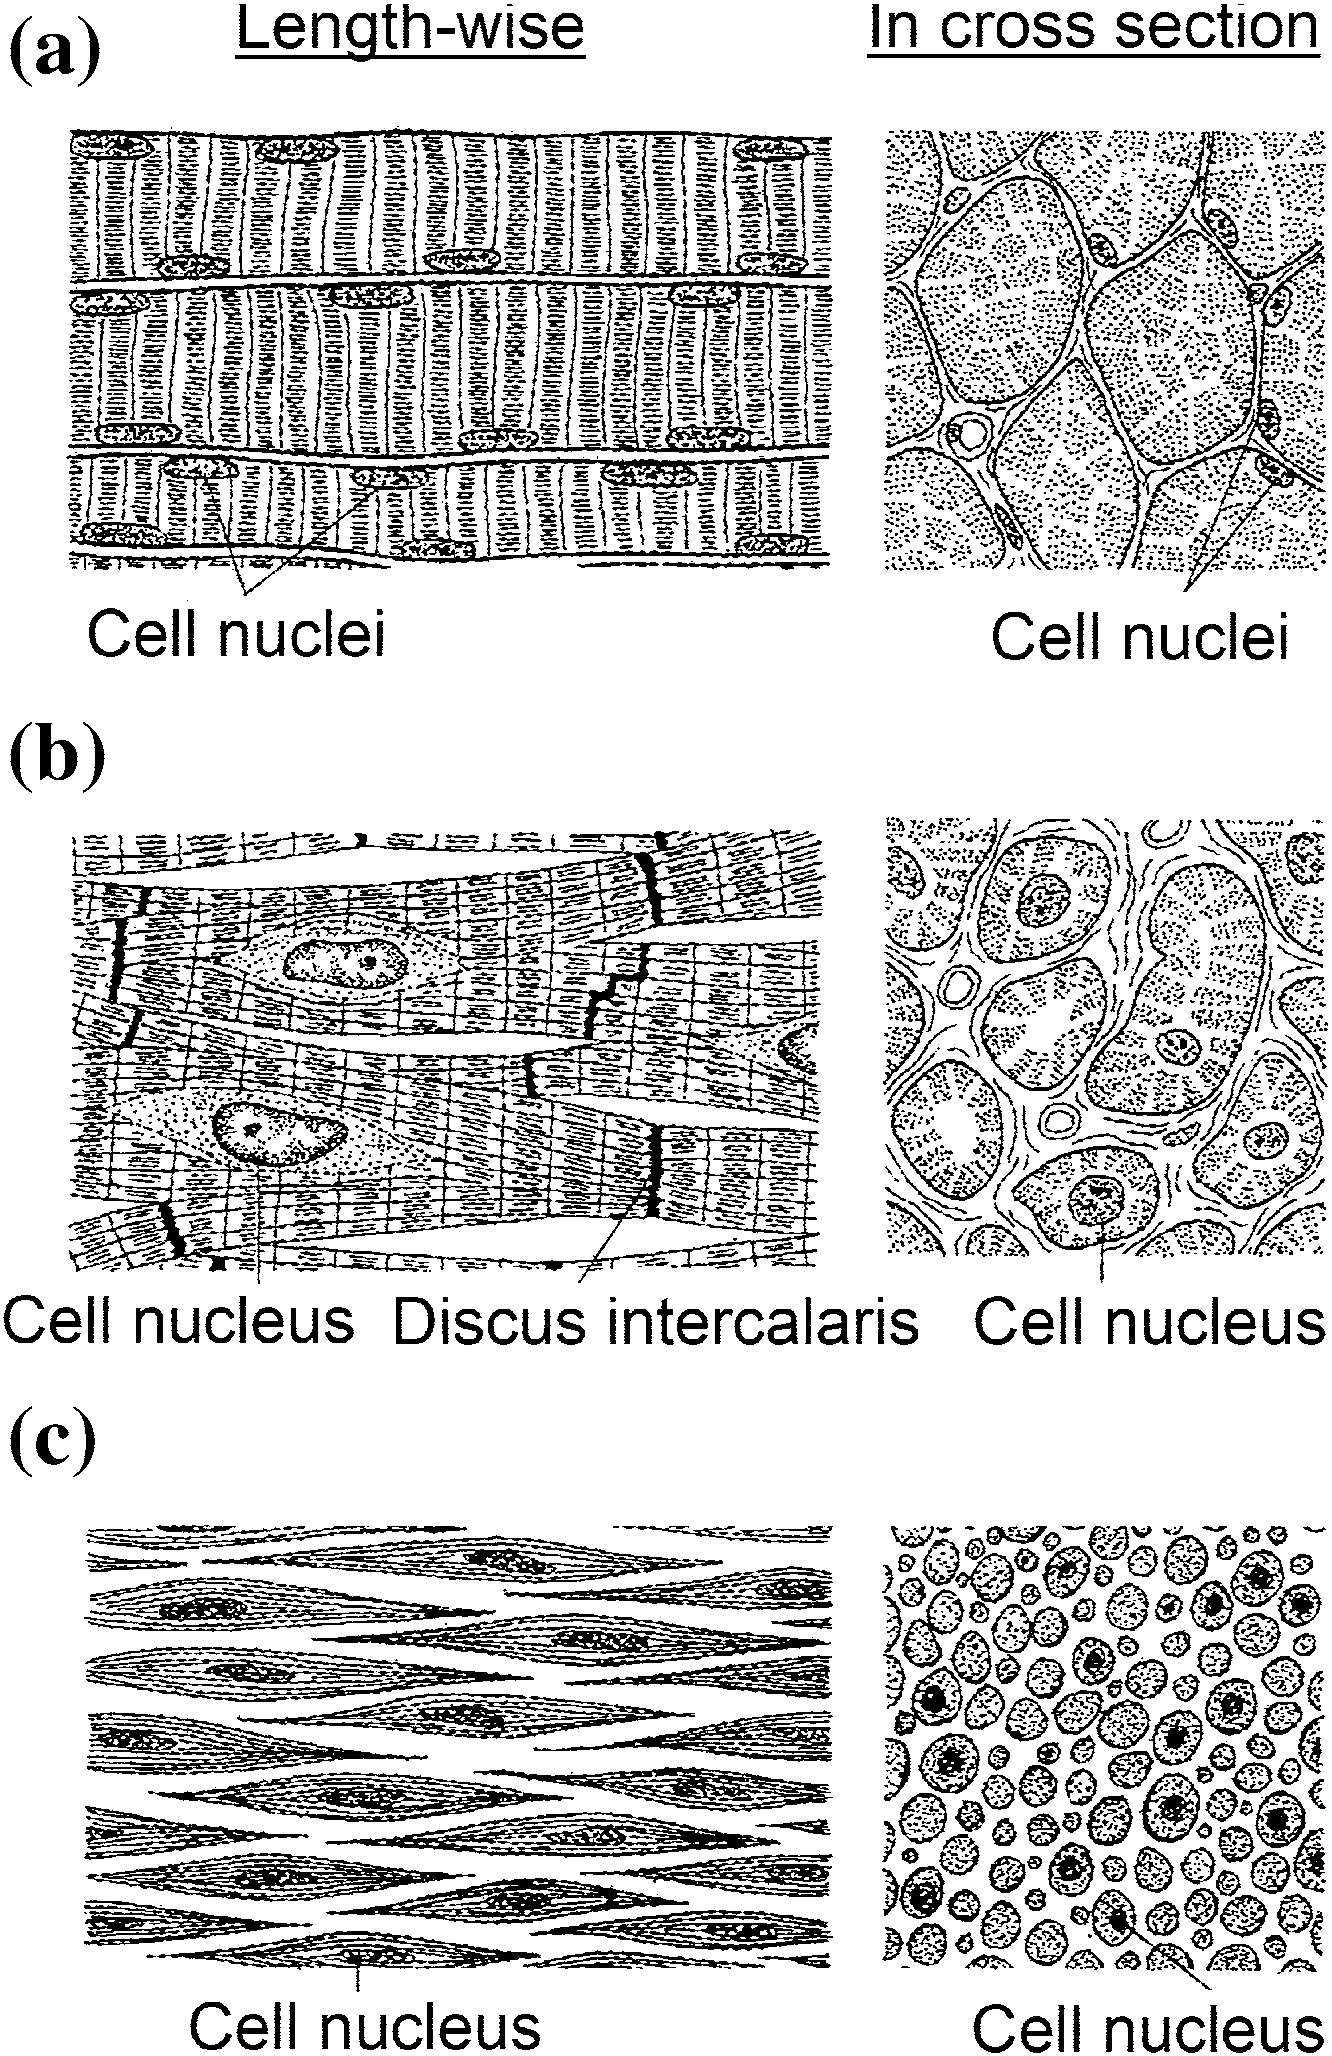
\includegraphics[width=0.45\textwidth]{51.png}
  \caption{Células musculares: \textbf{a} esqueléticas, \textbf{b} cardíacas y \textbf{c} lisas. (De \cite{67})}
  \label{fig:51}
\end{SCfigure}



Aprenderemos cómo funcionan los músculos y desarrollaremos modelos macroscópicos, microscópicos y nanoscópicos de ellos \cite{50, 52, 53, 60, 70, 82}. También volveremos a examinar algunas de las suposiciones que hicimos en capítulos anteriores con respecto a las fuerzas musculares. En el próximo capítulo aprenderemos más sobre cómo se utiliza la energía en los músculos.

\section{Músculos esqueléticos en el cuerpo}

La Figura 1.8 muestra muchos de los principales músculos esqueléticos en el cuerpo.

Los músculos esqueléticos representan aproximadamente el $43\%$ de la masa corporal típica, o alrededor de $30\text{ kg}$ en una persona de $70\text{ kg}$. En reposo, utilizan alrededor del $18\%$ de la tasa de consumo de energía del cuerpo (la cual se denomina tasa metabólica basal o TMB); utilizan mucha más durante las actividades, como el movimiento. Del total de energía ``quemada'' por el músculo esquelético, solo cerca del $25\%$ se utiliza para realizar trabajo, y esta es la eficiencia muscular. El otro $75\%$ restante se libera en forma de calor. (Esta ineficiencia del cuerpo tiene un propósito positivo: es una fuente constante y muy importante de calor corporal).

La fuerza muscular máxima $F_{\text{M}}$ o tensión $T$ que un músculo puede desarrollar es $k_{\text{M}}\text{PCA}$, donde $\text{PCA}$ es el área de sección transversal fisiológica del músculo. El rango de los valores máximos de $k_{\text{M}}$ es de $20\text{--}100\text{ N/cm}^2$ durante condiciones isométricas (longitud constante); los valores mayores corresponden a músculos con la estructura de fibra pinnada que se describe a continuación. (Ver la Fig. 5.46 abajo y el Problema 5.2). En los cuádriceps, las fuerzas alcanzan hasta $\sim 70\text{ N/cm}^2$ al correr y saltar, y $\sim 100\text{ N/cm}^2$ en condiciones isométricas. Discutiremos esto más adelante.

Se sabe que los contramovimientos antes de un movimiento repentino mejoran el rendimiento deportivo \cite{63}. Ponerse en cuclillas rápidamente antes de realizar saltos desde cuclillas conduce a saltos más altos. No se sabe si este estiramiento previo permite más tiempo para que los músculos se activen, optimiza las longitudes y fuerzas del sarcómero (ver más abajo), induce la activación de otros músculos o almacena energía elástica en los tendones, ligamentos o componentes elásticos de los músculos. Este contramovimiento puede ser la razón por la cual las pelotas se pueden lanzar más rápido con un balanceo preparatorio (\textit{windup}) durante el lanzamiento en el béisbol, y esto podría deberse al almacenamiento y posterior liberación de energía elástica.

\begin{table}[htbp]
\centering
\caption{Porcentaje de PCA de los músculos que cruzan la articulación de la cadera}
\label{tab:51}
\begin{tabularx}{0.6\textwidth}{Xc}
\toprule
\textbf{Músculo} & \textbf{\%PCA} \\
\midrule
Iliopsoas & 9 \\
Sartorio & 1 \\
Pectíneo & 1 \\
Recto femoral & 7 \\
Glúteo mayor & 16 \\
Glúteo medio & 12 \\
Glúteo menor & 6 \\
Aductor mayor & 11 \\
Aductor largo & 3 \\
Aductor corto & 3 \\
Tensor de la fascia lata & 1 \\
Bíceps femoral (largo) & 6 \\
Semitendinoso & 3 \\
Semimembranoso & 8 \\
Piriforme & 2 \\
Rotadores laterales & 13 \\
\bottomrule
\end{tabularx}
\begin{flushleft}
    \small Obtenido de \cite{81}, datos de \cite{76}.
\end{flushleft}
\end{table}

A veces se utiliza en los cálculos del movimiento la estimación de que se genera un máximo de $\sim 250\text{--}500\text{ W}$ por $\text{kg}$ de músculo activo para condiciones isotónicas (tensión constante) (y $1,75\times$ esto con estiramiento previo) \cite{13, 25, 78, 79}. Debido a que esto se promedia sobre las áreas, longitudes y velocidades de los músculos que causan el movimiento, por lo general utilizaremos la fuerza muscular por unidad de área en el análisis.

Muchos músculos que cruzan las articulaciones de la cadera, la rodilla y el tobillo son importantes en la locomoción. La importancia relativa de estos músculos de la pierna depende de las ubicaciones de sus puntos de origen e inserción, sus longitudes y sus $\text{PCA}$. Bastantes de estos músculos se representan en las Figs. 3.3, 3.4 y 3.5. (Conjuntos análogos de músculos participan en el control de nuestros brazos y manos, como se ve más adelante en las Figs. 5.22 y 5.23). Las $\text{PCA}$ relativas se presentan en las Tablas 5.1, 5.2 y 5.3. En general, los músculos más largos permiten mayores ángulos de rotación alrededor de las articulaciones. Cuanto mayor sea la $\text{PCA}$ del músculo, mayor será la fuerza muscular. Los músculos con $\text{PCA}$ más pequeñas pueden ser importantes para proporcionar estabilidad.

Como se desprende de las Figs. 1.8 y 3.2 y de las Tablas 5.1, 5.2 y 5.3, muchos de estos músculos de la pierna pasan por más de una articulación. La Figura 5.2 muestra los tres músculos biarticulares (de dos articulaciones) principales en la pierna. Las fuerzas ejercidas por los músculos sobre los huesos en los puntos de origen e inserción son las mismas (Tercera Ley de Newton), pero los torques son diferentes en las articulaciones proximal y distal debido a que los brazos de momento son diferentes. Como se ve en la Fig. 5.2, el gastrocnemio es un flexor de la rodilla y un plantarflexor (extensor) del tobillo, siendo el torque alrededor de esta última articulación mayor debido a su mayor brazo de momento ($5\text{ cm}$ frente a $3,5\text{ cm}$). Durante la bipedestación, el efecto neto de este músculo es hacer que la pierna rote hacia atrás y evitar que la rodilla se colapse.

\begin{figure}[htbp]
  \centering
  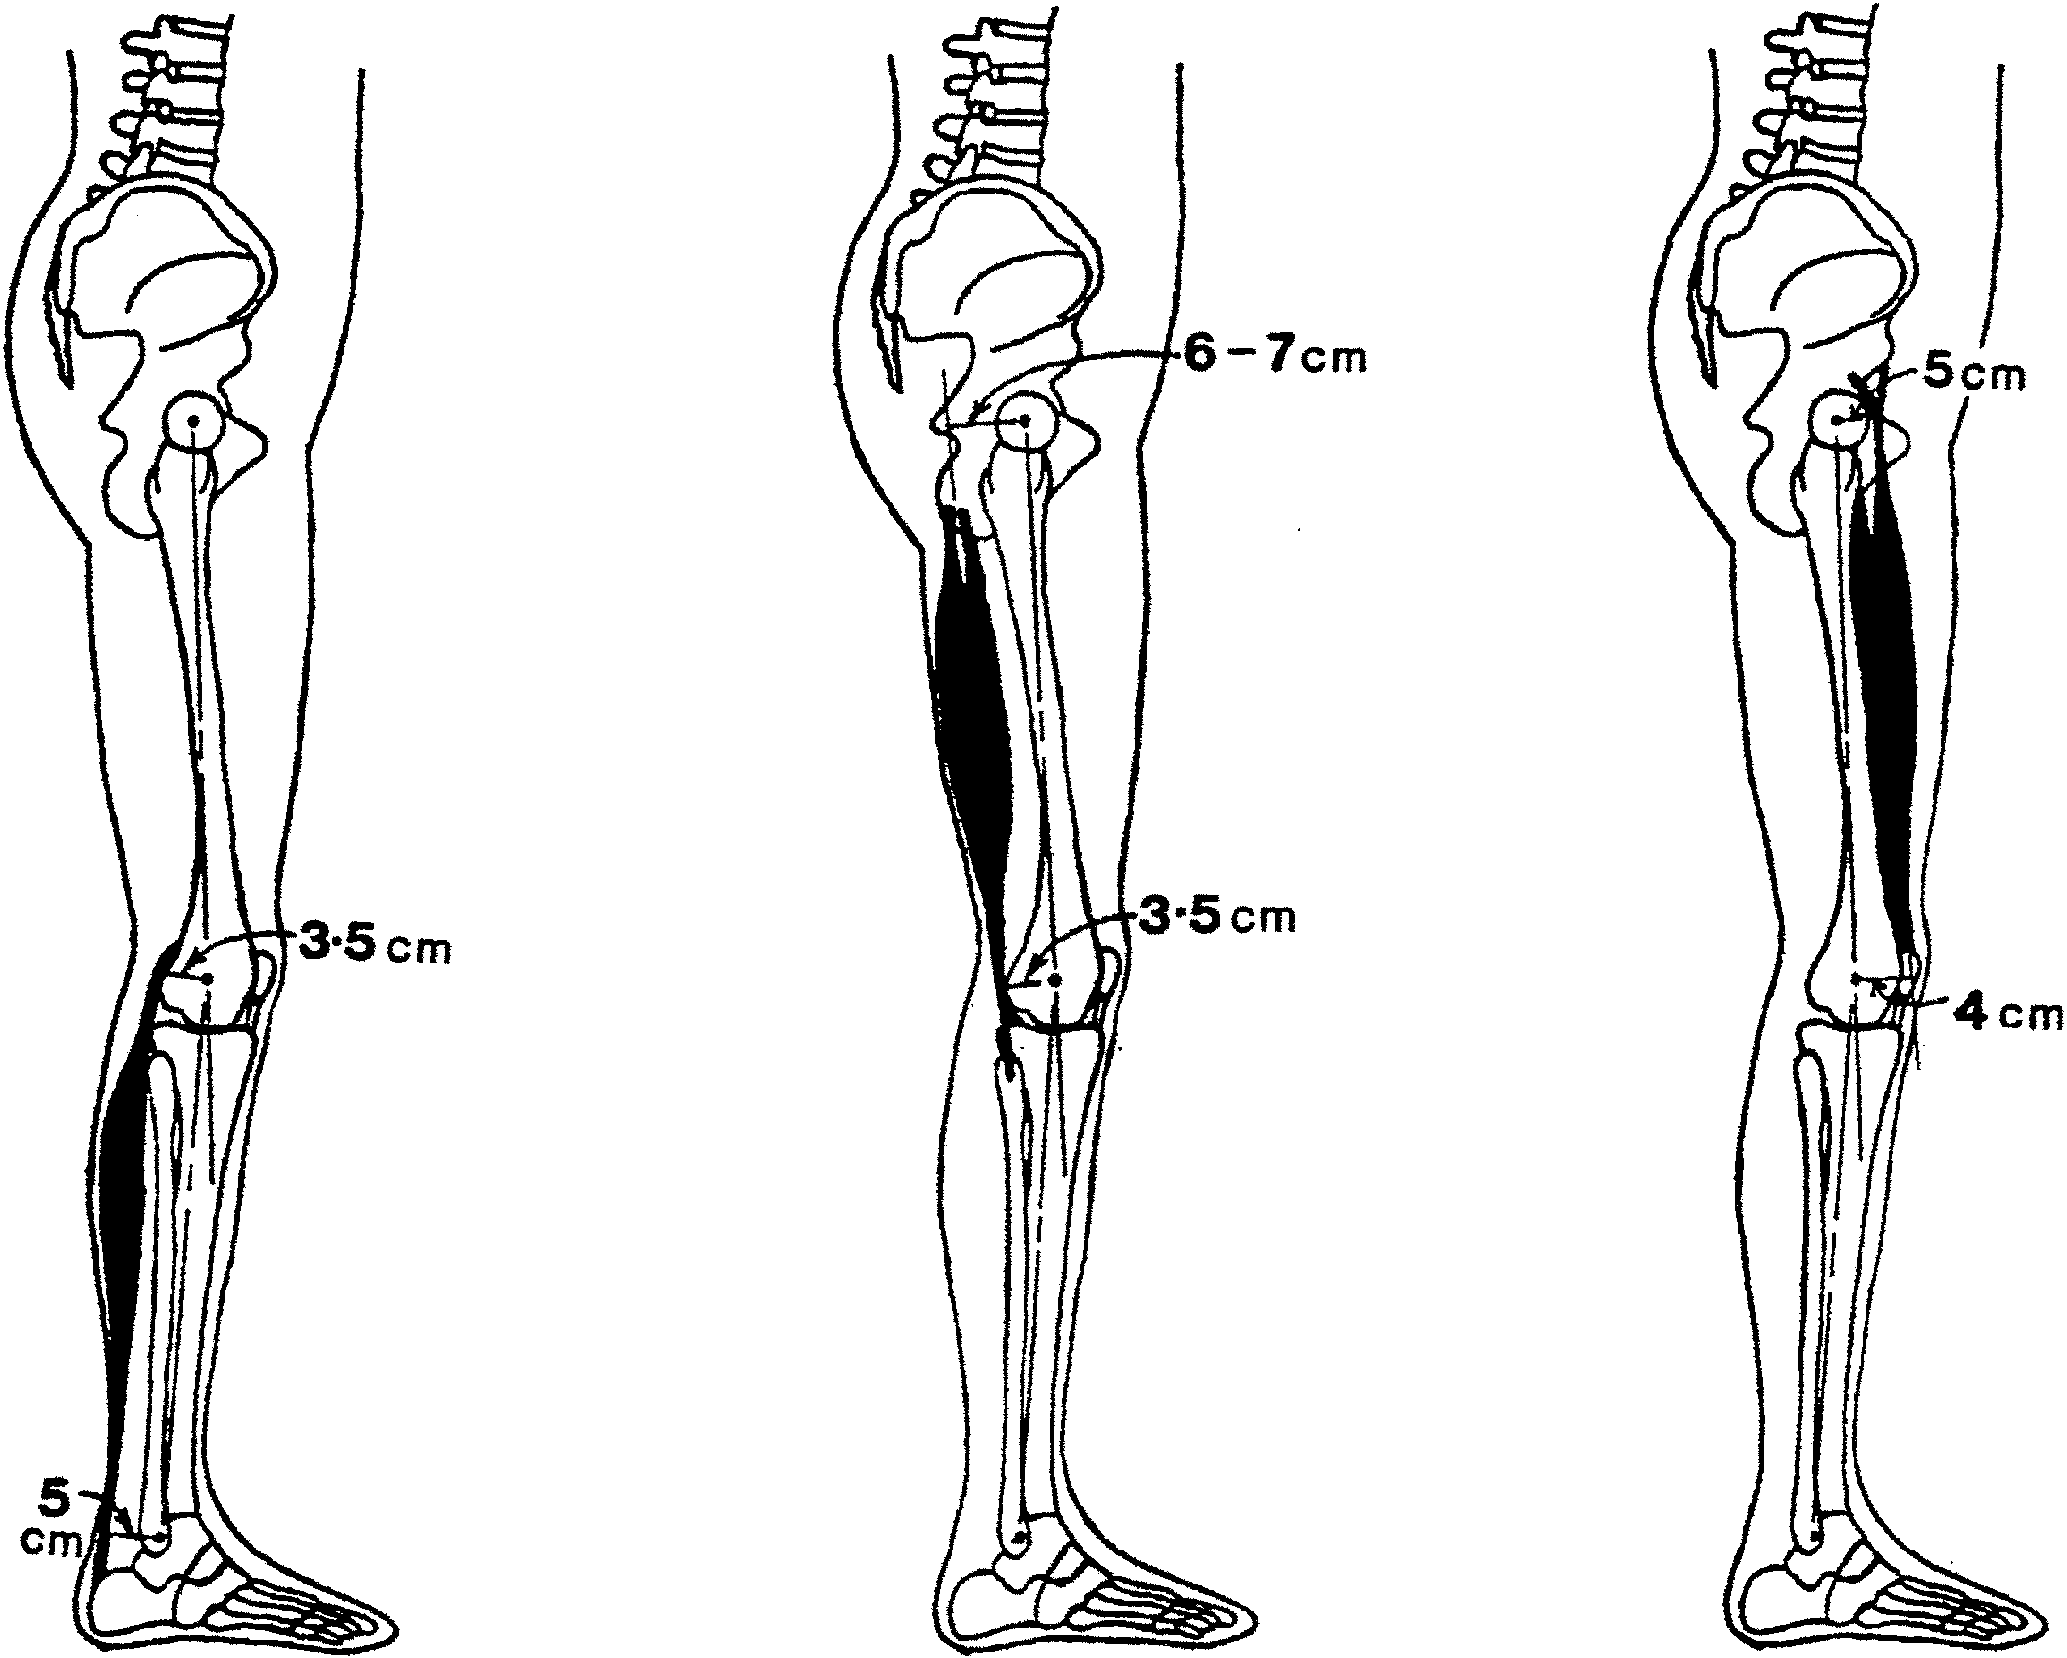
\includegraphics[width=0.7\textwidth]{52.png}
  \caption{Tres músculos biarticulares principales de la pierna: de izquierda a derecha, el gastrocnemio, los isquiotibiales y el recto femoral, junto con las longitudes de sus brazos de momento alrededor de las articulaciones en sus extremos proximal y distal. (De \cite{81}. Reimpreso con autorización de Wiley)}
  \label{fig:52}
\end{figure}



\begin{table}[htbp]
\centering
\caption{Porcentaje de PCA de los músculos que cruzan la articulación de la rodilla}
\label{tab:52}
\begin{tabularx}{0.6\textwidth}{Xc}
\toprule
\textbf{Músculo} & \textbf{\%PCA} \\
\midrule
Gastrocnemio & 19 \\
Bíceps femoral (corto) & 3 \\
Bíceps femoral (largo) & 7 \\
Semitendinoso & 3 \\
Semimembranoso & 10 \\
Vasto lateral & 20 \\
Vasto medial & 15 \\
Vasto intermedio & 13 \\
Recto femoral & 8 \\
Sartorio & 1 \\
Grácil & 1 \\
\bottomrule
\end{tabularx}
\begin{flushleft}
    \small Obtenido de \cite{81}, datos de \cite{76}.
\end{flushleft}
\end{table}

\begin{table}[htbp]
\centering
\caption{Porcentaje de PCA de los músculos que cruzan la articulación del tobillo}
\label{tab:53}
\begin{tabularx}{0.6\textwidth}{Xc}
\toprule
\textbf{Músculo} & \textbf{\%PCA} \\
\midrule
Sóleo & 41 \\
Gastrocnemio & 22 \\
Flexor largo del dedo gordo & 6 \\
Flexor largo de los dedos & 3 \\
Tibial posterior & 10 \\
Peroneo corto & 9 \\
Tibial anterior & 5 \\
Extensor largo de los dedos & 3 \\
Extensor largo del dedo gordo & 1 \\
\bottomrule
\end{tabularx}
\begin{flushleft}
    \small Obtenido de \cite{81}, datos de \cite{76}.
\end{flushleft}
\end{table}

Los isquiotibiales son extensores de la cadera y flexores de la rodilla, teniendo la extensión de la cadera el doble del momento que la flexión de la rodilla. Durante la bipedestación, esto hace que el muslo rote hacia atrás y evita que la rodilla se colapse. El recto femoral del cuádriceps es un flexor de la cadera y extensor de la rodilla, con un brazo de momento ligeramente mayor alrededor de la cadera. Sin embargo, la acción principal del cuádriceps es la extensión de la rodilla debido a que el $84\%$ de la $\text{PCA}$ del cuádriceps proviene de otros músculos, los extensores de la rodilla uniarticulares (y todos estos músculos se activan simultáneamente). El efecto neto de estos tres músculos biarticulares principales es la extensión de las tres articulaciones de la pierna, y ayudan a evitar el colapso debido a la gravedad. Se requiere el movimiento coordinado de estos músculos, como el alargamiento de uno de ellos y el acortamiento de otro, para lograr el rango completo de rotación de estas articulaciones debido al cambio limitado de longitud muscular de cualquiera de ellos \cite{81}.

\subsection{Tipos de actividad muscular}

Los músculos se pueden activar bajo una amplia gama de condiciones. Cuando la longitud del músculo cambia, el ángulo de la articulación correspondiente a este músculo insertado cambia, y hay movimiento en el extremo del hueso que emana de la articulación. Debido a que hay movimiento, se realiza trabajo mecánico. Esto se puede denominar trabajo ``dinámico''. Cuando la longitud del músculo no cambia, es decir, en condiciones isométricas, no hay rotación de la articulación y no se realiza trabajo mecánico. Esto es importante porque el músculo sigue proporcionando tensión para resistir las fuerzas externas, como se requiere para sostener objetos o permanecer de pie. El músculo sigue gastando energía (para dicho trabajo ``estático'') a fin de producir la tensión que resiste la carga.

Se realiza trabajo mecánico con el movimiento de la articulación para contracciones no isométricas. En las contracciones concéntricas, el músculo desarrolla suficiente tensión para vencer la carga y la longitud del músculo se acorta, provocando el movimiento de la articulación. Al subir escaleras, los cuádriceps se contraen y la pierna se endereza como resultado de esta contracción concéntrica. En las contracciones excéntricas, el músculo no desarrolla suficiente tensión para vencer la carga y la longitud del músculo se alarga, a veces ralentizando el movimiento de la articulación (a propósito). Al bajar escaleras, los cuádriceps se activan pero aún se extienden durante este frenado controlado (excéntrico) esencial de la flexión de la rodilla al luchar contra la gravedad. Por lo tanto, los mismos músculos flexores que se contraen concéntricamente durante la flexión pueden contraerse excéntricamente durante la extensión para desacelerar la extensión. Se dice que las contracciones concéntricas realizan trabajo (mecánico) positivo, mientras que las contracciones excéntricas realizan trabajo negativo.

% Control de Calidad: 12 párrafos origen -> 12 párrafos salida. Mapeo 1:1 verificado. Sin omisiones.

Durante la contracción isocinética, la velocidad de acortamiento o alargamiento del músculo y, por consiguiente, también la velocidad angular de la articulación son constantes. Durante la contracción isoinercial, la carga resistiva sobre el músculo (debido a la fuerza de gravedad, fuerzas aplicadas, etc.) es constante. Durante la contracción isotónica, la tensión es constante. (Esta es una condición idealizada debido a que la tensión muscular en realidad cambia con la longitud).

En la flexión del codo, los músculos bíceps braquial y braquial se contraen y son los agonistas o motores primarios de la acción. El braquiorradial es un músculo sinergista en el movimiento; tales músculos sinergistas asisten al movimiento y a veces añaden un ajuste fino. Los tríceps braquiales son los antagonistas de esta acción y se oponen a los motores primarios.

Durante la marcha y la carrera, los cuádriceps actúan excéntricamente durante la fase de apoyo inicial para evitar el colapso del ángulo de la rodilla, y luego concéntricamente para extender la rodilla a medida que la pierna rota sobre el pie en la fase de apoyo medio (y esto ocurre en mayor medida al caminar). Los plantarflexores del tobillo se activan excéntricamente durante el apoyo para ayudar a que la rotación de la pierna sobre el pie avance de manera controlada, y luego concéntricamente para asistir en el despegue.

\section{La estructura de los músculos}

Los músculos tienen una estructura de fibras con niveles sucesivos de subestructuras similares a fibras llamadas fascículos (\textit{fasciculi}). (Uno solo es un fascículo (\textit{fasciculus})). A nivel macroscópico, estas fibras se organizan de una de varias maneras. Esto se ilustra en la Fig. 5.3. Parece que las fuerzas generadas por las fibras musculares individuales y los músculos se pueden sumar de manera independiente \cite{65, 66}.

\begin{figure}[htbp]
  \centering
  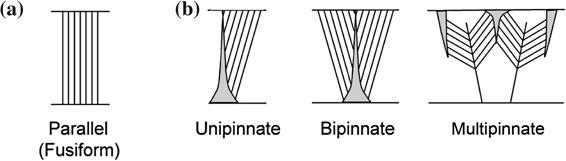
\includegraphics[width=0.8\textwidth]{53.png}
  \caption{Tipos de disposiciones de fibras en los músculos esqueléticos, con fibras \textbf{a} paralelas y \textbf{b} pinnadas. (Basado en \cite{53})}
  \label{fig:53}
\end{figure}



En los músculos fusiformes, las fibras musculares son paralelas y se estrechan y mezclan en tendones que se unen al esqueleto. En los músculos paralelos, las fibras también son paralelas. Tienden a ser largas, como el sartorio (el músculo más largo del cuerpo, que se extiende desde la cadera hasta la tibia (Figs. 1.8 y 5.4)). (Las fibras también son paralelas en el recto del abdomen (los ``abdominales'')). Por lo general, no diferenciaremos entre músculos fusiformes y paralelos debido a su disposición similar de fibras musculares. Estos músculos consisten en muchos componentes de sarcómero en serie (ver más abajo), y como tales pueden acortarse mucho más para producir una gran cantidad de movimiento de los huesos para el movimiento alrededor de las articulaciones, y pueden hacerlo rápidamente. En los músculos unipinnados, las fibras musculares paralelas se unen a los tendones en ángulo, como ocurre con el flexor largo del pulgar (\textit{flexor pollicis longus}, poe-lee'-cis) en la parte inferior de la mano/pulgar y el extensor largo de los dedos (\textit{extensor digitorum longus}, di-gi-tor'-ee-um) en la parte inferior de la pierna/pie. En los músculos bipinnados, tales fibras musculares paralelas se unen a un tendón en dos direcciones diferentes, como ocurre con el recto femoral (\textit{rectus femoris}, fe-more'-is) en el muslo. Estas estructuras pinnadas (o penadas o de pinnación) se asemejan a la estructura de las plumas y de algunas hojas en las ramas. Las fibras se unen al tendón central en varios ángulos en los músculos deltoides multipinnados (hombro). Muchas fibras musculares cortas se pueden unir a tendones tan cortos en los músculos pinnados, lo que conduce a fuerzas mayores que en los músculos paralelos y a un mayor movimiento, pero con un uso menos eficiente de las fuerzas musculares (ver más abajo y el Problema 5.17). El orbicular de los ojos (\textit{orbicularis oculi}, or-bee-queue-lar'-is ok'-you-lie) alrededor del ojo son músculos circulares, en los cuales las fibras musculares están dispuestas en círculo alrededor del objeto. El pectoral mayor (\textit{pectoralis major}, pec-tor-al'-is) en la parte superior del pecho (los ``pectorales'') es un músculo convergente; tales músculos son anchos en su origen y se estrechan en la inserción, lo que conduce a grandes fuerzas cerca del punto de inserción. Ejemplos de cada uno de estos tipos de músculos en el cuerpo se muestran en la Fig. 5.4.

\begin{figure}[htbp]
  \centering
  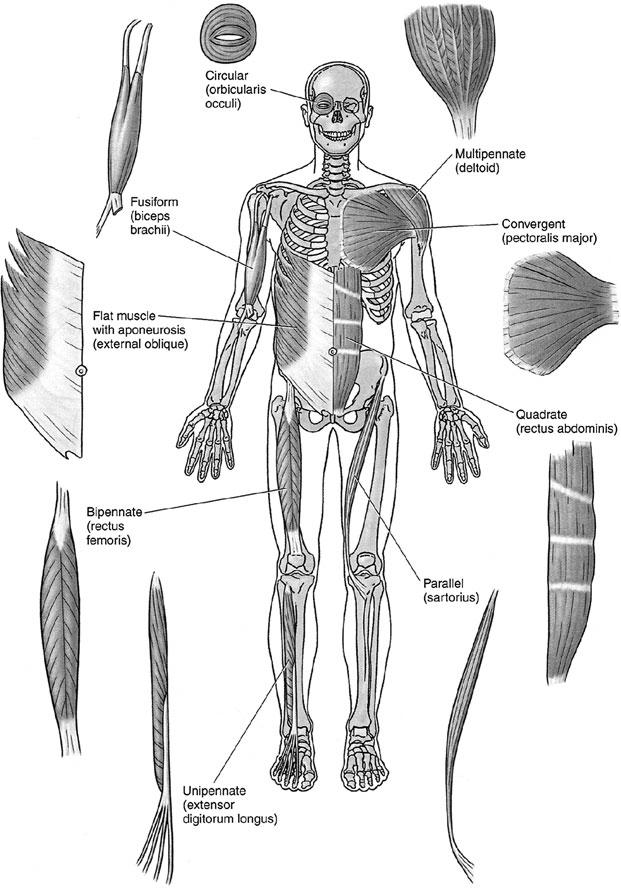
\includegraphics[width=0.45\textwidth]{54.png}
  \caption{Ejemplos de disposiciones de fibras musculares en el cuerpo. (De \cite{58}. Utilizado con autorización)}
  \label{fig:54}
\end{figure}



La manera en que se suman las fuerzas de las fibras musculares para dar la fuerza total sobre el tendón de unión difiere para estas diferentes estructuras musculares. En los músculos paralelos y fusiformes, toda la fuerza de las fibras se transmite al tendón. En los músculos pinnados, las fibras están unidas al tendón en un ángulo $\theta$, y solo $F \cos\theta$ de la fuerza $F$ de cada fibra se transmite efectivamente. Aunque esta es una desventaja notable del diseño pinnado, tiene otras ventajas relativas. Debido a que la geometría permite que las fibras se unan a lo largo de una parte de la longitud del tendón (Fig. 5.5), se pueden unir muchas más fibras al tendón. Además, esta geometría permite que el tendón central se mueva una distancia mayor que en el esquema fusiforme, por lo que los huesos unidos al tendón pueden moverse más. Esto supera el cambio limitado de longitud en los músculos que puede limitar el rango de movimiento angular de los huesos alrededor de las articulaciones. Estos temas y otros relacionados se abordan en el Problema 5.17. La masa, la longitud de la fibra, la $\text{PCA}$ y el ángulo de pinnación $\theta$ para varios músculos se presentan en la Tabla 5.4.

\begin{SCfigure}[0.8][htbp]
  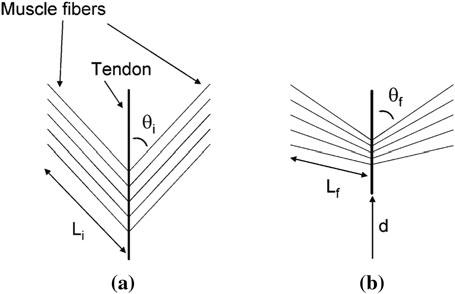
\includegraphics[width=0.55\textwidth]{55.png}
  \caption{Fibras musculares en músculos pinnados: \textbf{a} antes y \textbf{b} después de la contracción de las fibras con el consiguiente movimiento del tendón.}
  \label{fig:55}
\end{SCfigure}



\begin{table}[htbp]
\centering
\caption{Propiedades de algunos músculos}
\label{tab:54}
\begin{tabularx}{\textwidth}{Xcccc}
\toprule
\textbf{Músculo} & \textbf{Masa (g)} & \textbf{Longitud de fibra (cm)} & \textbf{PCA ($\text{cm}^2$)} & \textbf{Ángulo de pinnación ($^\circ$)} \\
\midrule
Sartorio & 75 & 38 & 1,9 & 0 \\
Bíceps femoral (largo) & 150 & 9 & 15,8 & 0 \\
Semitendinoso & 75 & 16 & 4,4 & 0 \\
Sóleo & 215 & 3,0 & 58 & 30 \\
Gastrocnemio & 158 & 4,8 & 30 & 15 \\
Tibial posterior & 55 & 2,4 & 21 & 15 \\
Tibial anterior & 70 & 7,3 & 9,1 & 5 \\
Recto femoral & 90 & 6,8 & 12,5 & 5 \\
Vasto lateral & 210 & 6,7 & 30 & 5 \\
Vasto medial & 200 & 7,2 & 26 & 5 \\
Vasto intermedio & 180 & 6,8 & 25 & 5 \\
\bottomrule
\end{tabularx}
\begin{flushleft}
    \small Obtenido de \cite{81}, datos de \cite{76}.
\end{flushleft}
\end{table}

Los componentes microscópicos de las fibras se ilustran en las Figs. 5.6 y 5.7, donde se observa que el vientre muscular de un músculo fusiforme está compuesto por muchos fascículos paralelos. Cada fascículo está compuesto por muchas fibras musculares (o células musculares) paralelas. Cada fibra muscular está compuesta por muchas miofibrillas paralelas. Cada miofibrilla está compuesta por miofilamentos organizados en unidades de $\sim 2\text{--}3\ \mu\text{m}$ de largo llamadas sarcómeros (\textit{sarcomeres}, sar'-koe-meres). Existen miofilamentos gruesos con una disposición en serie de muchas moléculas de miosina (\textit{myosin}, my'-oh-sin) y miofilamentos delgados con glóbulos de moléculas de F-actina (o actina) que forman filamentos helicoidales, los cuales están rodeados por otras dos proteínas: la tropomiosina (que forma filamentos que se enrollan alrededor de los filamentos de actina) y la troponina T (que se une a intervalos regulares a los filamentos de actina y tropomiosina). La interacción entre las proteínas miosina y actina en miofilamentos adyacentes es la interacción fundamental, inducida químicamente y productora de fuerza en el músculo, la cual involucga la hidrólisis de ATP y el cambio en la conformación de la miosina.

\begin{figure}[htbp]
  \centering
  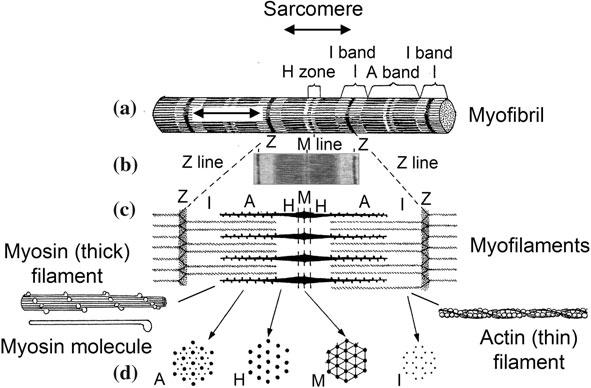
\includegraphics[width=0.7\textwidth]{56.png}
  \caption{Organización de los músculos esqueléticos, hasta el nivel de las miofibrillas. Ver la Fig. 5.7 para la estructura de la miofibrilla. (De \cite{68})}
  \label{fig:56}
\end{figure}

\begin{figure}[htbp]
  \centering
  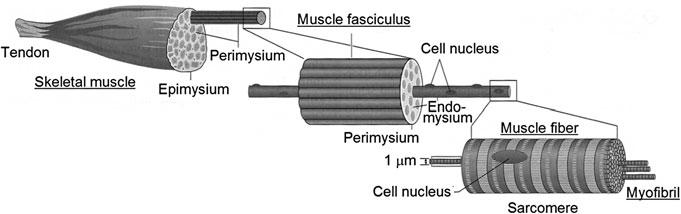
\includegraphics[width=0.8\textwidth]{57.png}
  \caption{\textbf{a} Estructura y subestructura de la miofibrilla mostrada en la Fig. 5.6, con la estructura en bandas de los sarcómeros (cuya periodicidad se denota con las flechas). \textbf{b} La micrografía electrónica de barrido de un músculo esquelético muestra la estructura de bandas y líneas en los sarcómeros. Esto se asocia con los filamentos gruesos y delgados en \textbf{c} desde la perspectiva longitudinal de (a) y (b); la sección transversal se observa en \textbf{d}. (De \cite{67})}
  \label{fig:57}
\end{figure}



En la extremidad grande de un adulto, las fibras musculares tienen un diámetro de $\sim 50\ \mu\text{m}$. Este diámetro se puede duplicar con el entrenamiento con pesas. Dependiendo del tipo de músculo, existen de $\sim 10^4\text{--}10^7$ fibras musculares por músculo (Tabla 5.5). Hay entre $\sim 1 \times 10^4\text{--}1,7 \times 10^5$ sarcómeros por fibra muscular, según el tipo de músculo (Tabla 5.6).

La micrografía electrónica en la Fig. 5.7 muestra la estructura de miofilamentos en bandas que también se bosqueja en la figura. La banda A es una región ancha y oscura, anisotrópica, mientras que la banda I es una región ancha y clara, isotrópica. Existe una zona o banda H más clara en medio de la banda oscura A, y una línea M más oscura en medio de la zona H. Las líneas oscuras Z atraviesan las bandas claras I.

Cada sarcómero está delimitado entre las líneas Z adyacentes. La banda A oscura en el centro de cada sarcómero consiste en miofilamentos gruesos (de miosina) (o filamentos gruesos), los cuales están conectados entre sí en la línea central M dentro de la zona H. Están superpuestos en cierta medida por los miofilamentos delgados (de actina) (o filamentos delgados). Hay filamentos gruesos pero no filamentos delgados en la zona H central. Las regiones claras de la banda I junto a las líneas Z son los miofilamentos delgados en las regiones donde no se superponen con los miofilamentos gruesos; están unidos entre sí en la línea Z. Esto se muestra de forma esquemática en la Fig. 5.7.

% Control de Calidad: 10 párrafos origen -> 10 párrafos salida. Mapeo 1:1 verificado. Sin omisiones.

\begin{table}[htbp]
\centering
\caption{Número de fibras musculares en los músculos humanos}
\label{tab:55}
\begin{tabularx}{0.6\textwidth}{Xc}
\toprule
\textbf{Músculo} & \textbf{Número de fibras musculares} \\
\midrule
Primer lumbrical & 10.250 \\
Recto externo & 27.000 \\
Platisma & 27.000 \\
Primer interóseo dorsal & 40.500 \\
Sartorio & 128.150 \\
Braquiorradial & 129.200 \\
Tibial anterior & 271.350 \\
Gastrocnemio medial & 1.033.000 \\
\bottomrule
\end{tabularx}
\begin{flushleft}
    \small Utilizando datos de \cite{52}
\end{flushleft}
\end{table}

\begin{table}[htbp]
\centering
\caption{Número de sarcómeros en los músculos humanos}
\label{tab:56}
\begin{tabularx}{\textwidth}{Xccc}
\toprule
\textbf{Músculo} & \multicolumn{3}{c}{\textbf{Número de sarcómeros por fibra ($\times 10^4$)}} \\
\cmidrule(lr){2-4}
 & \textbf{Persona I} & \textbf{Persona II} & \textbf{Persona III} \\
\midrule
Tibial posterior & 1,1 & 1,5 & 0,8 \\
Sóleo & 1,4 & -- & -- \\
Gastrocnemio medial & 1,6 & 1,5 & 1,5 \\
Semitendinoso & 5,8 & 6,6 & -- \\
Grácil & 8,1 & 9,3 & 8,4 \\
Sartorio & 15,3 & 17,4 & 13,5 \\
\bottomrule
\end{tabularx}
\begin{flushleft}
    \small Utilizando datos de \cite{52}
\end{flushleft}
\end{table}

\section{Activación de los músculos: perspectiva macroscópica}

Los estímulos eléctricos producen sacudidas musculares que aumentan temporalmente la fuerza ejercida por los músculos. Estas sacudidas se retrasan unos $15\text{ ms}$ después del estímulo eléctrico. Alcanzan su valor máximo $\sim 40\text{ ms}$ más tarde, y luego decaen a cero $\sim 50\text{ ms}$ después (Fig. 5.8a, Tabla 5.7). La forma de una sacudida se puede modelar como
\begin{equation}
F(t) = F_0 \frac{t}{T} \exp(-t/T),
\label{eq:5.1}
\end{equation}
con un tiempo de sacudida $T$.

Al aumentar la frecuencia de estos estímulos y, por consiguiente, de las sacudidas, se produce un incremento en la fuerza ejercida por el músculo (Fig. 5.8b, c). A una frecuencia suficientemente alta, las sacudidas se superponen para producir un nivel de fuerza casi constante llamado tétanos incompleto (o no fusionado), y a una frecuencia aún mayor producen una fuerza constante en el tiempo llamada tétanos completo (o fusionado) (Fig. 5.9). Se requieren aproximadamente $50\text{--}60$ descargas eléctricas por segundo para tetanizar completamente los músculos de mamíferos a temperatura ambiente. Esto varía desde aproximadamente $\sim 30/\text{s}$ para el músculo sóleo hasta $\sim 300/\text{s}$ para los músculos oculares. (Ver también la Fig. 5.11 más abajo).

\begin{SCfigure}[0.8][htbp]
  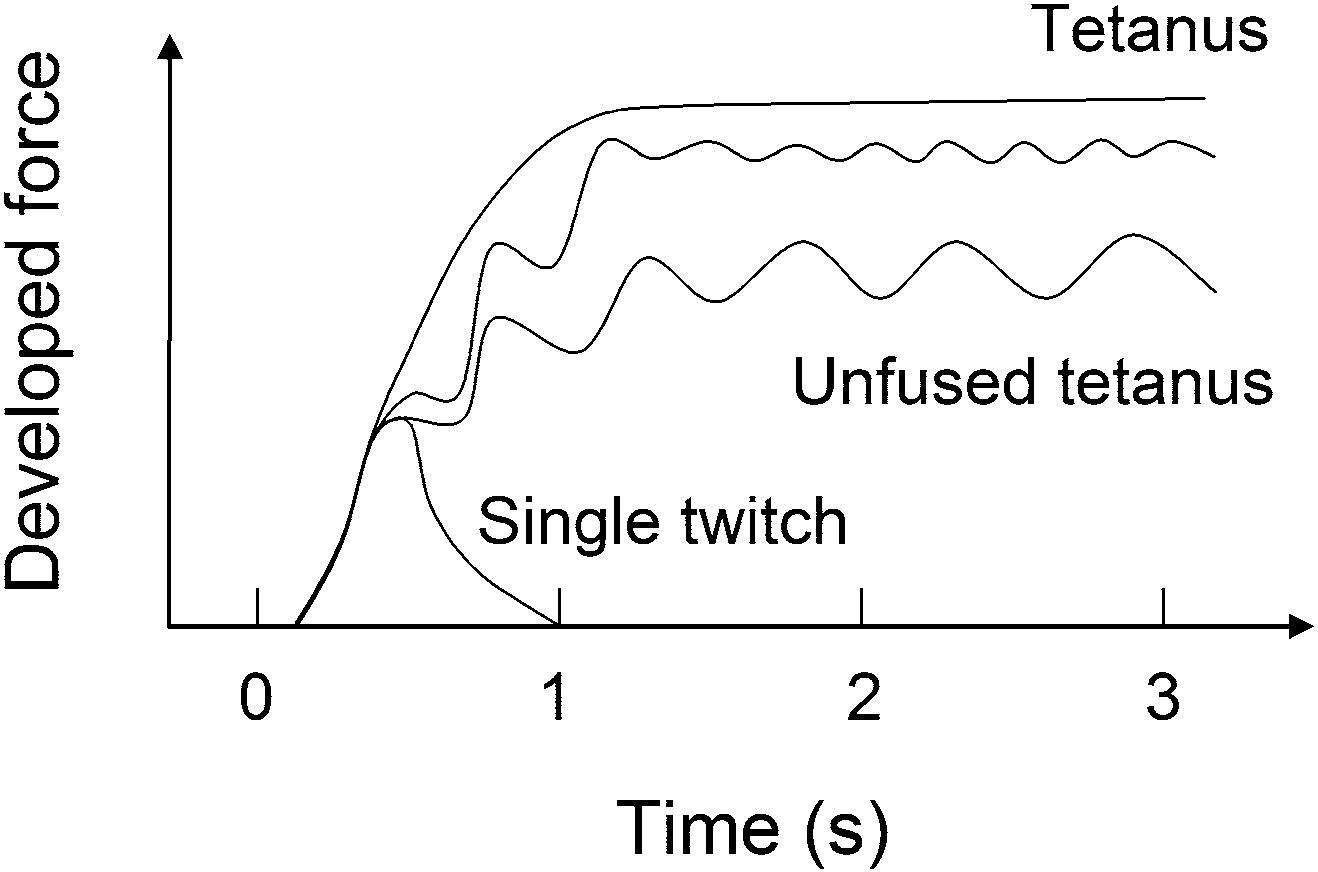
\includegraphics[width=0.55\textwidth]{58.png}
  \caption{Dos sacudidas estimuladas en S1 y S2, con diversos retrasos. (Basado en \cite{53})}
  \label{fig:58}
\end{SCfigure}

\begin{SCfigure}[0.9][htbp]
  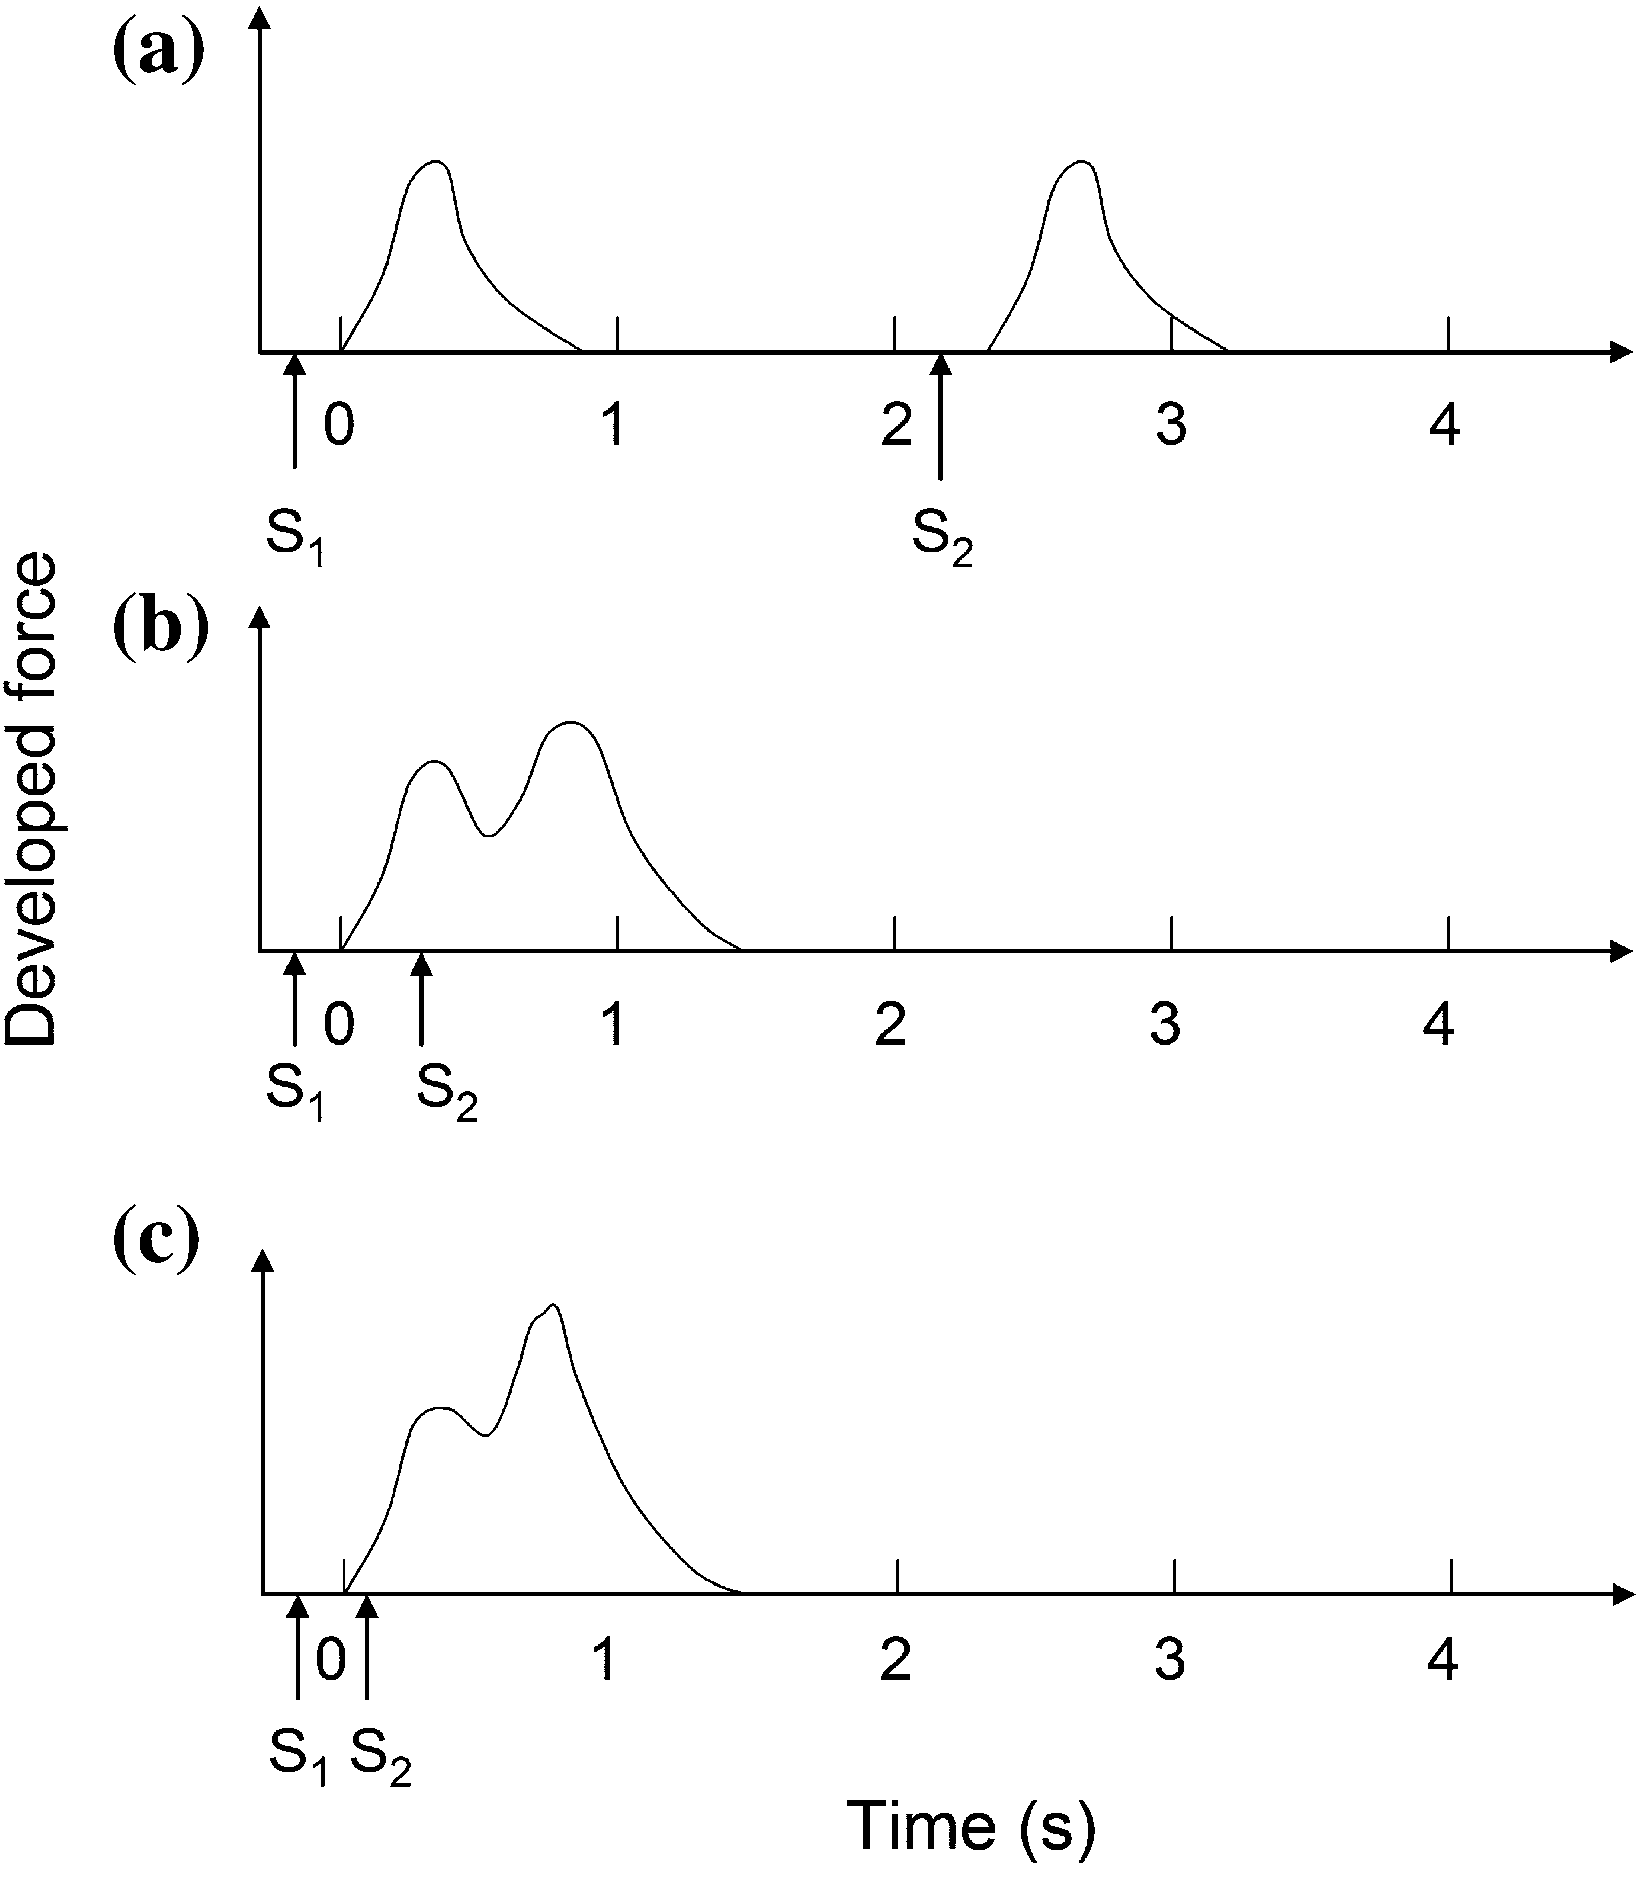
\includegraphics[width=0.5\textwidth]{59.png}
  \caption{Una sacudida, seguida de una serie de sacudidas que conducen a un tétanos incompleto y, a una frecuencia aún mayor, conducen al tétanos completo. (Basado en \cite{53})}
  \label{fig:59}
\end{SCfigure}



\begin{table}[htbp]
\centering
\caption{Tiempo de sacudida $T$, en ms}
\label{tab:57}
\begin{tabularx}{0.7\textwidth}{Xcc}
\toprule
\textbf{Músculo} & \textbf{Tiempo medio típico} & \textbf{Rango de tiempos} \\
\midrule
Tríceps braquial & 44,5 & 16--68 \\
Bíceps braquial & 52,0 & 16--85 \\
Tibial anterior & 58,0 & 38--80 \\
Sóleo & 74,0 & 52--100 \\
Gastrocnemio medial & 79,0 & 40--110 \\
\bottomrule
\end{tabularx}
\begin{flushleft}
    \small Utilizando datos de \cite{81}
\end{flushleft}
\end{table}

Existen tres tipos diferentes de fibras musculares, las cuales difieren en la rapidez con la que se contraen y en su resistencia a la fatiga. Aparecen en diferentes tipos de músculos en proporciones variables (Fig. 5.10). Para un tipo de músculo dado, sus concentraciones relativas pueden ser diferentes en distintas personas. Las fibras rojas de contracción lenta (ST, del inglés \textit{slow-twitch}) (Tipo I) tienen un tiempo de contracción prolongado ($\sim 110\text{ ms}$) y son muy resistentes a la fatiga debido a que son aeróbicas, es decir, utilizan oxígeno para producir ATP. Estas fibras son rojas porque disponen de sangre para suministrar oxígeno. Las fibras de contracción rápida (FT, del inglés \textit{fast-twitch}) por lo general pueden generar más fuerza que las fibras ST y alcanzan una tensión máxima en menos tiempo ($\sim 50\text{ ms}$). Las fibras intermedias rojas FT (Tipo IIA) tienen un tiempo de contracción relativamente corto, una tasa de fatiga intermedia y generación aeróbica de ATP. Las fibras blancas FT (Tipo IIB) tienen un tiempo de contracción corto y se fatigan rápidamente debido a que utilizan procesos anaeróbicos (es decir, sin oxígeno) para producir ATP. Una de las razones de la respuesta más rápida del músculo de contracción rápida es la neurona de mayor tamaño que lo excita.

\begin{figure}[htbp]
  \centering
  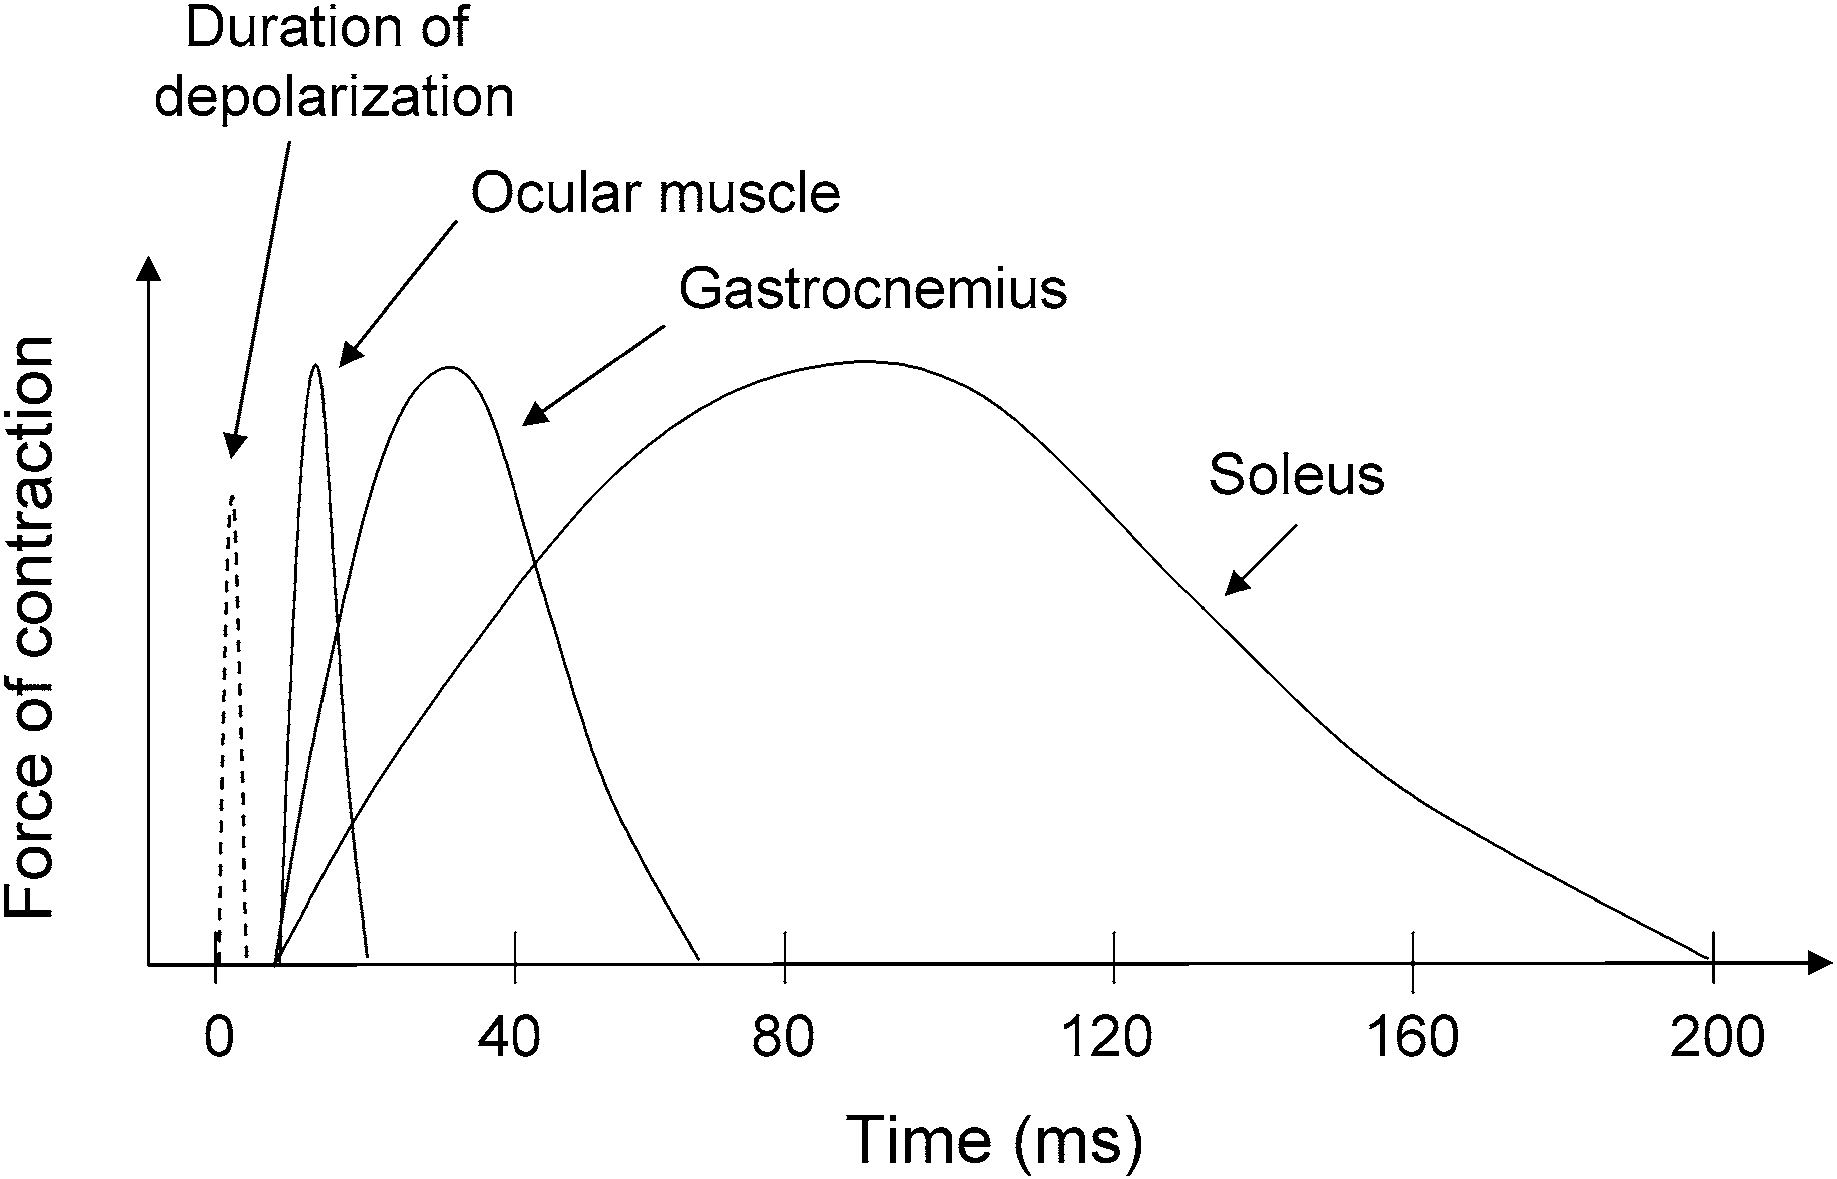
\includegraphics[width=0.7\textwidth]{510.png}
  \caption{Fotomicrografía de células musculares teñidas de un músculo vasto lateral humano, que muestra células ST Tipo I (oscuras) y FT Tipo II (ligeramente teñidas), con líneas finas añadidas que muestran los límites. (De \cite{20}. Utilizado con autorización)}
  \label{fig:510}
\end{figure}



El músculo ``promedio'' tiene aproximadamente el $50\%$ de fibras ST y el $25\%$ de fibras FT rojas y blancas. El tiempo de contracción de un músculo depende de la proporción de fibras FT y ST. La Figura 5.11 muestra la respuesta de sacudida para tres tipos de músculos. Los músculos oculares del ojo tienen en su mayoría músculos FT y un tiempo de respuesta de $\sim 1/40\text{ s}$. El músculo gastrocnemio (\textit{gastrocnemius}, gas-trok-nee'-mee-us) tiene muchos músculos FT y un tiempo de respuesta de $\sim 1/15\text{ s}$. El músculo sóleo (\textit{soleus}, soh'-lee-us) tiene muchos músculos ST y un tiempo de respuesta de $\sim 1/5\text{ s}$.

\begin{figure}[htbp]
  \centering
  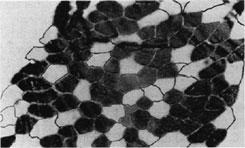
\includegraphics[width=0.8\textwidth]{511.png}
  \caption{Duración de las respuestas isométricas para diferentes músculos con diferentes fibras musculares FT y ST. (Basado en \cite{26})}
  \label{fig:511}
\end{figure}



Todo esto tiene sentido en términos de las necesidades del cuerpo. Los músculos oculares deben ser rápidos para el reflejo ocular rápido que requerimos. Los músculos gastrocnemio y sóleo en la parte superior de la pantorrilla están conectados al tendón de Aquiles (calcáneo) en el pie, el cual está conectado al hueso calcáneo en el talón. El músculo sóleo es un músculo ancho de la pantorrilla que es profundo en relación con las cabezas medial y lateral del músculo gastrocnemio (ver Figs. 1.8b y 3.5). El músculo sóleo se utiliza más para la bipedestación y la estabilidad, para las cuales la resistencia y la tolerancia a la fatiga son importantes y una respuesta rápida no es muy relevante. El músculo gastrocnemio se utiliza principalmente para saltar y correr, actividades para las cuales es necesaria una respuesta rápida, incluso a expensas de la resistencia. La fracción relativa de músculos ST y FT en la rodilla para atletas entrenados se representa en la Fig. 5.12 y en la Tabla 5.8. Claramente, los atletas en deportes que requieren resistencia (como los corredores de maratón) tienen una mayor fracción de fibras musculares ST en los músculos utilizados para correr, mientras que aquellos en deportes que requieren velocidad y fuerza (como los velocistas y los levantadores de pesas) tienen una mayor fracción de músculos FT en los músculos que se utilizan intensamente en estas actividades. Existe una correlación similar para las áreas de sección transversal de estas diferentes fibras musculares.

\begin{figure}[htbp]
  \centering
  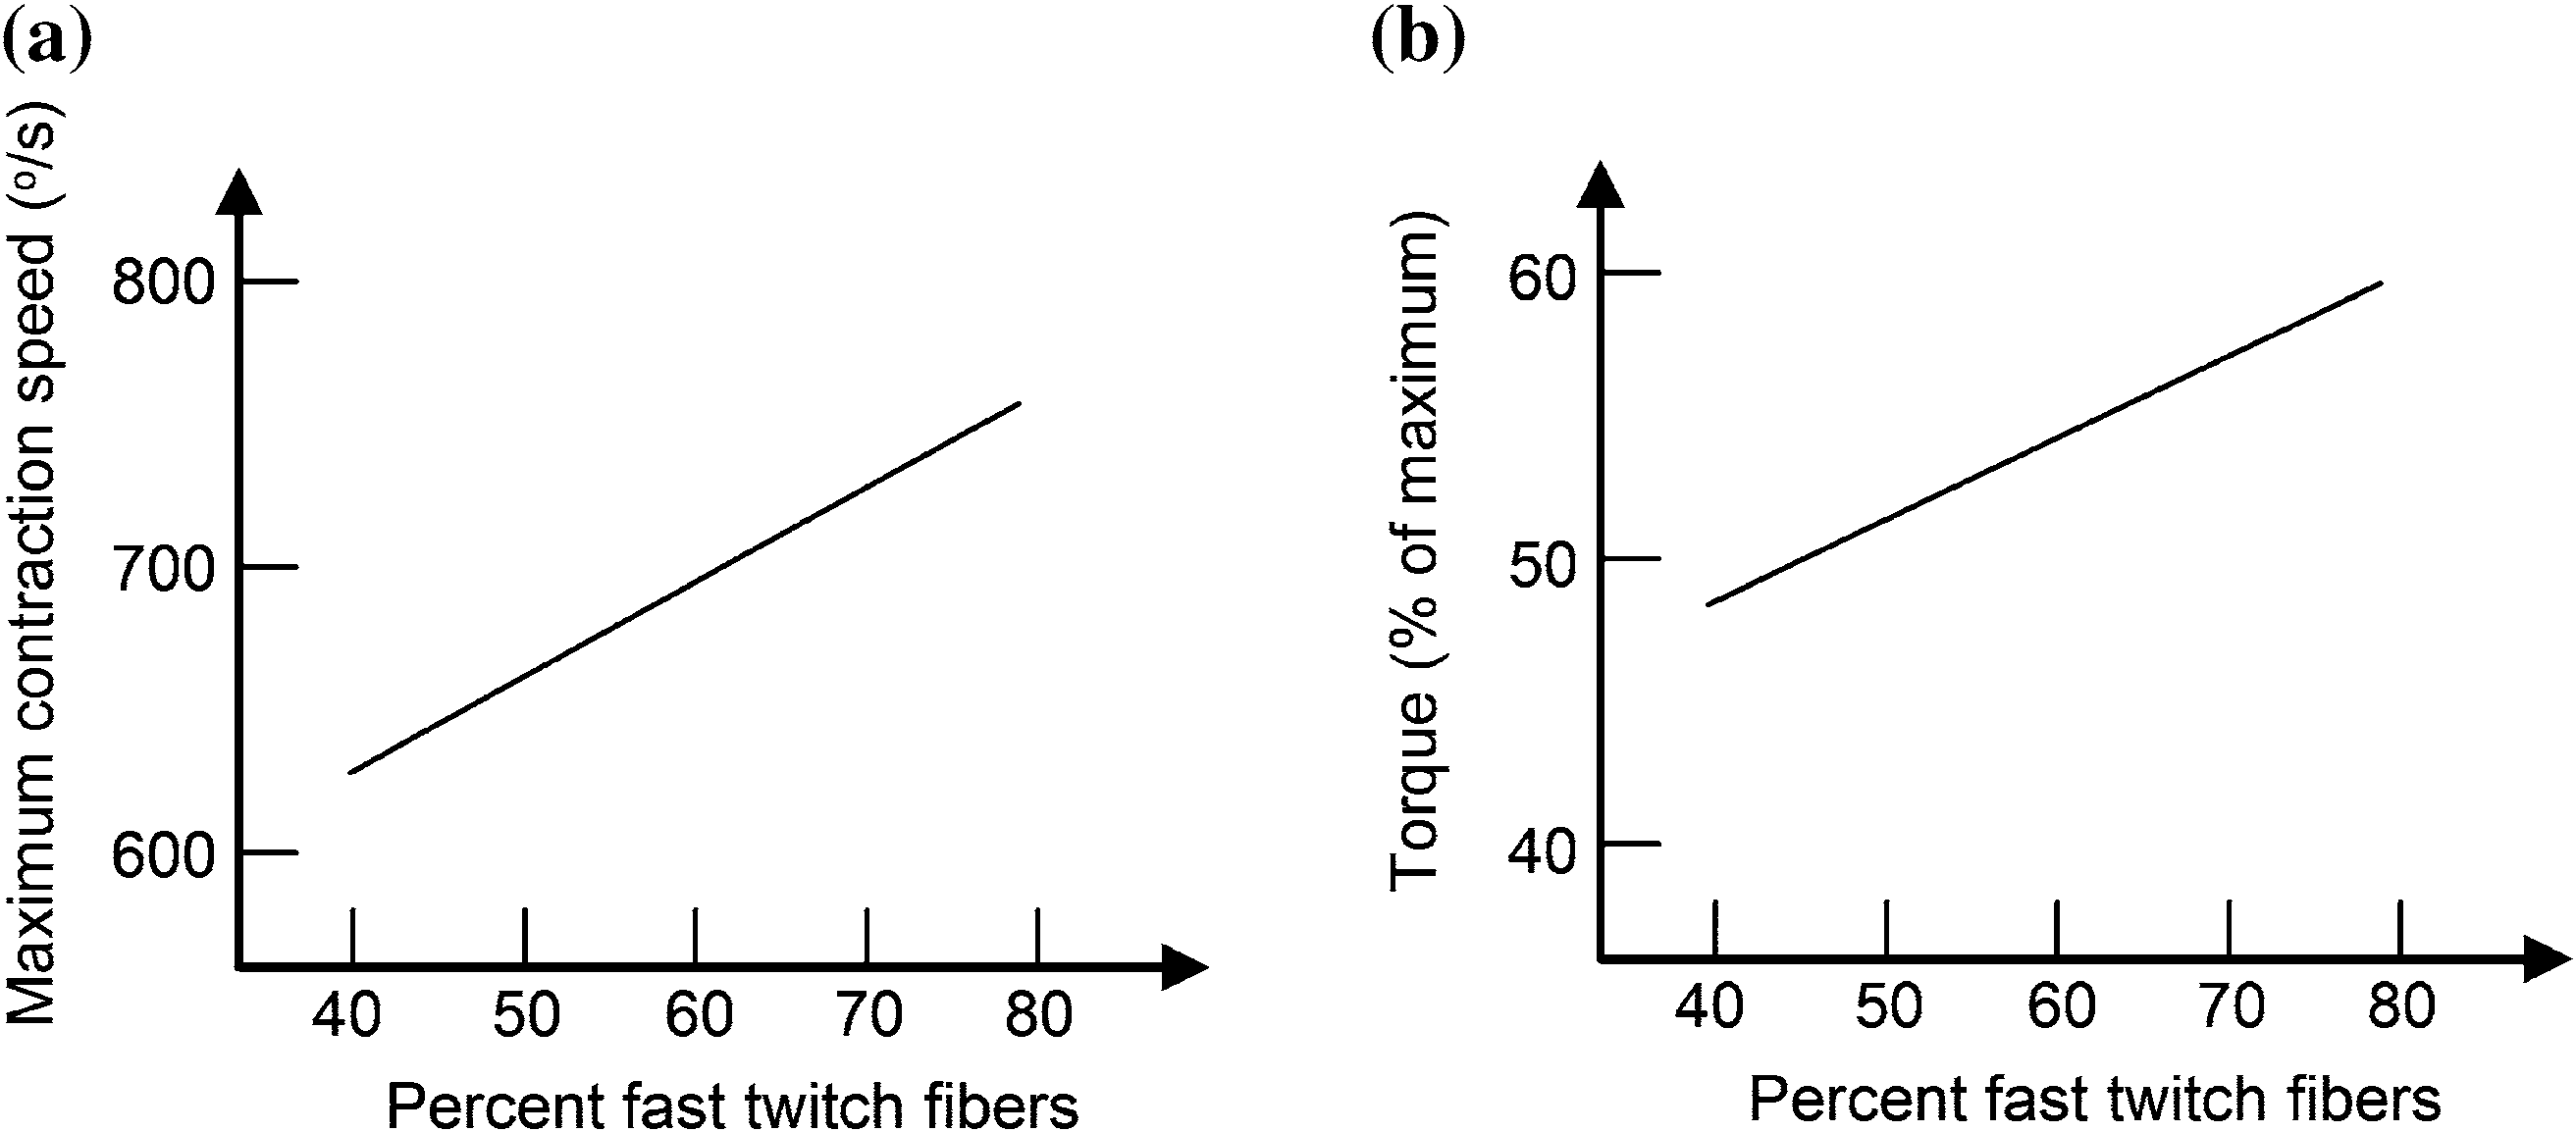
\includegraphics[width=0.8\textwidth]{512.png}
  \caption{Rendimiento de la extensión de la rodilla frente al porcentaje de fibras FT en la rodilla. (Basado en \cite{21} y \cite{73})}
  \label{fig:512}
\end{figure}



\subsection{Modelo mecánico del estado activo de los músculos}

Ahora desarrollamos un modelo macroscópico de los músculos en el estado activo debido a la estimulación eléctrica mediante el uso del tipo de modelos de resorte-amortiguador que empleamos para caracterizar la viscoelasticidad en el Cap. 4. Este modelo incluye resortes y amortiguadores para dar cuenta de las propiedades pasivas del músculo, y generadores de tensión para caracterizar el estado activo. Si bien caracteriza matemáticamente bastante bien las características mecánicas de los músculos esqueléticos que actúan contra cargas, los componentes individuales del modelo pueden o no describir las propiedades del músculo a nivel microscópico. Por ejemplo, la viscosidad representada por el amortiguador no modela muy bien el efecto de la viscosidad del fluido en un músculo. El elemento elástico en paralelo puede deberse, de hecho, al sarcolema, que es la membrana externa que rodea la fibra muscular. La proteína altamente elástica, titina (ver la Fig. 5.18 más abajo), forma una estructura similar a una red alrededor de los filamentos gruesos y delgados, y también puede contribuir a este elemento. Las regiones de bisagra de la miosina pueden contribuir a un elemento elástico en serie. (En el músculo cardíaco, se cree que el tejido conectivo es la parte principal del elemento elástico en paralelo).

\begin{table}[htbp]
\centering\footnotesize
\caption{Porcentajes de fibras musculares ST y FT en músculos seleccionados de atletas masculinos (M) y femeninos (F), junto con las áreas de sección transversal de estas fibras musculares}
\label{tab:58}
\begin{tabularx}{\textwidth}{Xcccccc}
\toprule
\textbf{Atleta} & \textbf{Género} & \textbf{Músculo} & \textbf{\%ST} & \textbf{\%FT} & \textbf{Área ST ($\mu\text{m}^2$)} & \textbf{Área FT ($\mu\text{m}^2$)} \\
\midrule
Corredores de velocidad & M & Gastrocnemio & 24 & 76 & 5.878 & 6.034 \\
 & F & Gastrocnemio & 27 & 73 & 3.752 & 3.930 \\
Corredores de fondo & M & Gastrocnemio & 79 & 21 & 8.342 & 6.485 \\
 & F & Gastrocnemio & 69 & 31 & 4.441 & 4.128 \\
Ciclistas & M & Vasto lateral & 57 & 43 & 6.333 & 6.116 \\
 & F & Vasto lateral & 51 & 49 & 5.487 & 5.216 \\
Nadadores & M & Deltoides posterior & 67 & 33 & -- & -- \\
Levantadores de pesas & M & Gastrocnemio & 44 & 56 & 5.060 & 8.910 \\
 & M & Deltoides & 53 & 47 & 5.010 & 8.450 \\
Triatletas & M & Deltoides posterior & 60 & 40 & -- & -- \\
 & M & Vasto lateral & 63 & 37 & -- & -- \\
 & M & Gastrocnemio & 59 & 41 & -- & -- \\
Piragüistas & M & Deltoides posterior & 71 & 29 & 4.920 & 7.040 \\
Lanzadores de peso & M & Gastrocnemio & 38 & 62 & 6.367 & 6.441 \\
No atletas & M & Vasto lateral & 47 & 53 & 4.722 & 4.709 \\
 & F & Gastrocnemio & 52 & 48 & 3.501 & 3.141 \\
\bottomrule
\end{tabularx}
\begin{flushleft}
    \small Obtenido de \cite{80}.
\end{flushleft}
\end{table}

La Figura 5.13a muestra un modelo mecánico con una unidad compuesta por un generador de tensión $T_0(x, t)$ en paralelo con un amortiguador de viscosidad $c$ y un resorte con constante de resorte $k_{\text{parallel}}$, que está en serie con otro resorte con constante de resorte $k_{\text{series}}$. La longitud total del músculo es $x_{\text{T}} = x_{\text{E}} + x$, donde $x_{\text{E}}$ es la longitud de equilibrio y $x$ es el desplazamiento.

\begin{figure}[htbp]
  \centering
  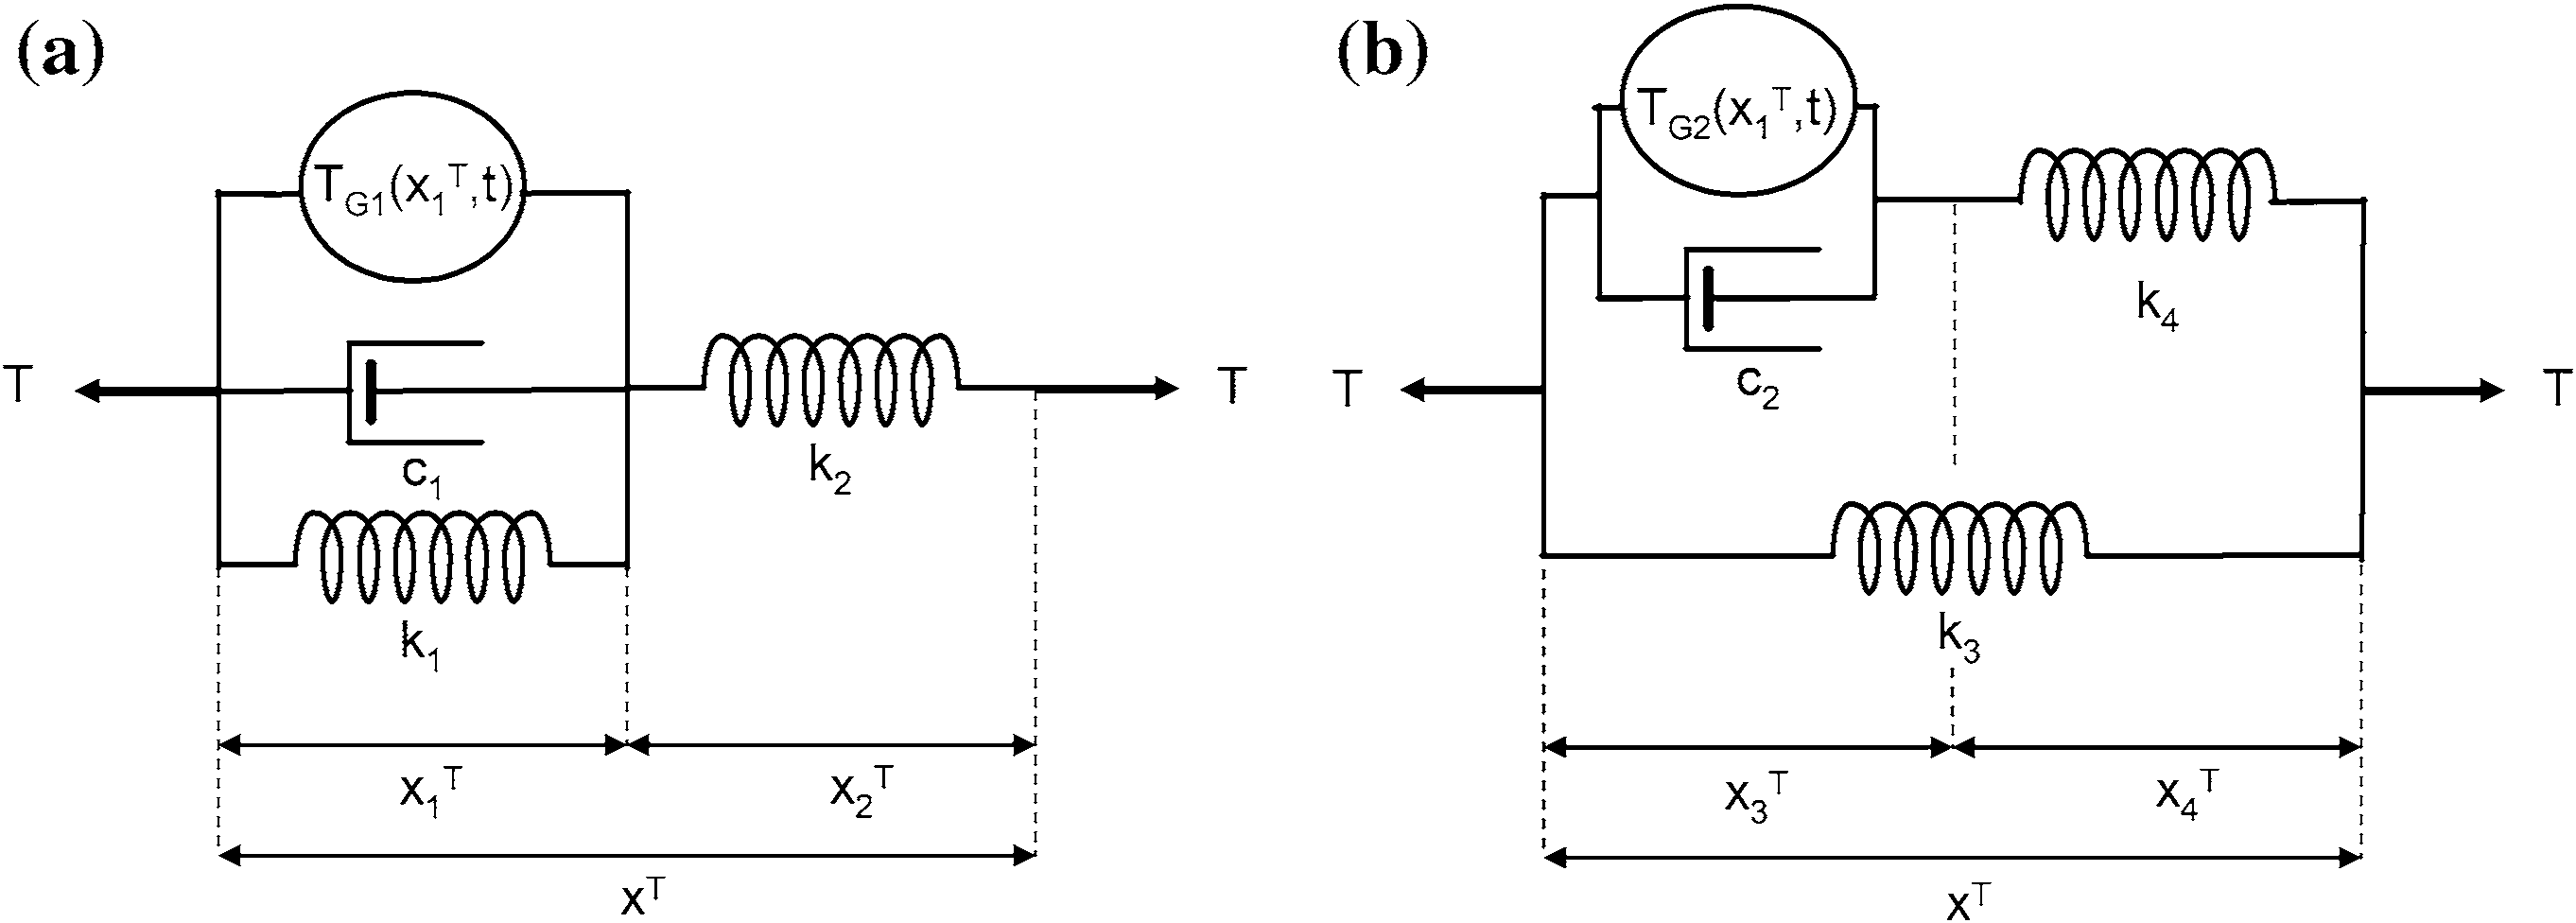
\includegraphics[width=0.8\textwidth]{513.png}
  \caption{Modelo completo del músculo en estado activo. (Basado en \cite{53})}
  \label{fig:513}
\end{figure}



Se puede demostrar que este modelo (el cual también se representa en la Fig. 5.14a) es matemáticamente equivalente al modelo mostrado en la Fig. 5.14b, en el cual hay una unidad con un resorte en serie con un generador de tensión en paralelo con un amortiguador, y esta unidad está en paralelo con otro resorte. Son matemáticamente equivalentes en el sentido de que las combinaciones de los componentes ofrecen las mismas predicciones del modelo. Las constantes de resorte y los coeficientes de viscosidad en los dos modelos no son iguales entre sí, pero están relacionados (ver el Problema 5.10). Esta representación del modelo en (a) es exactamente la misma que la del modelo de Kelvin / lineal estándar, excepto que el amortiguador está en paralelo con el generador de tensión.

\begin{figure}[htbp]
  \centering
  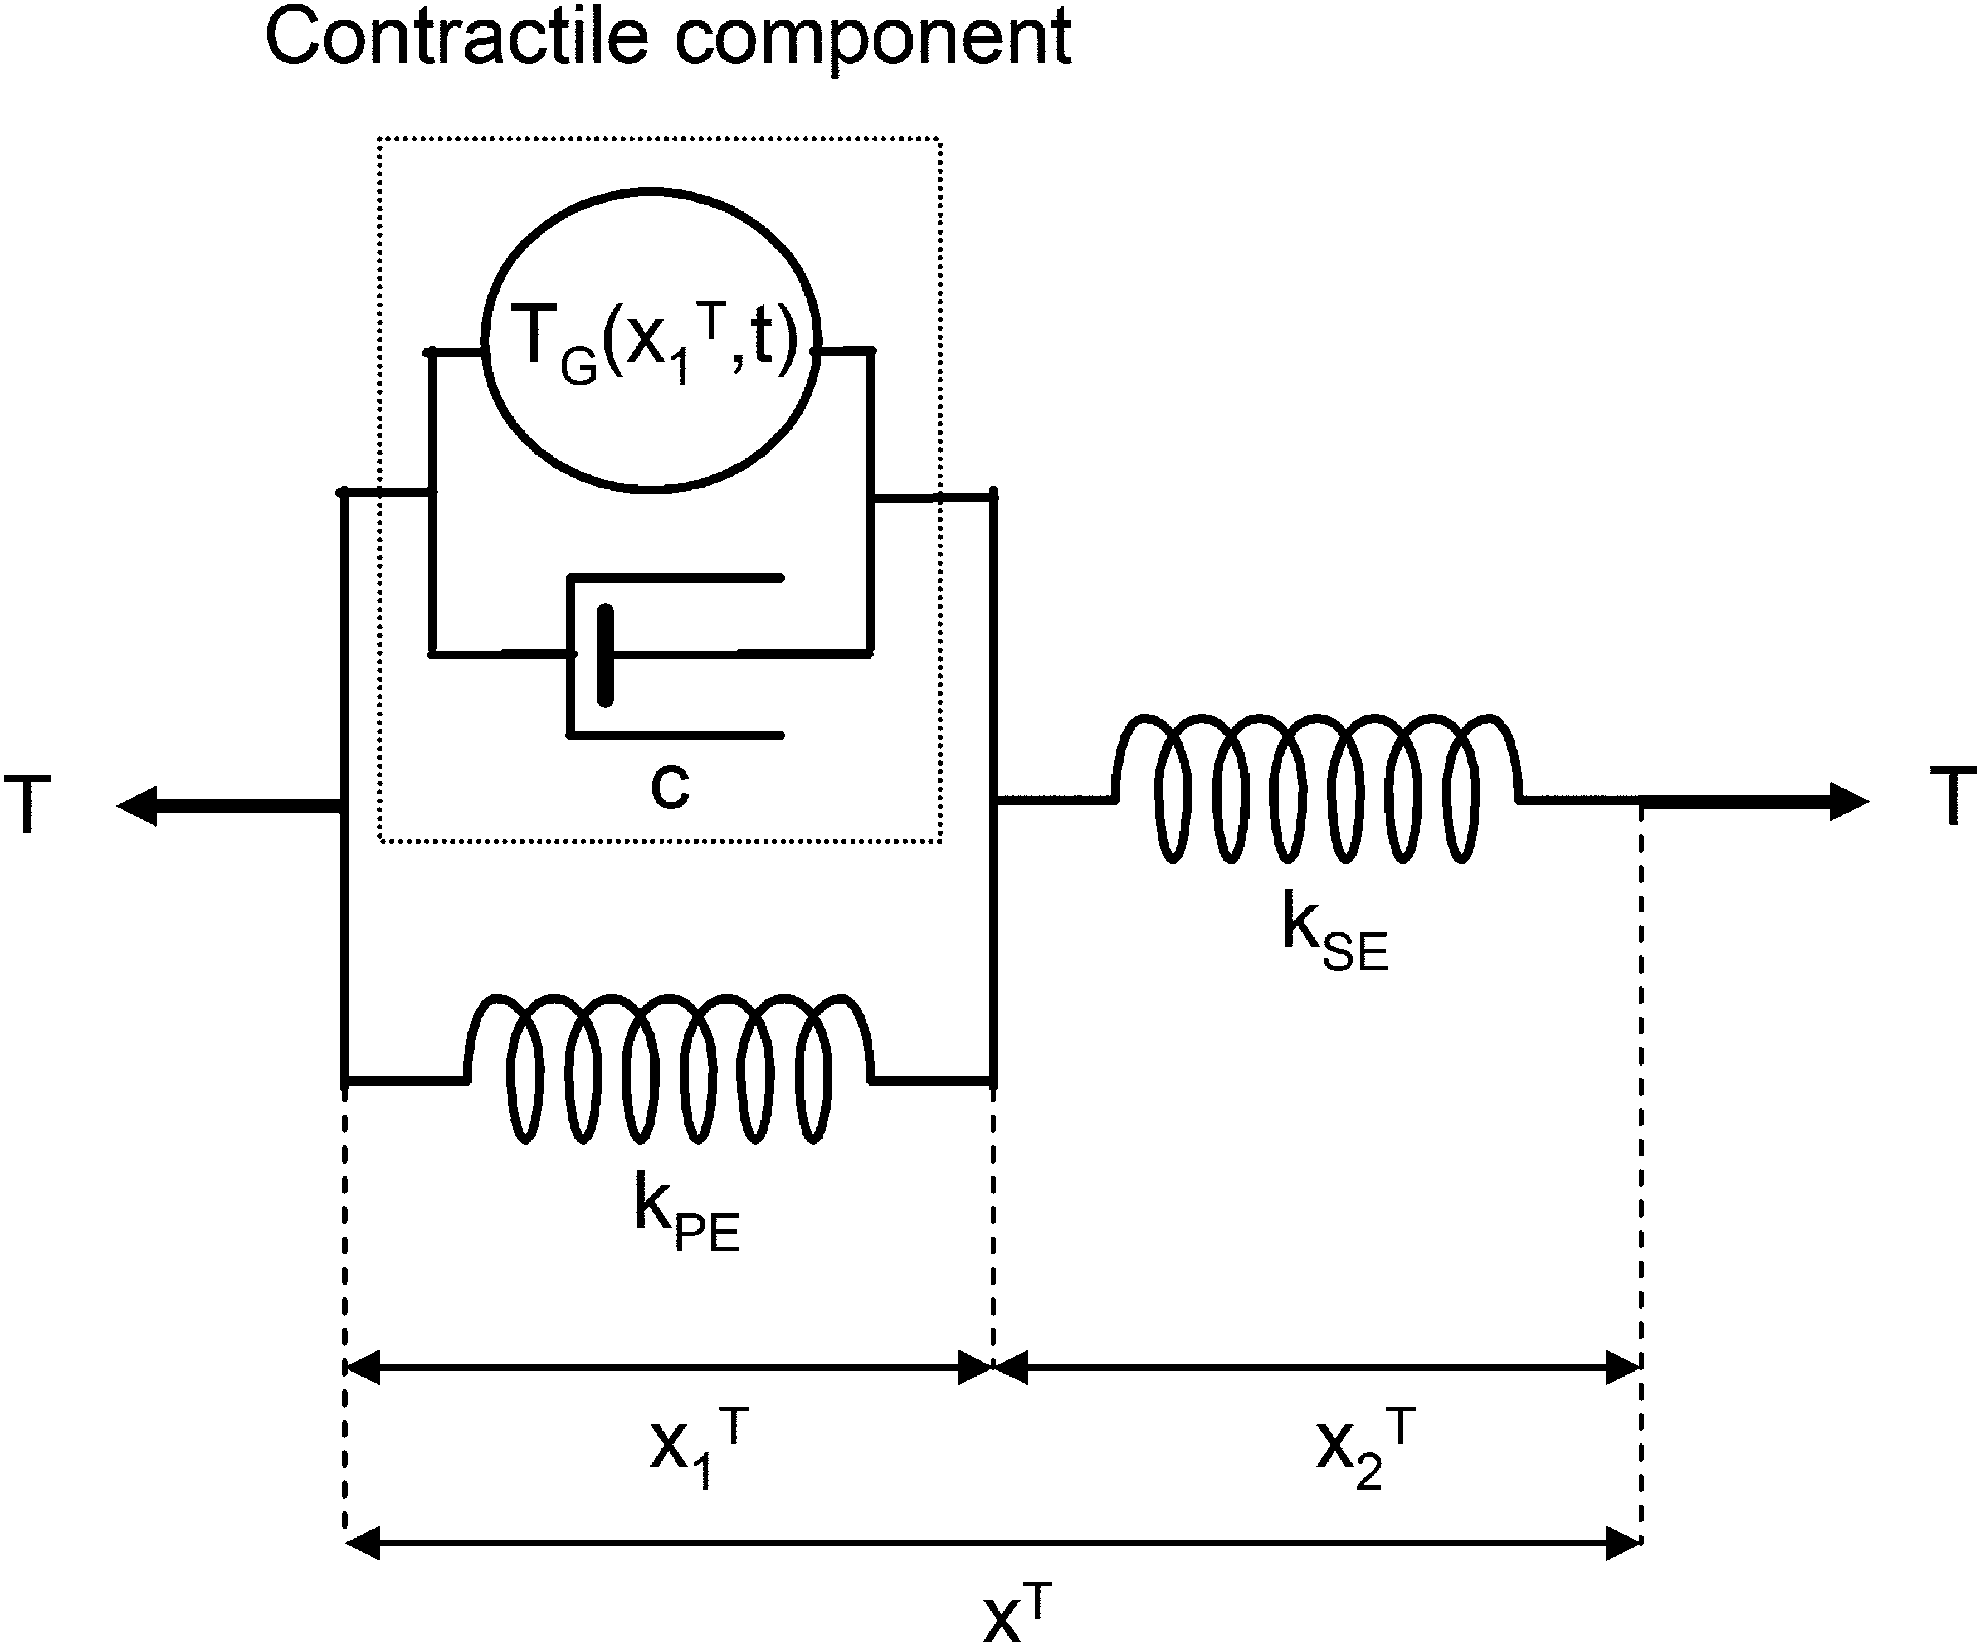
\includegraphics[width=0.7\textwidth]{514.png}
  \caption{Modelos equivalentes de músculo en estado activo. El modelo en la parte \textbf{a} es el mismo que el de la Fig. 5.13. (Basado en \cite{53})}
  \label{fig:514}
\end{figure}



Examinaremos el estado del músculo resolviendo un modelo ligeramente más simple, con solo el resorte con $k_{\text{series}}$ (ahora llamado $k$ por simplicidad) en la Fig. 5.15. Sin el generador de tensión, esto se reduce al modelo de Maxwell. El generador de tensión suministra una tensión que podría depender de la longitud del músculo $x$ y del tiempo $t$, $T_{\text{G}} = T_{\text{G}}(x, t)$.

\begin{SCfigure}[0.8][htbp]
  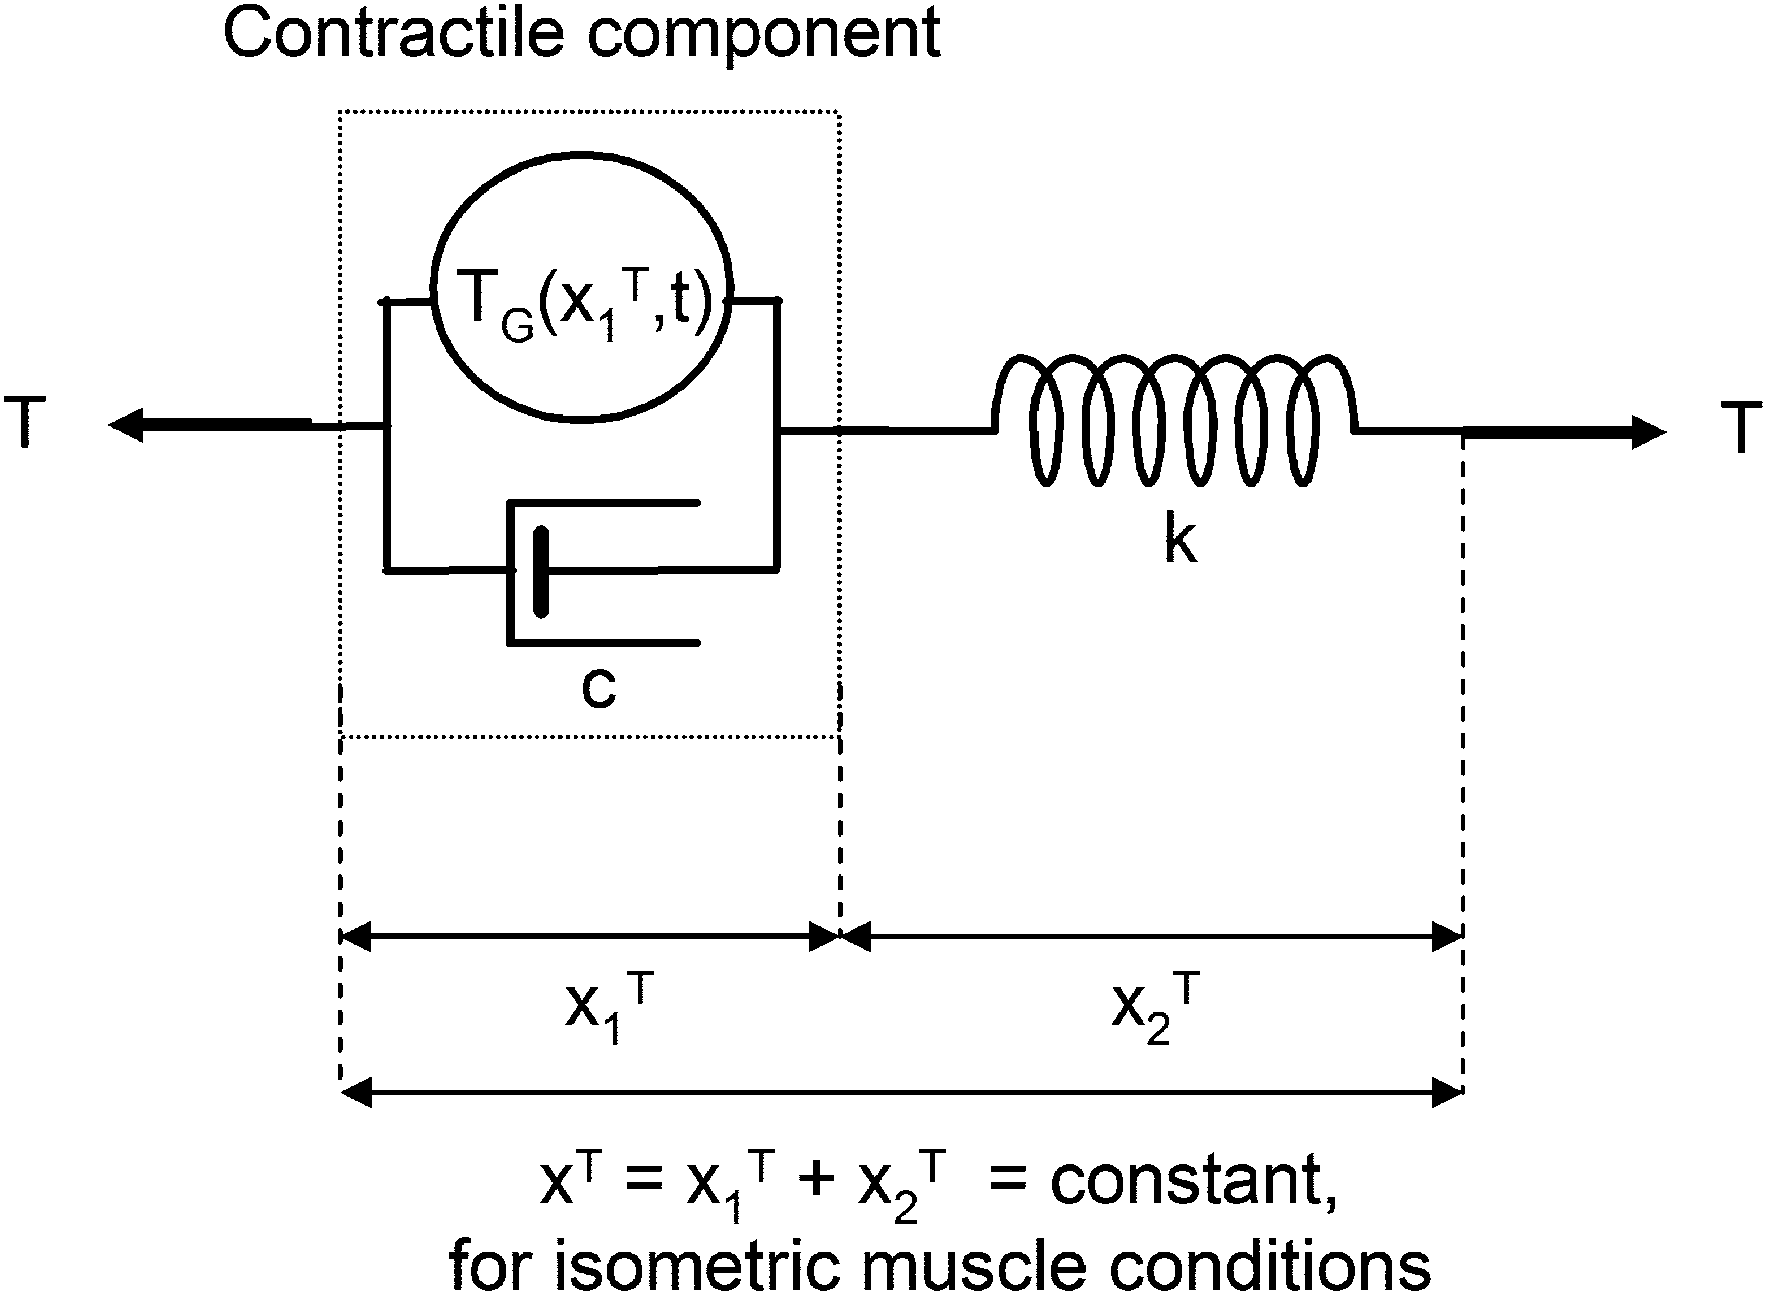
\includegraphics[width=0.55\textwidth]{515.png}
  \caption{Modelo más simple del músculo en estado activo. (Basado en \cite{53})}
  \label{fig:515}
\end{SCfigure}



% Control de Calidad: 8 párrafos origen -> 8 párrafos salida. Mapeo 1:1 verificado. Sin omisiones.

También asumiremos que la longitud total del músculo no cambia, es decir, condiciones isométricas. Esto significa que $x_{\text{T}} = x_{\text{T1}} + x_{\text{T2}}$ es constante, donde $x_{\text{T1}}$ es la longitud del amortiguador/generador de tensión y $x_{\text{T2}}$ es la longitud del resorte. Para condiciones isométricas, sabemos que $x(t) = 0$. Por consiguiente, el generador de tensión es $T_{\text{G}} = T_{\text{G}}(t)$. Diremos que este generador suministra la tensión $T_0$ durante periodos específicos de tiempo.

La longitud total del amortiguador/generador de tensión se puede subdividir en la longitud de equilibrio y el desplazamiento: $x_{\text{T1}} = x_{\text{E1}} + x_1$; para el resorte vemos que $x_{\text{T2}} = x_{\text{E2}} + x_2$. La fuerza generada a través del músculo es $T = T(t)$. Esta es igual a la tensión a través del resorte
\begin{equation}
T = kx_2,
\label{eq:5.2}
\end{equation}

y también es igual a la suma de las tensiones a través del generador de tensión y el amortiguador, por lo que
\begin{equation}
T = T_{\text{G}} + c \frac{dx_1}{dt}.
\label{eq:5.3}
\end{equation}

(Consúltese la discusión de los modelos de Maxwell y Voigt de la viscoelasticidad en el Cap. 4 para una explicación más detallada).

Debido a que $x_{\text{T}} = x_{\text{T1}} + x_{\text{T2}}$ es constante, vemos que $dx_{\text{T}}/dt = 0$. Además, como las distancias de equilibrio son constantes,
\begin{equation}
\frac{dx}{dt} = \frac{dx_1}{dt} + \frac{dx_2}{dt} = 0.
\label{eq:5.4}
\end{equation}
La ecuación (\ref{eq:5.3}) da $dx_1/dt = (T - T_{\text{G}})/c$ y la primera derivada de (\ref{eq:5.2}) da $dx_2/dt = (dT/dt)/k$, por lo que (\ref{eq:5.4}) se convierte en
\begin{equation}
\frac{T - T_{\text{G}}}{c} + \frac{1}{k} \frac{dT}{dt} = 0
\label{eq:5.5}
\end{equation}
o bien
\begin{equation}
\frac{dT(t)}{dt} + \frac{T(t)}{\tau} = \frac{T_{\text{G}}(t)}{\tau},
\label{eq:5.6}
\end{equation}
donde $\tau = c/k$ es el tiempo de relajación. $T(t)$ es una función de $t$ impulsada por $T_{\text{G}}(t)$.

La solución general para esto con $T_{\text{G}}(t) = \alpha$ (una constante) para $t > 0$ y $0$ para $t < 0$, con una tensión $T(0)$ en $t = 0$, es
\begin{equation}
T(t) = \alpha + (T(0) - \alpha) \exp(-t/\tau) = T(0) \exp(-t/\tau) + \alpha(1 - \exp(-t/\tau)).
\label{eq:5.7}
\end{equation}
Esto se puede demostrar sustituyendo esta expresión en (\ref{eq:5.6}) y verificando la solución en $t = 0$. (Ver el Apéndice C).

Antes de que se encienda el generador de tensión, $T_{\text{G}} = 0$ y $T(0) = 0$. En $t = 0$, $T_{\text{G}}(t) = T_0 (= \alpha)$ durante un periodo de tiempo, tiempo durante el cual (\ref{eq:5.7}) es
\begin{equation}
T(t) = T_0(1 - \exp(-t/\tau)),
\label{eq:5.8}
\end{equation}
como se muestra en la Fig. 5.16a.

Si el generador de tensión se apaga al tiempo $t_1$, de modo que $T_{\text{G}}(t) = 0$ para $t > t_1$, entonces la tensión existente en $t_1$ es
\begin{equation}
T(t_1) = T_0(1 - \exp(-t_1/\tau)),
\label{eq:5.9}
\end{equation}
y (\ref{eq:5.7}) (ahora con $\alpha = 0$) muestra que la tensión decae a una tasa de $\exp(-\Delta t/\tau)$, donde $\Delta t = t - t_1$. Por lo tanto, para $t > t_1$,
\begin{equation}
T(t) = T_0(1 - \exp(-t_1/\tau)) \exp(-(t - t_1)/\tau),
\label{eq:5.10}
\end{equation}
como se observa en la Fig. 5.16b.

Este es el modelo de una sola sacudida. Podemos considerar secuencias de dos sacudidas separadas en el tiempo una justo después de la otra (ver la Fig. 5.16c). Digamos que la activación está apagada durante un tiempo $t_2$ y se enciende de nuevo en $t_1 + t_2$ durante un tiempo $t_1$ (hasta $2t_1 + t_2$). Entonces la tensión al inicio de la segunda sacudida es
\begin{equation}
T(t_1 + t_2) = T_0(1 - \exp(-t_1/\tau)) \exp(-t_2/\tau).
\label{eq:5.11}
\end{equation}
Para $t_1 + t_2 < t < 2t_1 + t_2$, la tensión evoluciona como se indica en (\ref{eq:5.7}), utilizando (\ref{eq:5.11}) para la tensión inicial, $\alpha = T_0$, y reemplazando $t$ por $t - (t_1 + t_2)$ en el lado derecho de la ecuación (lo cual es una nueva definición del tiempo de inicio). Por lo tanto,
\begin{equation}
T(t) = T_0\{1 + [\exp(-t_2/\tau) - \exp(-(t_1 + t_2)/\tau) - 1] \exp(-(t - (t_1 + t_2))/\tau)\}
\label{eq:5.12}
\end{equation}
\begin{equation}
= T_0\{1 - \exp(-t/\tau) + \exp(-(t - t_1)/\tau) - \exp(-(t - (t_1 + t_2))/\tau)\}.
\label{eq:5.13}
\end{equation}

\begin{figure}[htbp]
  \centering
  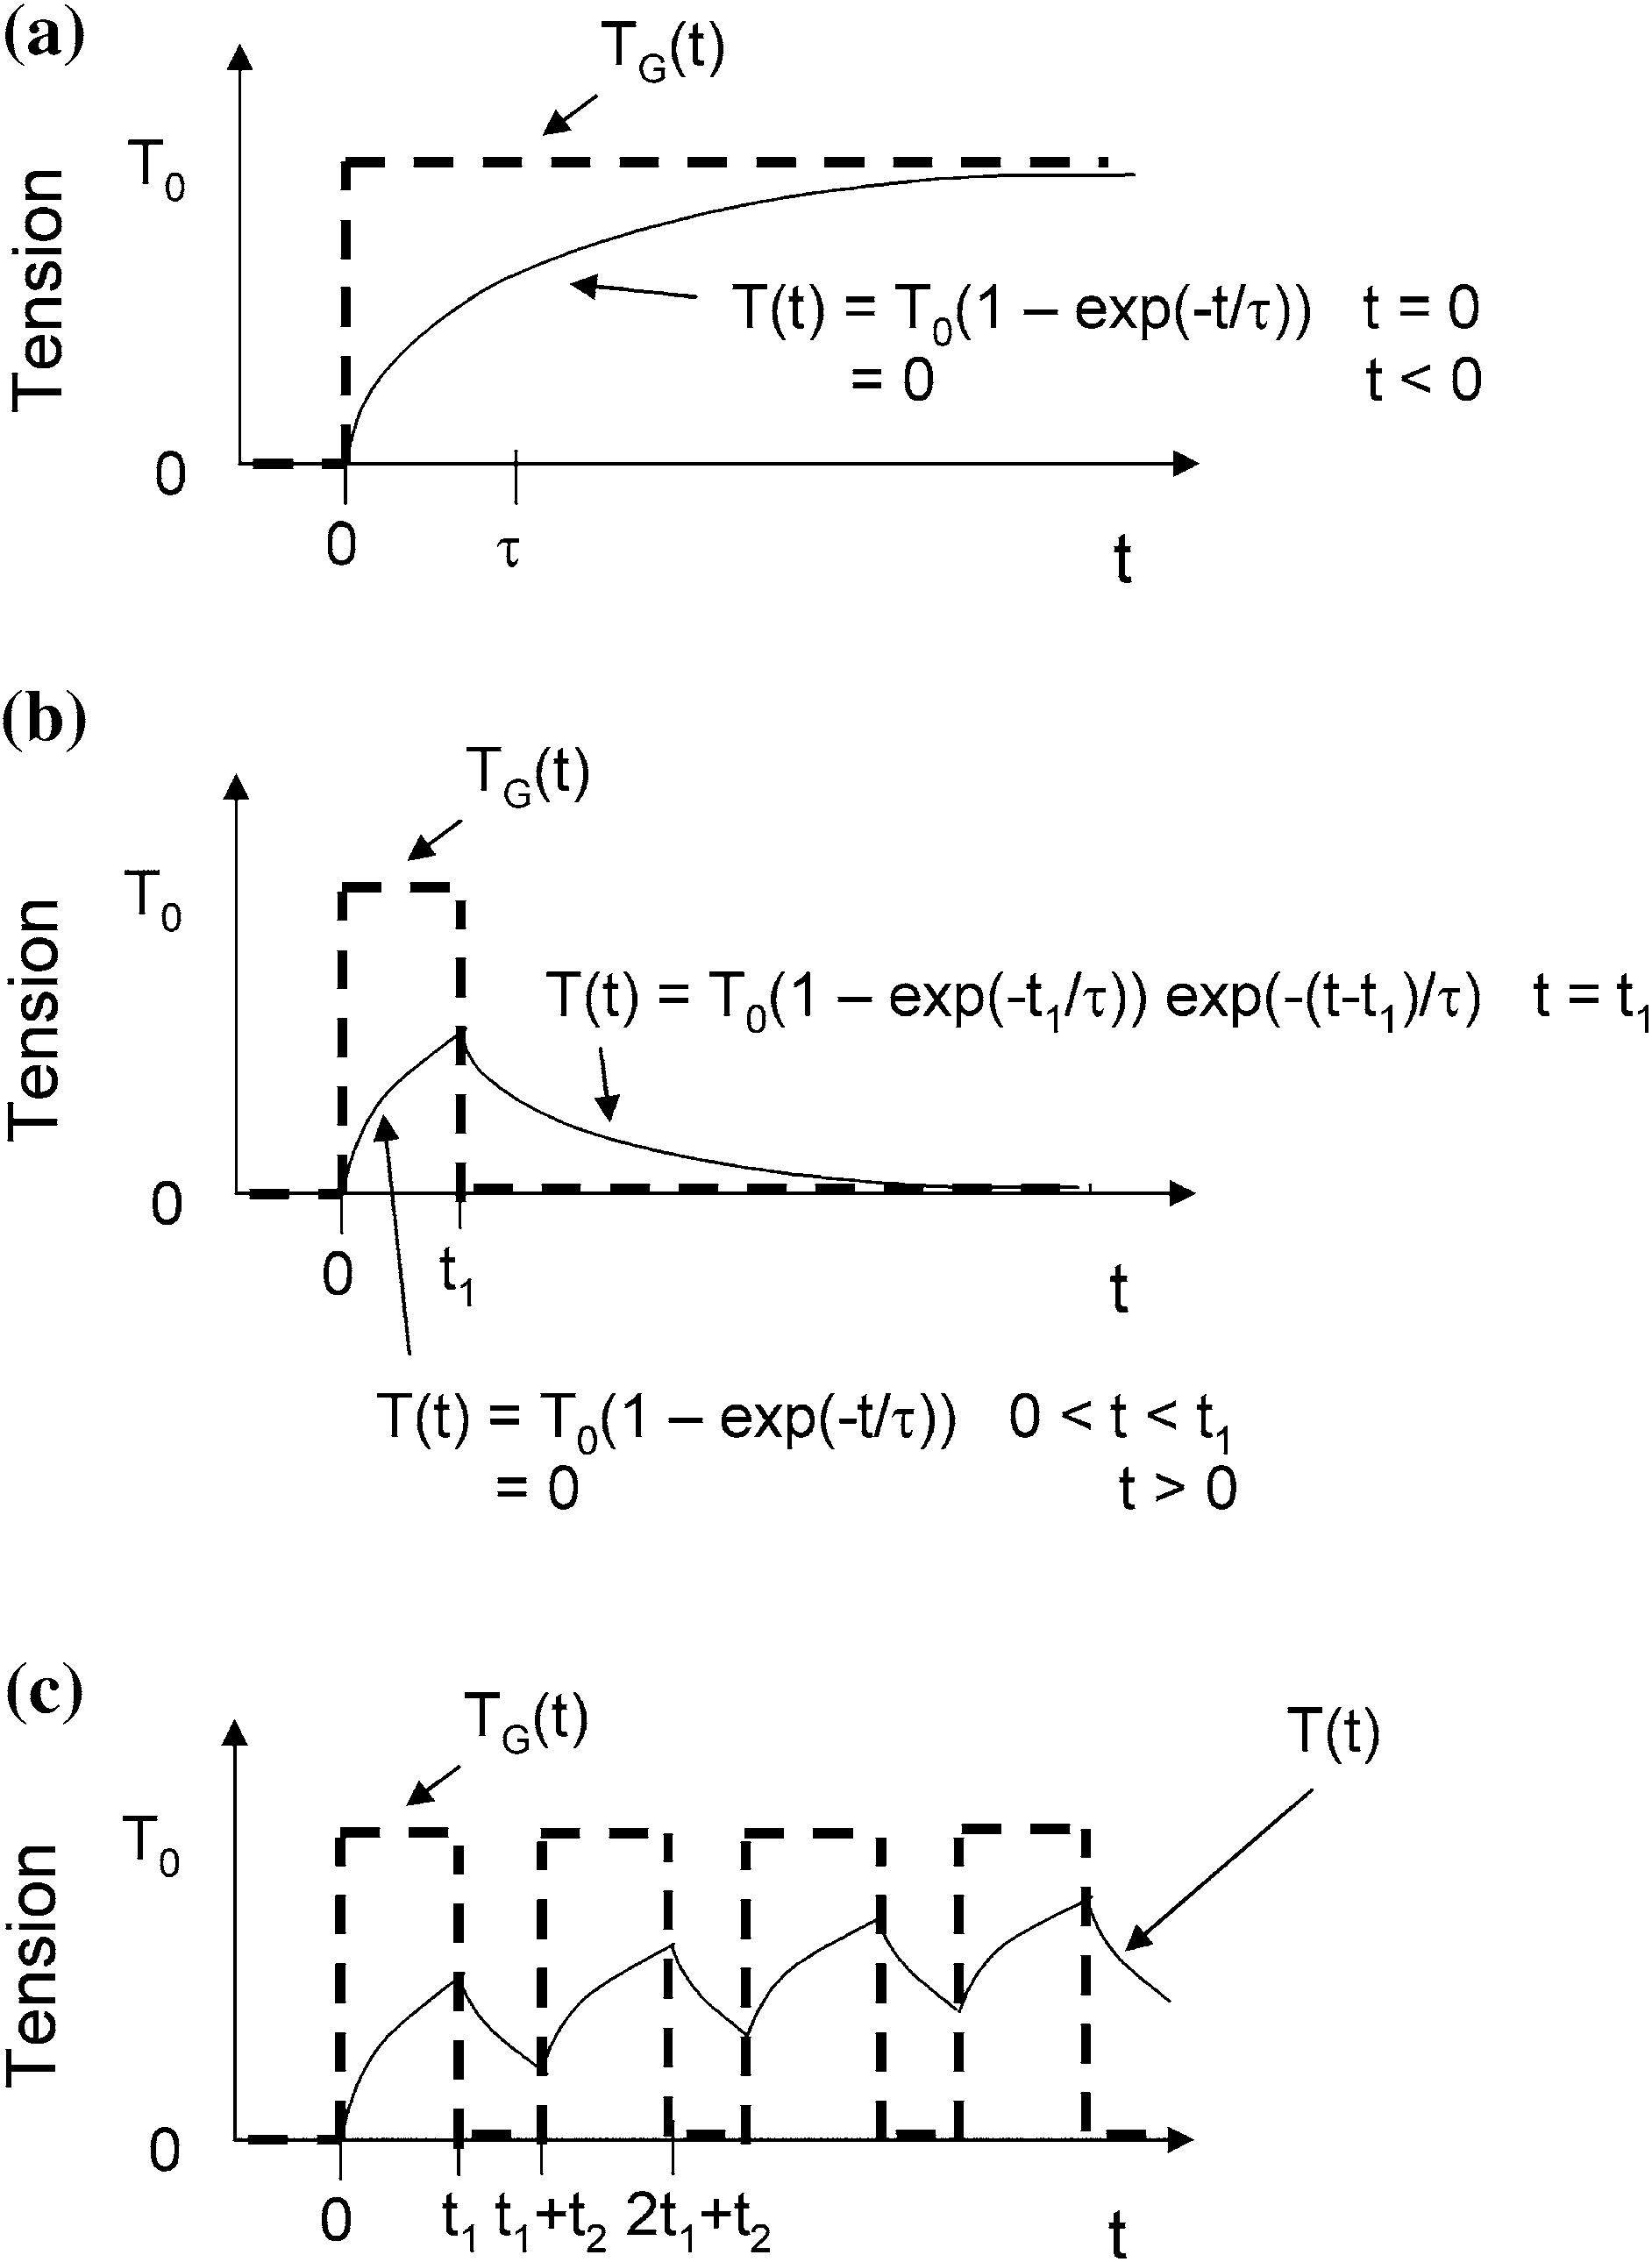
\includegraphics[width=0.45\textwidth]{516.png}
  \caption{Soluciones del modelo de músculo en estado activo de la Fig. 5.15 para la tensión con excitación por \textbf{a} una función escalón, \textbf{b} un pulso cuadrado y \textbf{c} una onda cuadrada. El texto deriva la solución después de dos pulsos cuadrados secuenciales al tiempo $2t_1 + t_2$ en \textbf{c}. (Basado en \cite{53})}
  \label{fig:516}
\end{figure}



Al final de la segunda sacudida $t = 2t_1 + t_2$, por lo que
\begin{equation}
T(t) = T_0\{1 - \exp(-(2t_1 + t_2)/\tau) + \exp(-(t_1 + t_2)/\tau) - \exp(-t_1/\tau)\}
\label{eq:5.14}
\end{equation}
\begin{equation}
= T_0[1 - \exp(-t_1/\tau)][1 + \exp(-(t_1 + t_2)/\tau)],
\label{eq:5.15}
\end{equation}
lo cual es $(1 + \exp(-(t_1 + t_2)/\tau))\times$ mayor que al final de la primera sacudida.

Al final de $N$ de tales sacudidas, la tensión es mayor que al final de la primera sacudida por un factor de $1 + \exp(-(t_1+t_2)/\tau) + \exp(-2(t_1+t_2)/\tau) + \dots + \exp(-N(t_1+t_2)/\tau)$, el cual para un valor de $N$ grande se aproxima a $1 / [1 - \exp(-(t_1 + t_2)/\tau)]$. (La suma geométrica $1 + x + x^2 + x^3 + \dots \to 1/(1 - x)$ para $0 < x < 1$). Por lo tanto, la tensión total desarrollada en el estado tetanizado es
\begin{equation}
T_{\text{tetanized}} = T_0 \frac{1 - \exp(-t_1/\tau)}{1 - \exp(-(t_1 + t_2)/\tau)}.
\label{eq:5.16}
\end{equation}
Si los pulsos se suceden inmediatamente uno detrás del otro, de modo que $t_2 = 0$, esta ecuación se convierte en $T_{\text{tetanized}} = T_0$, lo cual tiene sentido.

La Figura 5.17 muestra un modelo mecánico más completo de un músculo, con sarcómeros individuales modelados.

\begin{figure}[htbp]
  \centering
  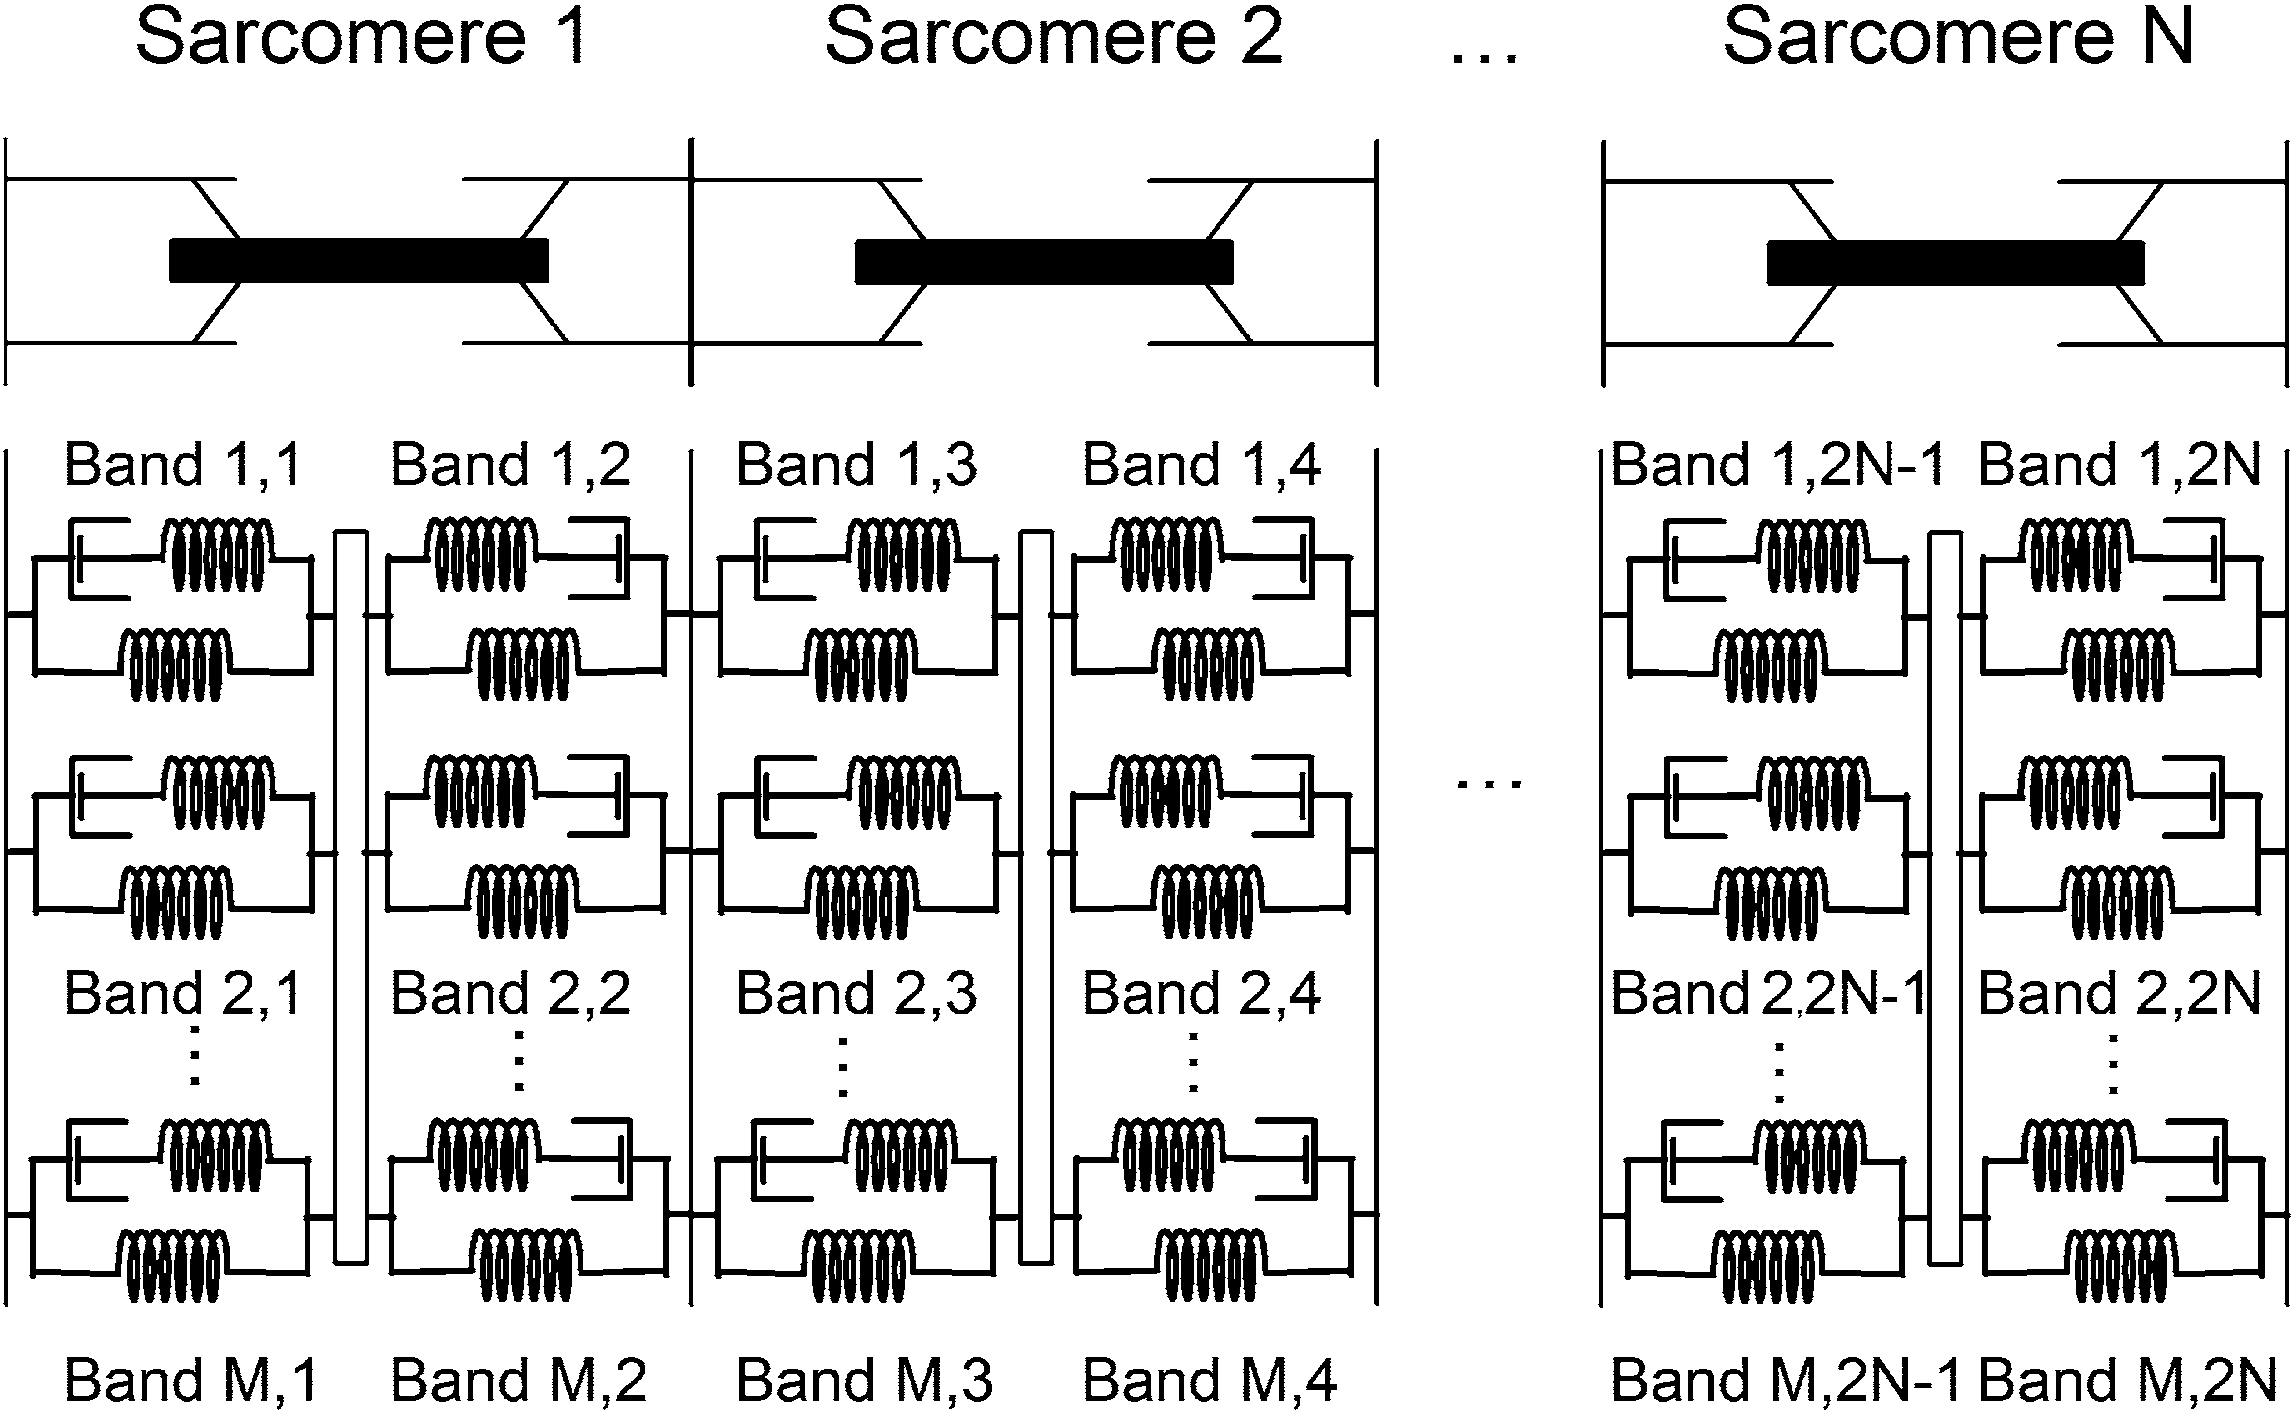
\includegraphics[width=0.8\textwidth]{517.png}
  \caption{Diagrama esquemático de una fibra muscular constituida por los modelos más simples. Este modelo de músculo más completo está construido a partir de una red distribuida de $N$ sarcómeros. (Basado en \cite{15} y \cite{61})}
  \label{fig:517}
\end{figure}



\section{Músculos pasivos}

Un músculo pasivo o en reposo sin estimulación eléctrica tiene propiedades mecánicas que deben comprenderse como parte de la exploración del estado activo del músculo, debido a que afectan el rendimiento muscular durante la activación. Experimentalmente se encuentra que los músculos pasivos son no Hookeanos, como en (4.22). La ecuación (4.27) mostró que para deformaciones mayores, la tensión y la deformación se relacionan por
\begin{equation}
\sigma = \mu' \exp(\alpha L/L_0) - \mu,
\label{eq:5.17}
\end{equation}
siendo $\lambda = L/L_0 = \epsilon + 1$ la deformación lagrangiana, donde $L$ es la longitud del músculo y $L_0$ es la longitud relajada.

Utilizando esto, la fuerza a través de un músculo pasivo se relaciona con la tensión mediante
\begin{equation}
F_{\text{M}} = \sigma(\text{PCA}).
\label{eq:5.18}
\end{equation}
Por consiguiente, la fuerza necesaria para mantener un músculo pasivo a una longitud $L$ es
\begin{equation}
F_{\text{M}} = (\text{PCA})\mu' \exp(\alpha L/L_0) - (\text{PCA})\mu.
\label{eq:5.19}
\end{equation}
Para grandes deformaciones, se necesitan utilizar relaciones más generales para este régimen neo-Hookeano y para definir las deformaciones. El Capítulo 4 y los Problemas 4.20--4.22 explican esto con mayor detalle.

% Control de Calidad: 14 párrafos origen -> 14 párrafos salida. Mapeo 1:1 verificado. Sin omisiones.

\section{Músculos activos/tetanizados: perspectiva microscópica}

A diferencia de las partes pasivas de los órganos cuyas longitudes cambian debido a las tensiones aplicadas, las longitudes de los músculos cambian y la fuerza se genera por el deslizamiento de los filamentos gruesos sobre los filamentos delgados, como se observa en las Figs. 5.18 y 5.19. Debido a que la unidad funcional básica que experimenta este movimiento es el sarcómero, el cual mide $\sim 2\ \mu\text{m}$ de largo, estas figuras describen una perspectiva microscópica de la acción muscular.

\begin{figure}[htbp]
  \centering
  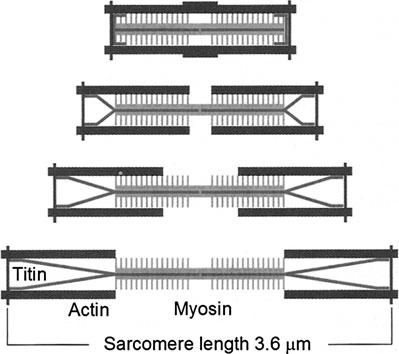
\includegraphics[width=0.7\textwidth]{518.png}
  \caption{Esquema del mecanismo de filamentos deslizantes en los sarcómeros, con deslizamiento relativo de los filamentos gruesos y delgados, para sarcómeros de longitud creciente: $1,6$, $2,2$, $2,9$ y $3,6\ \mu\text{m}$ (que se corresponden aproximadamente con los sarcómeros destacados en la Fig. 5.19). Nótese que el material elástico titina se muestra esquemáticamente conectando el filamento grueso a la estructura; desempeña un papel importante en las propiedades elásticas de los músculos. Ver también la Fig. 5.35. (De \cite{68})}
  \label{fig:518}
\end{figure}



La fuerza de tensión máxima que puede ser desarrollada por un músculo depende de varias magnitudes, incluyendo la longitud actual del músculo, la tasa actual de contracción muscular y el área de sección transversal fisiológica ($\text{PCA}$) del músculo. Bajo condiciones óptimas, esta fuerza es de $\sim 30\text{ N/cm}^2$ para muchos músculos en la mayoría de los mamíferos.

La tensión generada por un músculo cuando sus dos extremos se mantienen fijos, lo que se denomina condiciones isométricas, se muestra en la Fig. 5.19. La fuerza máxima generada por un músculo ocurre a la longitud óptima $L_0$. (Esto ocurre a una longitud muscular ligeramente mayor que la longitud inicial o de reposo $L_{\text{i}}$, antes de la activación). Este nivel máximo de fuerza disminuye a la mitad de este valor cuando la longitud del músculo es el $70\%$ (músculo acortado) o el $130\%$ (músculo alargado) de esta longitud óptima. Es casi cero al $170\%$ de esta longitud de reposo. Estas observaciones se refieren tanto a la longitud total del músculo real como a la longitud de cada sarcómero de $\sim 2\ \mu\text{m}$ de largo \cite{12}.

\begin{figure}[htbp]
  \centering
  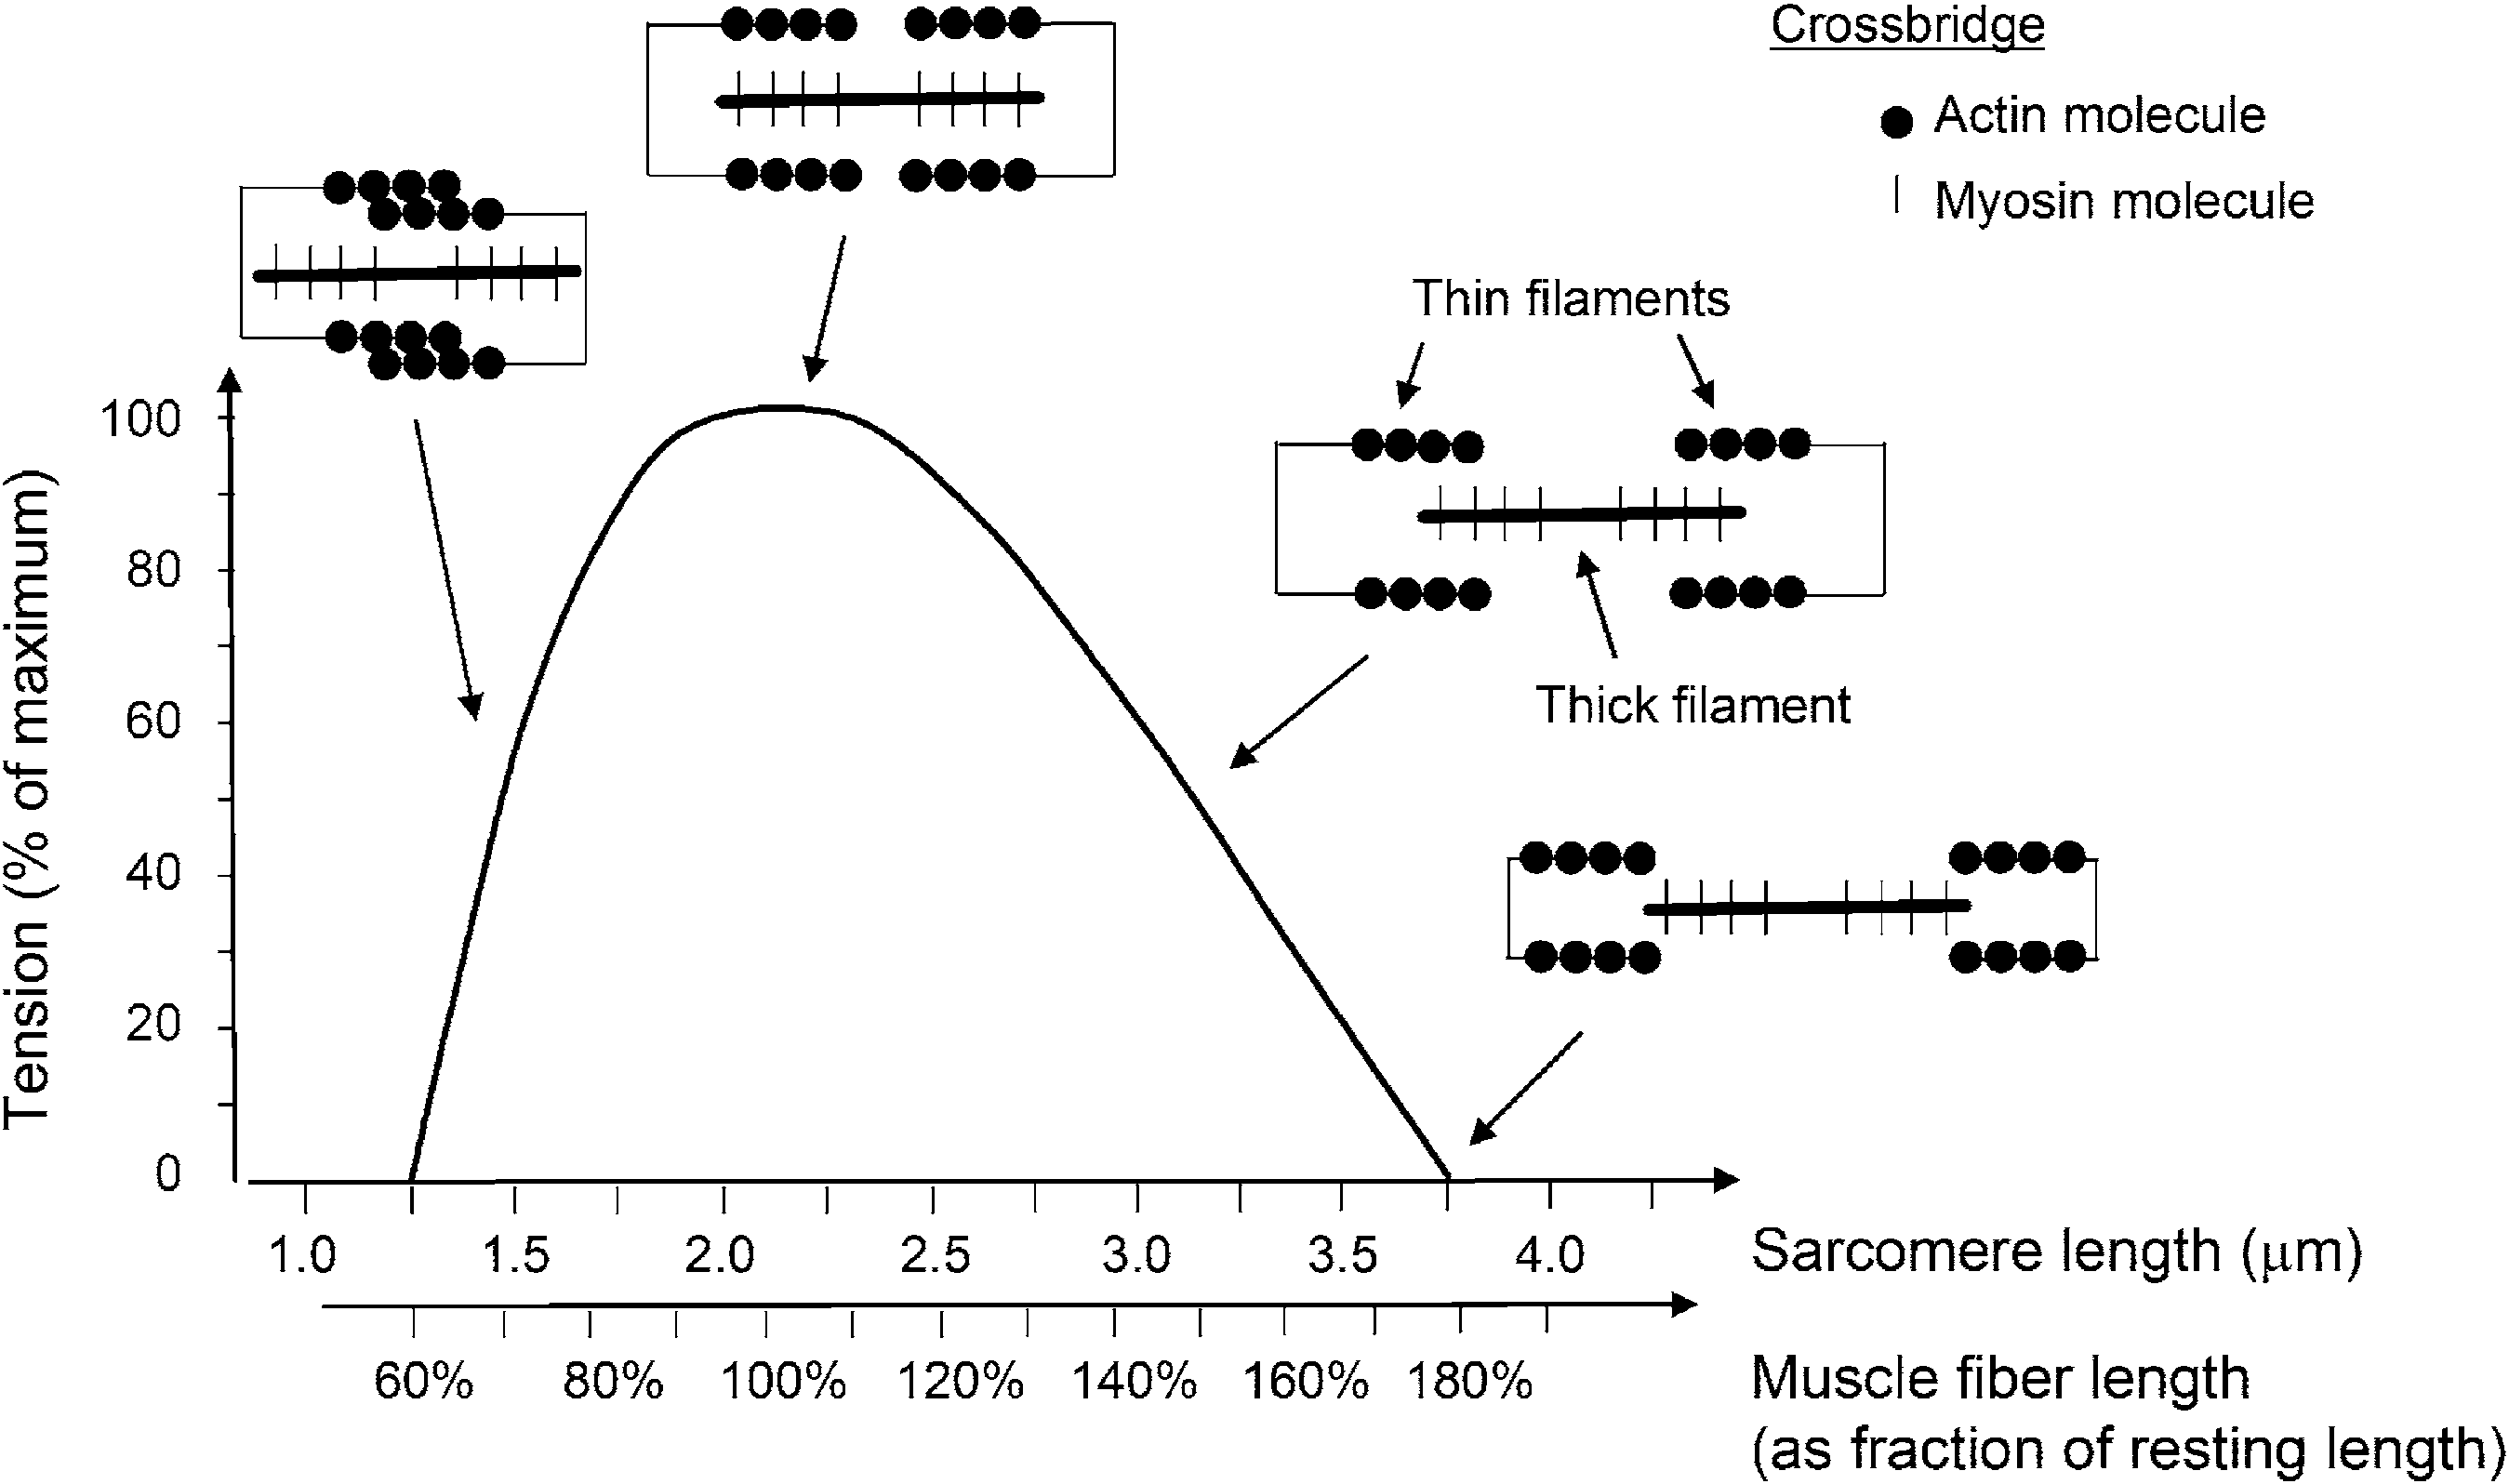
\includegraphics[width=0.8\textwidth]{519.png}
  \caption{Fuerza frente a la longitud del sarcómero o del músculo, con esquemas de la variación de la superposición de los filamentos gruesos (miosina) y delgados (actina) para diferentes longitud de sarcómero. Las longitudes del sarcómero y del músculo total escalan de la misma manera. También se muestra el puente cruzado entre una molécula de actina y una de miosina. (Basado en \cite{26, 53, 67, 71})}
  \label{fig:519}
\end{figure}



La base física de esta tensión es el grado de superposición de las moléculas de miosina y actina en los filamentos gruesos y delgados. A la longitud de reposo, el número de superposiciones de pares de miosina/actina es máximo, y este número de pares superpuestos disminuye cuando el sarcómero se acorta o se alarga. Estas interacciones de estos pares de moléculas se conocen como puentes cruzados entre los filamentos gruesos y delgados.

Una consecuencia de cambiar la longitud del músculo es el cambio concomitante en el ángulo de la articulación (Problema 5.16). Por consiguiente, la fuerza generada y el torque resultante también dependen del ángulo de la articulación. La Figura 5.20 muestra la fuerza frente al ángulo de la articulación para varias articulaciones.

\begin{figure}[htbp]
  \centering
  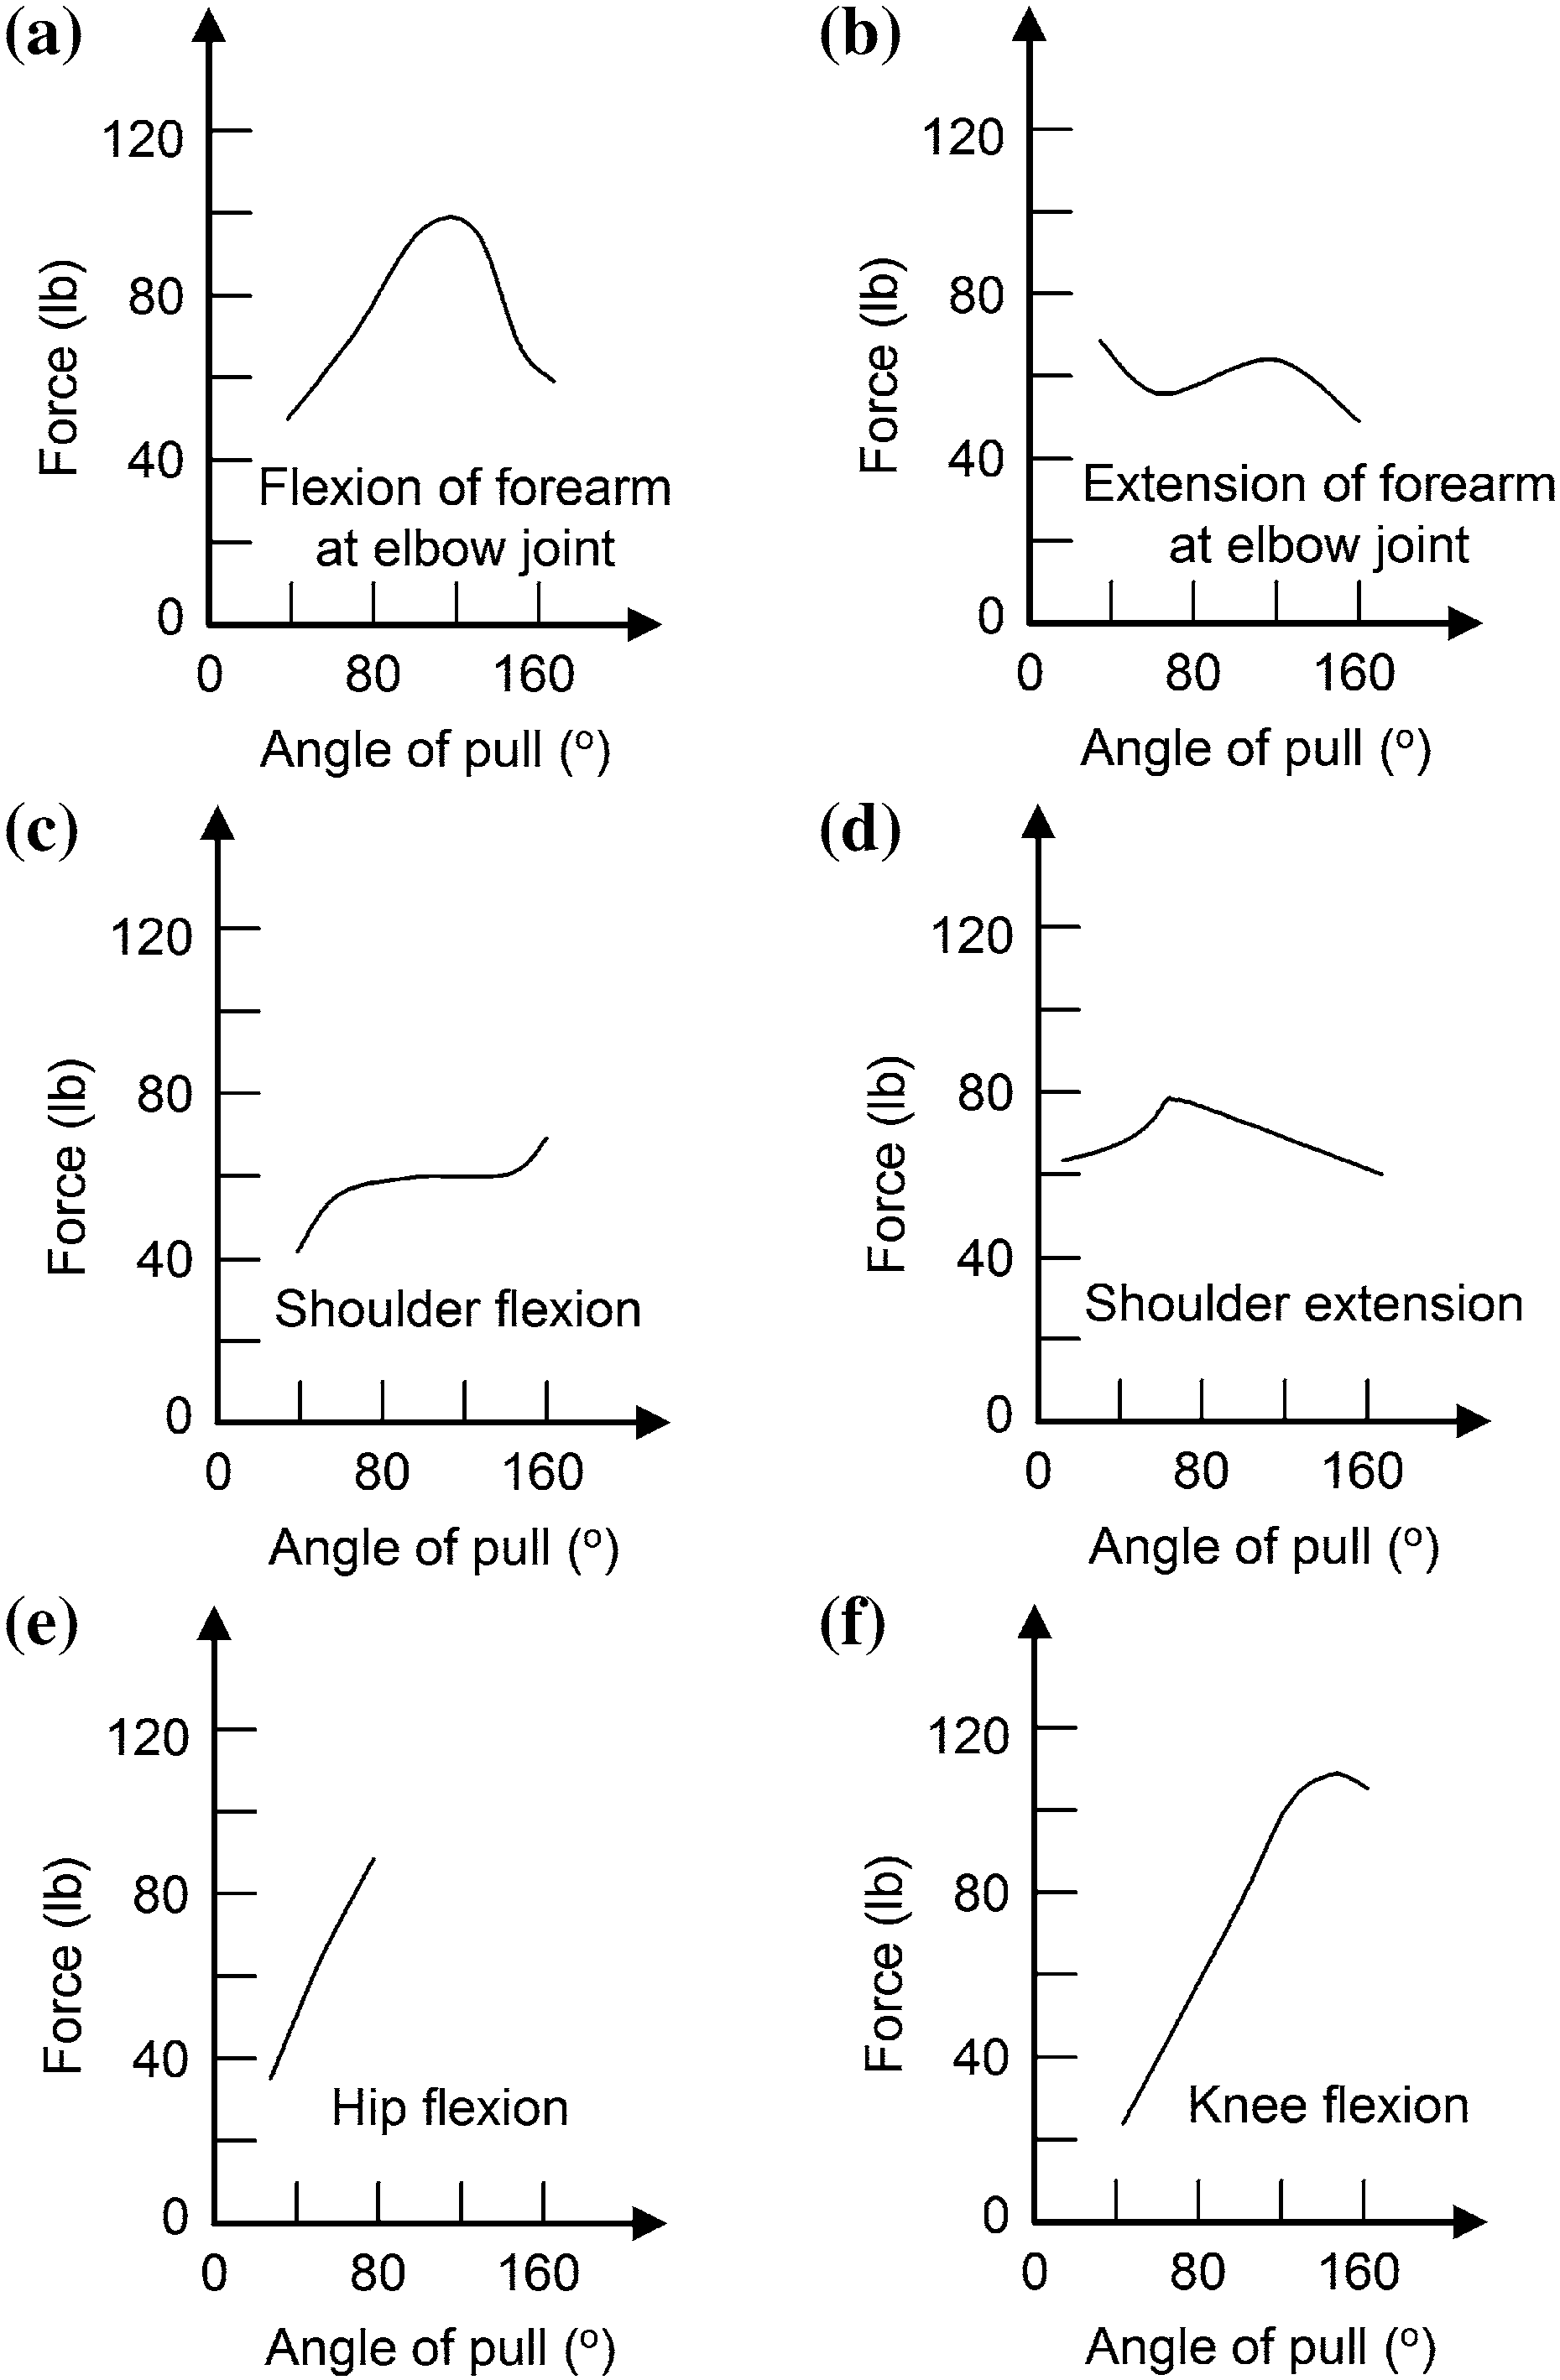
\includegraphics[width=0.45\textwidth]{520.png}
  \caption{Fuerza frente al ángulo para la flexión y extensión del codo y del hombro, y la flexión de la cadera y la rodilla. Solo algunos de estos gráficos se parecen al perfil clásico de fuerza frente a longitud (Fig. 5.19, convertido en un gráfico frente al ángulo de la articulación) para una sola fibra muscular o sarcómero. (Basado en \cite{20})}
  \label{fig:520}
\end{figure}



\subsection{Tensión muscular total}

La Figura 5.21 muestra la tensión tetanizada total frente a la longitud del músculo. Claramente se ve diferente a la respuesta mostrada en la Fig. 5.19. En la Fig. 5.21 también se muestra la tensión pasiva frente a la longitud del músculo. La contribución de las propiedades pasivas del tejido muscular no puede ignorarse al modelar músculos activados. El componente pasivo está dado por (\ref{eq:5.19}), y este y la tensión desarrollada se suman en la Fig. 5.21 para dar la tensión total. En los músculos paralelos y fusiformes, como el músculo sartorio en el muslo, existen fibras musculares largas con relativamente poco material pasivo. El máximo observado en la parte activa todavía se aprecia en la respuesta muscular total (Fig. 5.21b). En los músculos pinnados, como el músculo gastrocnemio, existen fibras cortas y gran cantidad de tejido conectivo, por lo que la contribución del material pasivo es grande y no se observa el máximo atribuible únicamente a la porción desarrollada (Fig. 5.21a).

\begin{figure}[htbp]
  \centering
  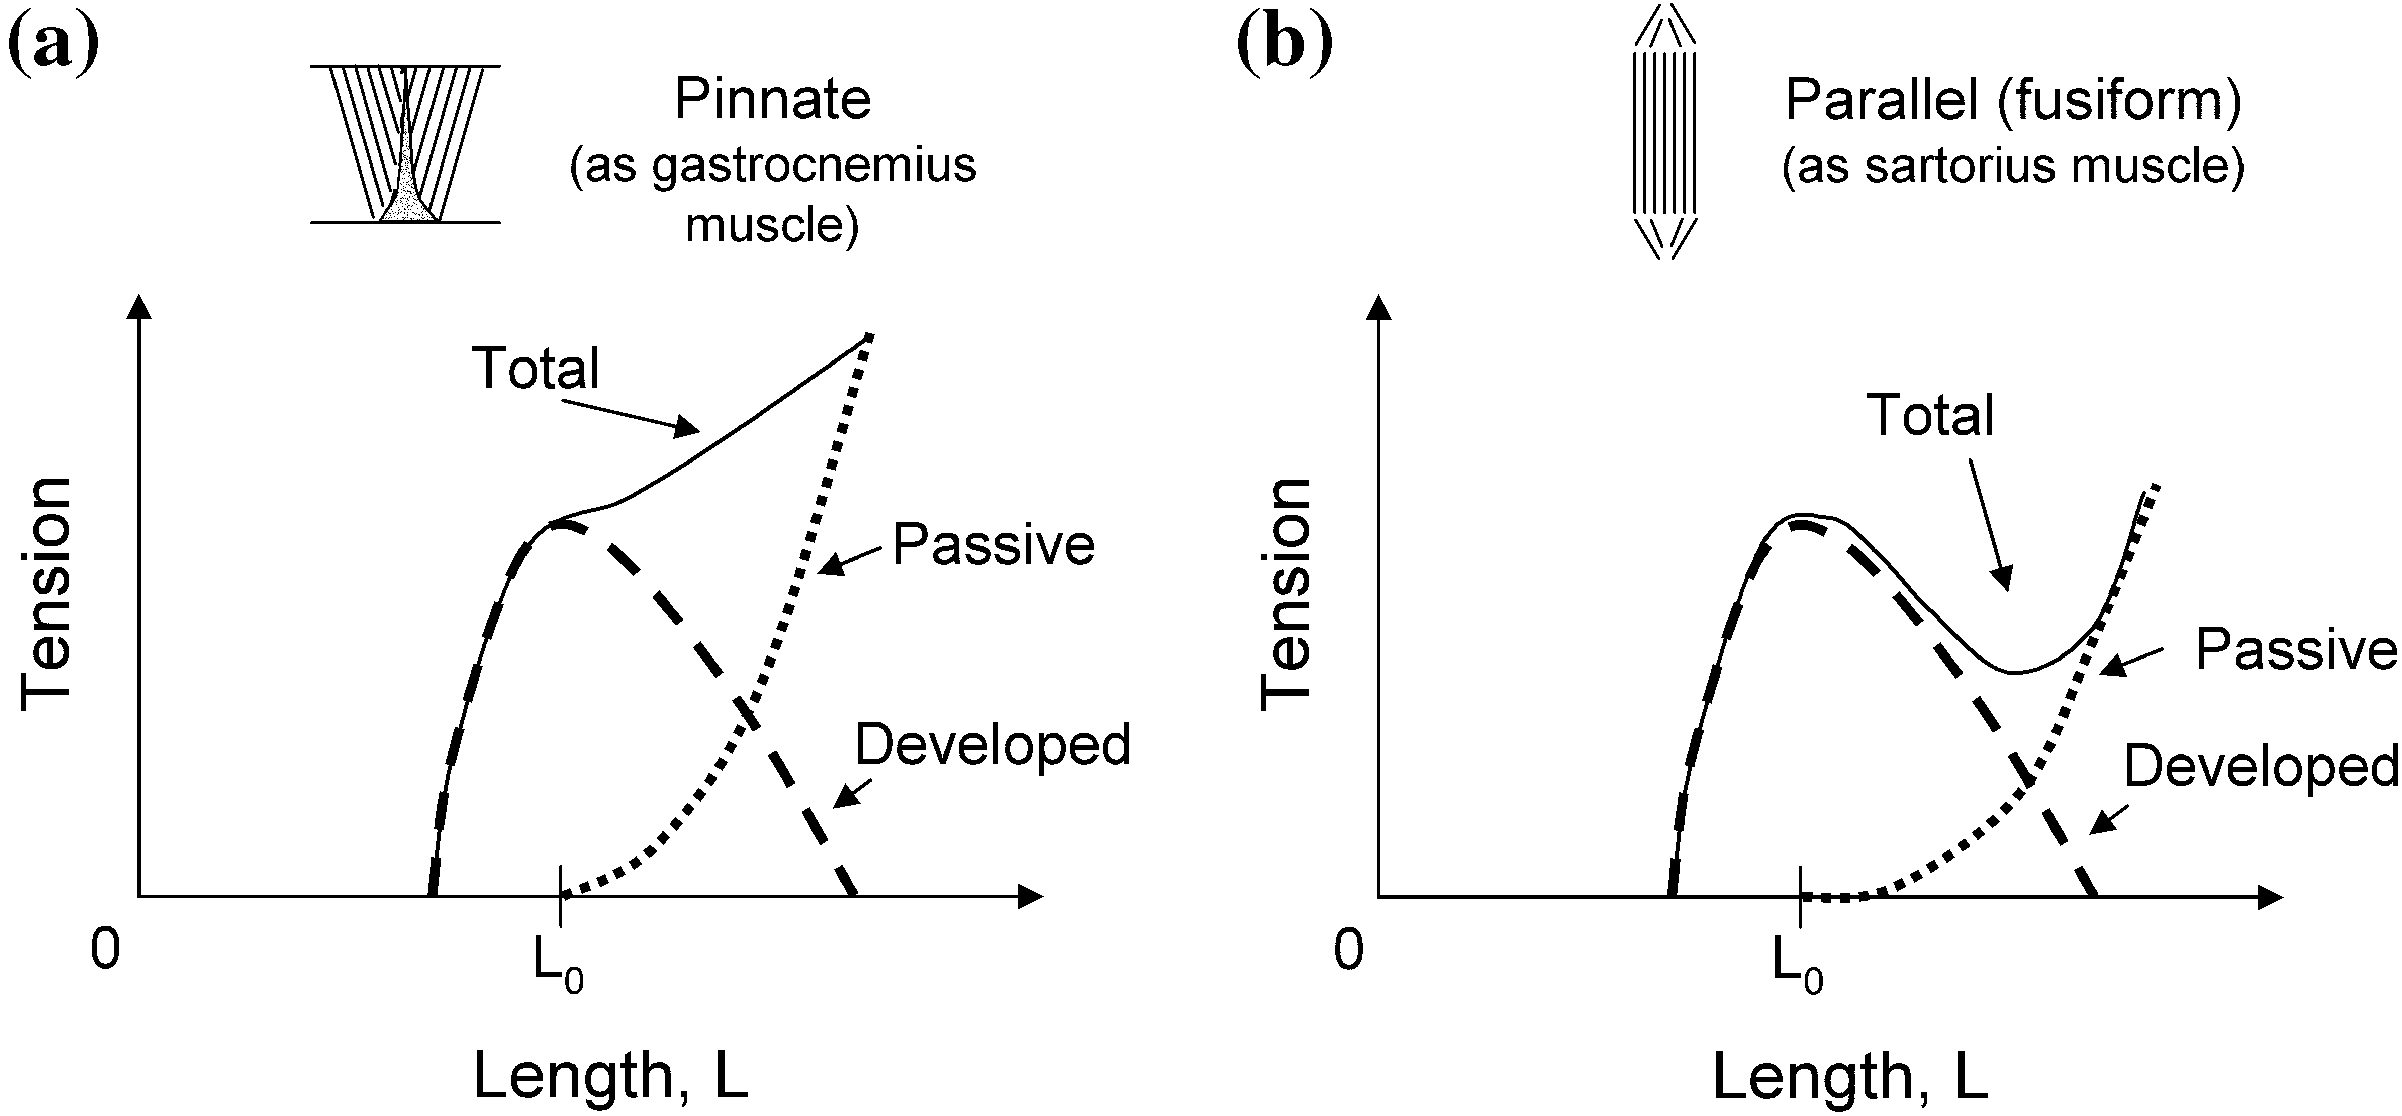
\includegraphics[width=0.8\textwidth]{521.png}
  \caption{Esquema de la tensión pasiva, desarrollada (activa) y total frente a la longitud para músculos pinnados y paralelos. (Basado en \cite{5} y \cite{53}. Ver también \cite{1})}
  \label{fig:521}
\end{figure}



\subsection{Prueba cotidiana del rango limitado de longitud útil del músculo}

La disminución de la tensión que el músculo es capaz de desarrollar cuando es muy corto o largo se puede observar en demostraciones sencillas \cite{4}.

Para la mayoría de nosotros, es difícil hacer dominadas (\textit{pull-ups} o \textit{chin-ups}) o flexiones (\textit{push-ups}) con los brazos completamente extendidos, porque en esta posición inicial los músculos que necesitamos utilizar son mucho más largos que su longitud de reposo. Es mucho más fácil comenzar estos ejercicios a mitad del movimiento, con los músculos más cerca de su longitud de reposo.

Sujeta una pelota (o bolígrafo) con fuerza en un puño cerrado. Pídele a alguien de dimensiones físicas comparables que intente arrebatarte la pelota del puño. Con suerte (y muy probablemente) no podrá. Ahora usa tu otra mano para empujar la parte superior de tu puño cerrado hacia abajo por la muñeca, flexionando la muñeca hacia abajo tanto como sea posible sin infligirte un dolor excesivo. Ahora pídele a tu compañero que intente tomar la pelota. Debería ser una tarea relativamente sencilla. ¿Por qué? Antes de cerrar el puño, los músculos pertinentes suelen estar inicialmente cerca de su longitud de reposo, pero cuando la muñeca está flexionada, los músculos correspondientes son demasiado largos para generar mucha tensión. ¿Cuál es el origen exacto de esto?

Hay 20 músculos en la mano, con una masa total de aproximadamente $91\text{ g}$. La mano completa en sí tiene una masa de unos $600\text{ g}$. Hay 20 músculos en el antebrazo, con una masa de aproximadamente $766\text{ g}$. Nueve de estos, músculos extensores y flexores con una masa combinada de $401\text{ g}$, están conectados a la mano a través de tendones largos (Figs. 5.22 y 5.23). Si estuvieran físicamente en la mano, esta sería sumamente voluminosa.

\begin{figure}[htbp]
  \centering
  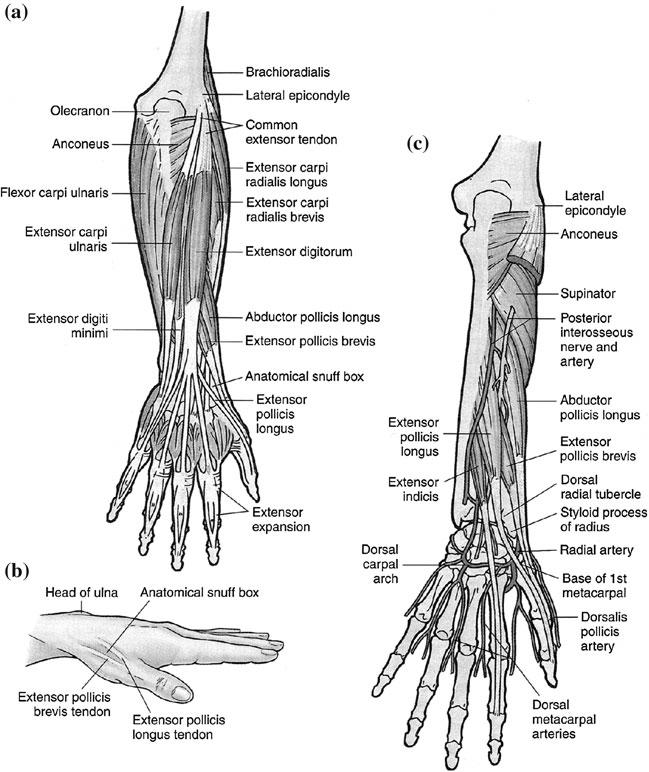
\includegraphics[width=0.55\textwidth]{522.png}
  \caption{Músculos extensores del antebrazo, con \textbf{a} vista posterior de los músculos superficiales, \textbf{b} características seleccionadas de la mano y \textbf{c} músculos más profundos, junto con arterias seleccionadas. También se observan los tendones que se extienden hacia la mano. (De \cite{57}. Utilizado con autorización)}
  \label{fig:522}
\end{figure}

\begin{figure}[htbp]
  \centering
  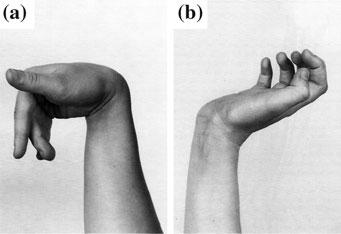
\includegraphics[width=0.7\textwidth]{523.png}
  \caption{Músculos flexores del antebrazo, con vistas anteriores de la primera capa (la más superficial) en \textbf{a}, la segunda capa en \textbf{b}, y la tercera y cuarta capas en \textbf{c}. También se observan los tendones que se extienden hacia la mano. (De \cite{57}. Utilizado con autorización)}
  \label{fig:523}
\end{figure}



Ahora volvamos a sostener la pelota en un puño cerrado. Cuando la muñeca está flexionada (Fig. 5.24a), sin la pelota colocada, los músculos extensores de los dedos ya están estirados, mientras que los flexores de los dedos están flojos (círculos cerrados en la Fig. 5.25a, b). Cuando la muñeca está en esta posición e intentas apretar un objeto, como una pelota, los extensores deben estirarse aún más y los flexores deben aflojarse todavía más (flechas en la Fig. 5.25a, b). Ambos músculos entran en regímenes que superan el rango normal de longitud muscular.

áEste tipo de conocimiento tiene aplicaciones prácticas! Se puede hacer que un asesino con un cuchillo en la mano lo suelte doblando con fuerza su muñeca.

Del mismo modo, no puedes estirar los dedos cuando la muñeca está hiperextendida primero (la mano doblada en la dirección opuesta). Cuando la muñeca está hiperextendida (Fig. 5.24b), sin la pelota colocada, los músculos extensores de los dedos están flojos, mientras que los flexores de los dedos están estirados (círculos cerrados en la Fig. 5.25c, d). Cuando la muñeca está en esta posición e intentas estirar los dedos, los extensores deben aflojarse aún más y los flexores deben estirarse todavía más (flechas en la Fig. 5.25c, d). Nuevamente, ambos músculos entran en regímenes que superan el rango normal de longitud muscular.

\begin{SCfigure}[0.9][htbp]
  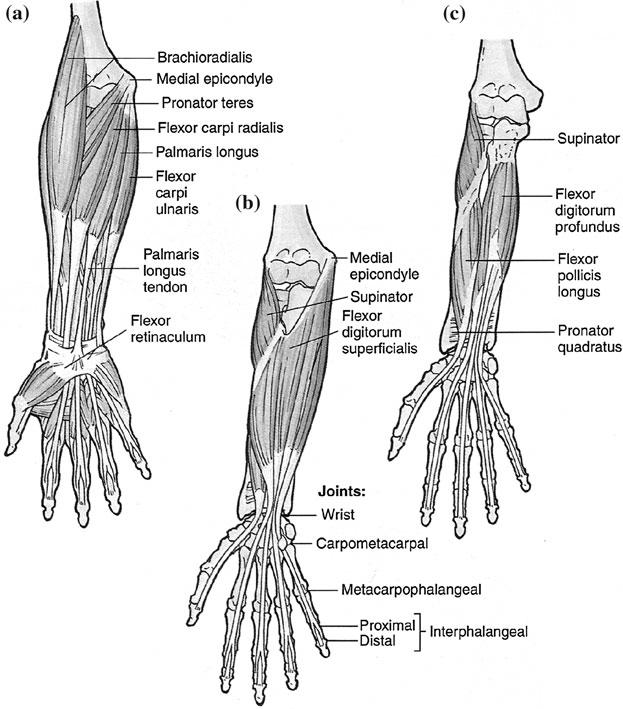
\includegraphics[width=0.5\textwidth]{524.png}
  \caption{Es difícil cerrar el puño con una muñeca fuertemente flexionada \textbf{a} y estirar los dedos con una muñeca fuertemente hiperextendida \textbf{b}. (De \cite{4}. Copyright 1992 Columbia University. Reimpreso con autorización de la editorial)}
  \label{fig:524}
\end{SCfigure}

\begin{SCfigure}[0.8][htbp]
  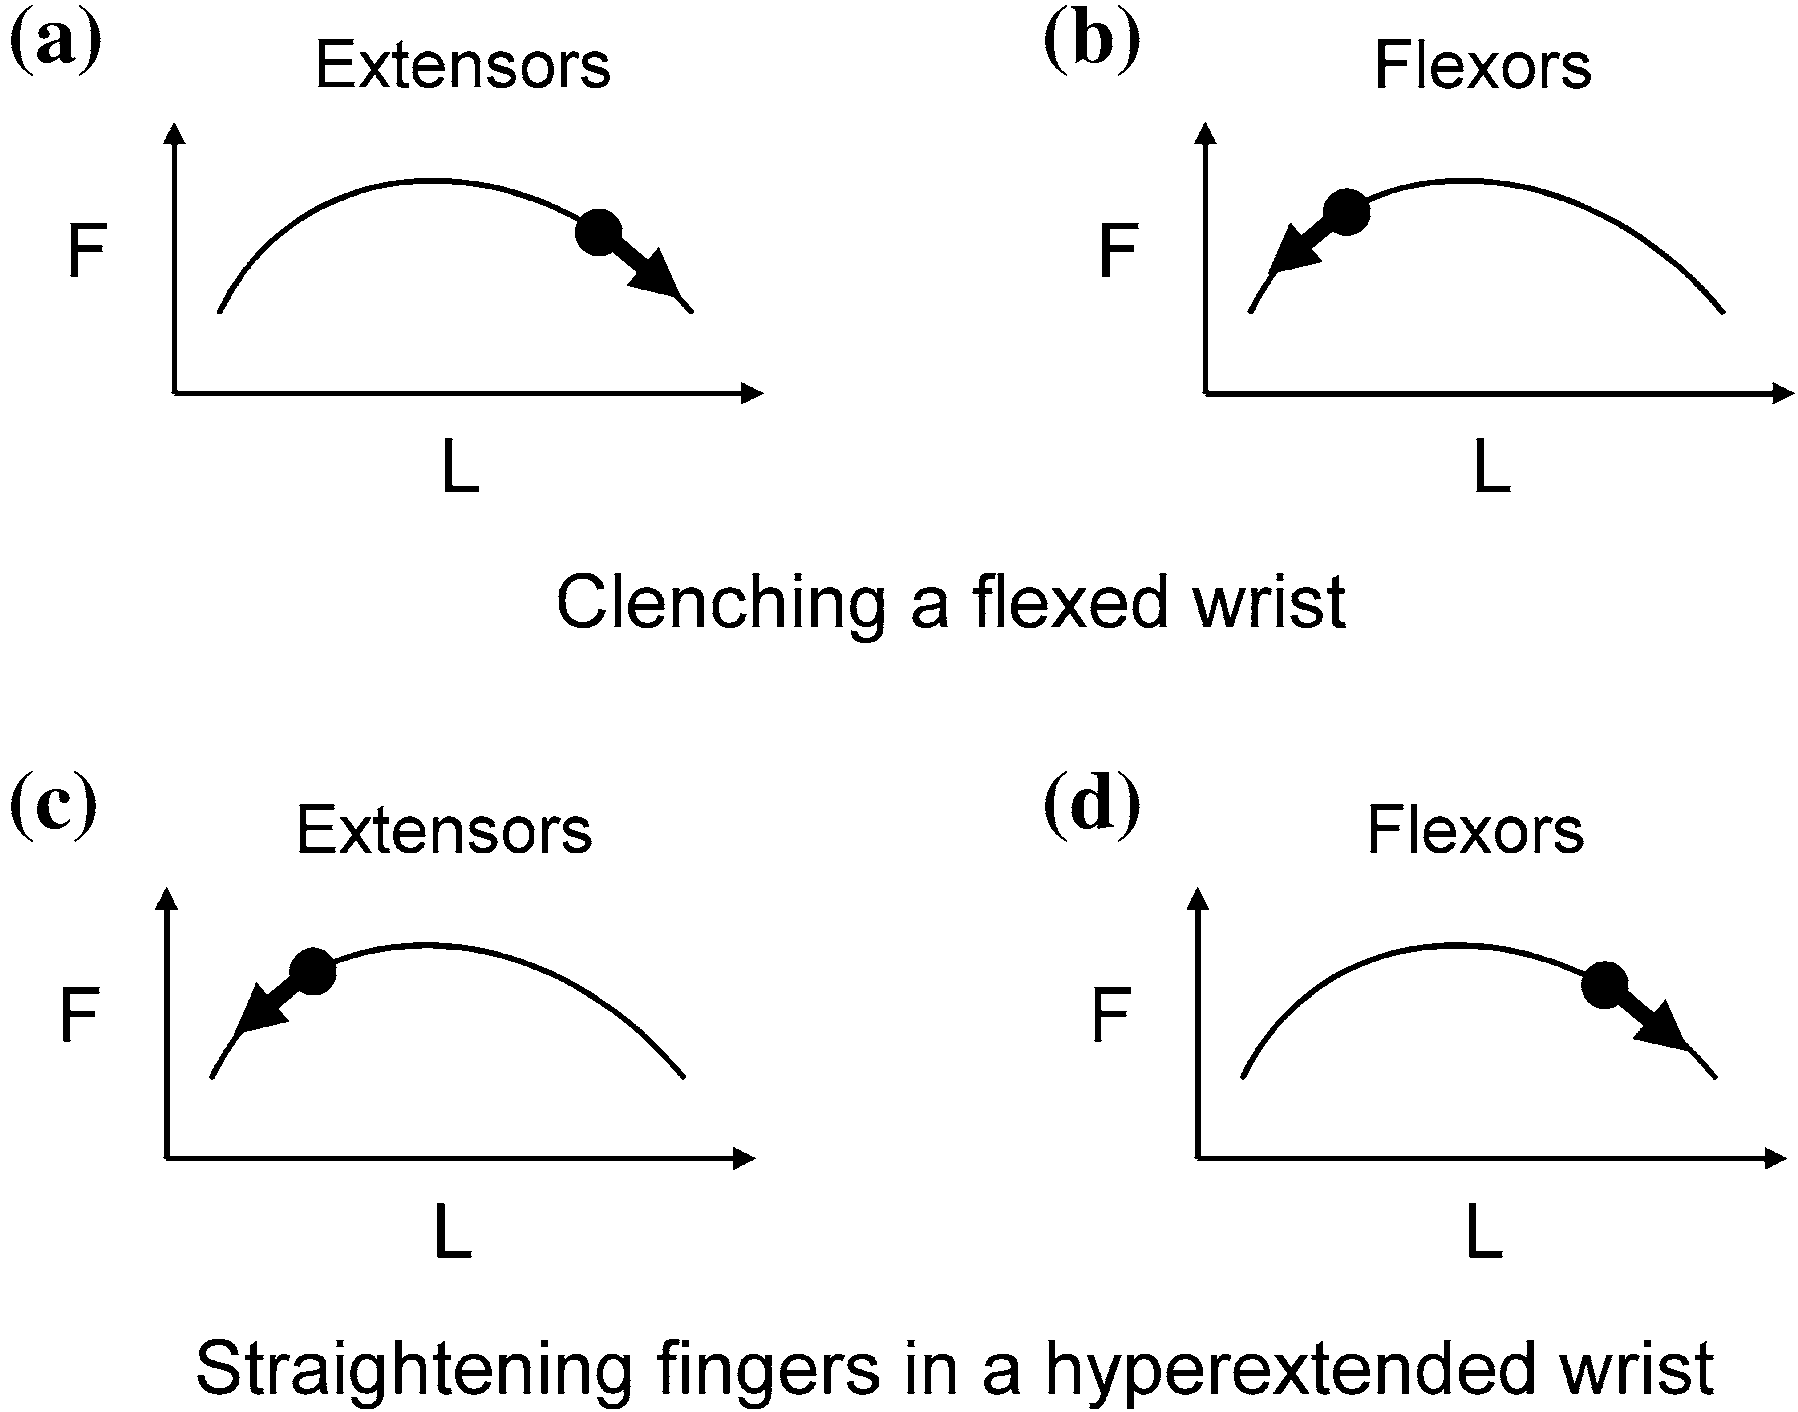
\includegraphics[width=0.55\textwidth]{525.png}
  \caption{Esquema de las fuerzas sobre los extensores y flexores para cerrar el puño con la muñeca flexionada y estirar los dedos con la muñeca hiperextendida, representados por los círculos cerrados. Las flechas muestran el aflojamiento o estiramiento continuo descrito en el texto.}
  \label{fig:525}
\end{SCfigure}



\section{Curva de fuerza-velocidad de Hill}

La tensión máxima $T$ que puede desarrollar un músculo también depende de la rapidez con la que se contrae. Una forma equivalente de decir esto es que la velocidad a la que un músculo puede acortarse depende de cuánta tensión debe generar para vencer una carga, como una masa colgada de su extremo. La velocidad de contracción es $v = -dL/dt = |dL/dt|$, y se mide con el músculo fijo en un extremo y con una carga fija en el otro, es decir, de forma isotónica. (Nuevamente, esta carga fija puede ser una masa de carga suspendida). Se observa experimentalmente que la tensión máxima y la velocidad de contracción siguen la dependencia hiperbólica de la curva de fuerza-velocidad de Hill (Fig. 5.26) \cite{31, 78}, acortándose el músculo más rápidamente con una masa de carga menor. Nótese que los músculos realizan trabajo al contraerse y, como tal, el término tensión se refiere en realidad a la tensión que sienten los objetos unidos a ellos. (Por cierto, Archibald Vivian Hill, quien formuló esta relación de fuerza-velocidad, compartió el Premio Nobel de Fisiología o Medicina en 1922 por su descubrimiento relacionado con la producción de calor en el músculo; gran parte de su trabajo sobre la fuerza generada por los músculos ocurrió después de su investigación galardonada con el Premio Nobel).

\begin{SCfigure}[1.0][htbp]
  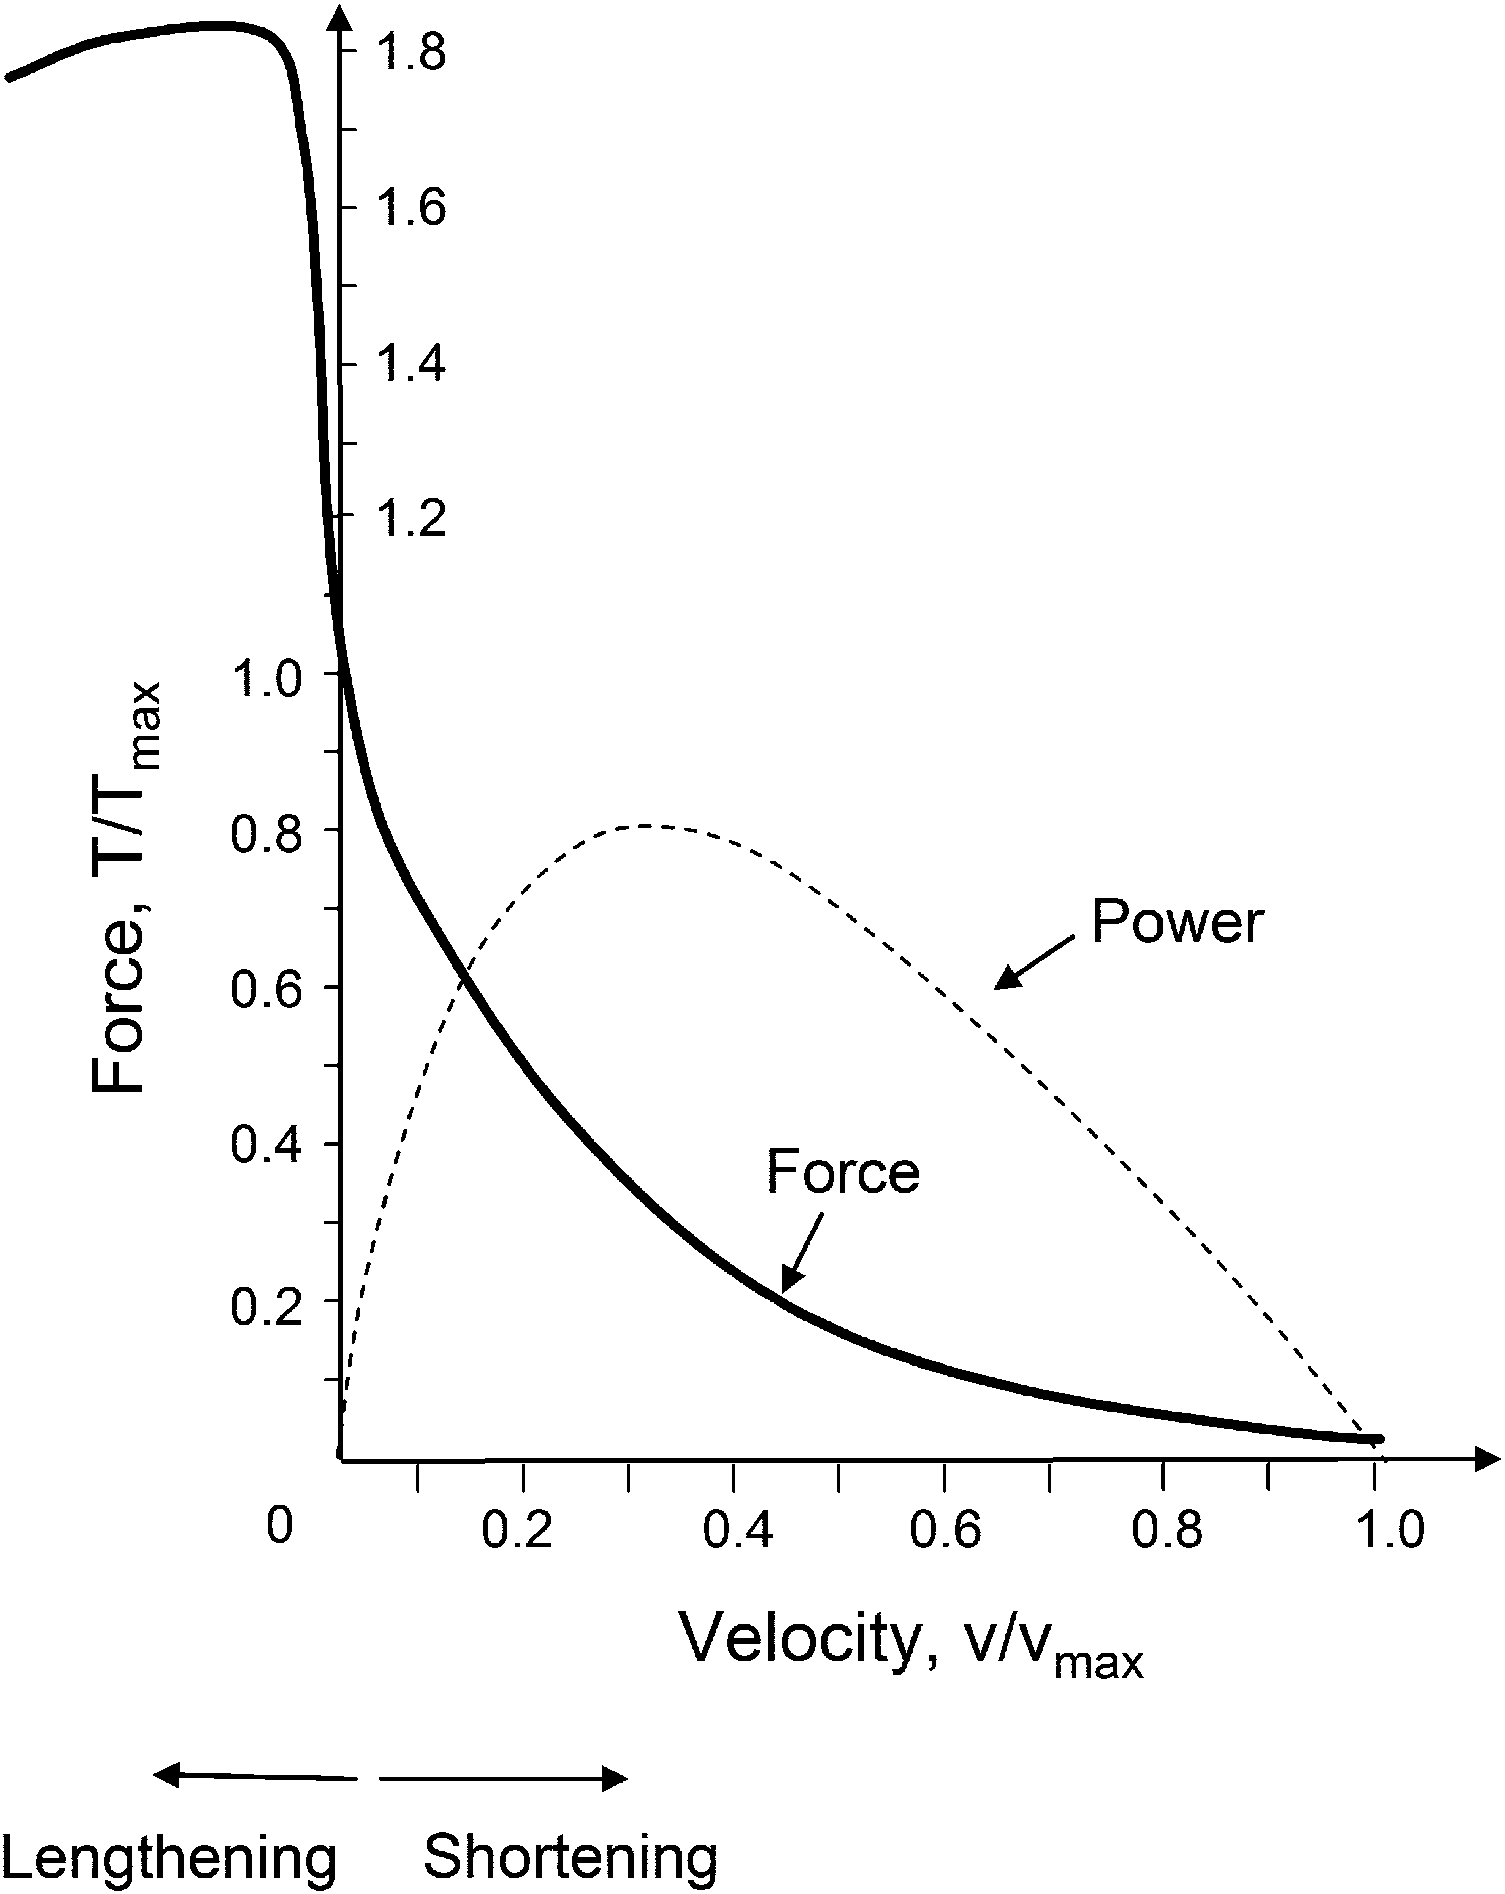
\includegraphics[width=0.45\textwidth]{526.png}
  \caption{Curva de fuerza-velocidad de Hill. Se muestran tanto el acortamiento como el alargamiento del músculo. También se muestra la potencia (Potencia = Fuerza $\times$ velocidad), con unidades verticales arbitrarias. (Basado en \cite{53})}
  \label{fig:526}
\end{SCfigure}



% Control de Calidad: 14 párrafos origen -> 14 párrafos salida. Mapeo 1:1 verificado. Sin omisiones.

La tensión máxima $T_{\text{max}}$ que puede desarrollarse ocurre para $v = 0$ (condiciones isométricas), lo cual es el límite de una contracción muscular muy lenta, $T(v = 0) = T_{\text{max}}$ (a veces llamada $T_0$). $T$ disminuye y se hace cero en $v_{\text{max}}$. Una forma de la curva de fuerza-velocidad de Hill es
\begin{equation}
(T(v) + a)(v + b) = (T_{\text{max}} + a)b
\label{eq:5.20}
\end{equation}
o
\begin{equation}
T(v) = \frac{b T_{\text{max}} - a v}{v + b},
\label{eq:5.21}
\end{equation}
la cual se grafica en la Fig. 5.26. Es válida desde $v = 0$ hasta $v_{\text{max}}$. El lado derecho de (\ref{eq:5.20}) representa el punto en la hipérbola con tensión máxima, con $v = 0$ y $T(v = 0) = T_{\text{max}}$. Podríamos haber elegido los valores en cualquier otro punto de la hipérbola, como aquel con tensión mínima con $v = v_{\text{max}}$ y $T(v = v_{\text{max}}) = 0$, para el cual el lado derecho habría sido $a(v_{\text{max}} + b)$. Claramente estos lados derechos son iguales, por lo que $(T_{\text{max}} + a)b = a(v_{\text{max}} + b)$; esto significa que $v_{\text{max}} = (b/a)T_{\text{max}}$, por lo que solo hay tres parámetros independientes. El tiempo de respuesta efectivo de un músculo de longitud $L$ es $L/v_{\text{max}}$. (¿Por qué?)

Después de reordenar los términos, (\ref{eq:5.21}) se puede expresar como
\begin{equation}
v' = \frac{1 - T'}{1 + T'/k},
\label{eq:5.22}
\end{equation}
donde $v' = v/v_{\text{max}}$, $T' = T/T_{\text{max}}$ y $k = a/T_{\text{max}} = b/v_{\text{max}}$. Típicamente, $0{,}15 < k < 0{,}25$. La Tabla 5.9 proporciona los parámetros de la curva de fuerza-velocidad para varios músculos. Esta curva de fuerza-velocidad de Hill también se puede expresar en términos del torque aplicado a una articulación y la velocidad angular de esa articulación (ver el Problema 5.20).

La curva empírica de fuerza-velocidad de Hill se puede derivar considerando la estadística (más precisamente, la mecánica estadística) de los puentes cruzados en el modelo de filamentos deslizantes. La derivación de este modelo de Huxley se esboza más adelante en este capítulo. Mientras que el modelo de Hill funciona bien en estado estacionario, no lo hace cuando las condiciones del músculo cambian rápidamente (Problema 5.24); el modelo de Huxley funciona bien en ambos casos.

Vimos en (3.87) que la potencia necesaria para mover un objeto es $Fv$, donde $F$ es la fuerza (constante) sobre el objeto y $v$ es la velocidad con la que se mueve. Por lo tanto, la potencia generada por el músculo es
\begin{equation}
P(v) = T(v)v = v \frac{b T_{\text{max}} - a v}{v + b}.
\label{eq:5.23}
\end{equation}
El Problema 5.21 muestra que esto presenta un pico cuando $v \sim 0{,}3 v_{\text{max}}$, para lo cual $T \sim 0{,}3 T_{\text{max}}$. A esta velocidad, la potencia alcanza un valor pico de $\sim 0{,}1 T_{\text{max}} v_{\text{max}}$ (Fig. 5.26). Las bicicletas tienen cambios (engranajes) que aprovechan esto, manteniendo la velocidad de acortamiento muscular cerca del valor en el que se logra este pico de potencia. Esto es análogo a cambiar de marcha en los automóviles que viajan a diferentes velocidades para que sus motores puedan funcionar a unas rpm cercanas al torque máximo.

\begin{table}[htbp]
\centering
\caption{Parámetros para la relación de fuerza-velocidad de Hill en músculos sin piel (skinned), con las fuerzas normalizadas por unidad de área.}
\label{tab:59}
\small
\begin{tabularx}{\textwidth}{X >{\centering\arraybackslash}X >{\centering\arraybackslash}X >{\centering\arraybackslash}X}
\toprule
\textbf{Músculo} & \textbf{Fuerza isométrica, $T_{\text{max}}$ (MPa)} & \textbf{Velocidad máxima, $v_{\text{max}}$ (FL/s)$^a$} & \textbf{$a/T_{\text{max}}$} \\
\midrule
Sóleo humano ($15\text{ }^\circ\text{C}$)$^b$ & $0{,}145$ & $0{,}52$ & $0{,}037$ \\
Gastrocnemio humano ($15\text{ }^\circ\text{C}$)$^b$ & $0{,}136$ & $0{,}64$ & $0{,}034$ \\
Sóleo de mono ($15\text{ }^\circ\text{C}$)$^b$ & $0{,}146$ & $0{,}7$ & $0{,}044$ \\
Gastrocnemio de mono ($15\text{ }^\circ\text{C}$)$^b$ & $0{,}160$ & $0{,}69$ & $0{,}040$ \\
Psoas de conejo ($20\text{ }^\circ\text{C}$)$^c$ & $0{,}246$ & $3{,}26$ & $0{,}10$ \\
Sóleo de rata ($20\text{ }^\circ\text{C}$)$^c$ & $0{,}234$ & $1{,}94$ & $0{,}05$ \\
\bottomrule
\end{tabularx}
\begin{flushleft}
    \small $^a$FL es la longitud de la fibra (\textit{fiber length}). \\
    $^b$\cite{77} \\
    $^c$\cite{75} \\
    Utilizando datos de \cite{51}.
\end{flushleft}
\end{table}

La curva de fuerza-velocidad de Hill en realidad se refiere únicamente al elemento contráctil del músculo. Podemos relacionar la tensión a través de todo el músculo o fibra muscular, $T$, con su longitud, $L$, utilizando el modelo de dos elementos de Hill para un músculo esquelético \cite{40, 41}. Este consiste en el elemento contráctil descrito por la curva de fuerza-velocidad de Hill en serie con un elemento elástico; este es el modelo mostrado en la Fig. 5.15 sin el amortiguador. La tensión $T$ es la misma a través de todo el músculo, el elemento contráctil y el resorte. La longitud del músculo es la suma de las longitudes del elemento contráctil y del resorte, $L = x_{\text{T1}} + x_{\text{T2}} = x_{\text{E1}} + x_1 + x_{\text{E2}} + x_2$ (usando la notación de la discusión de la Fig. 5.15), y por lo tanto $dL/dt = dx_1/dt + dx_2/dt$. La velocidad de contracción del elemento contráctil es $v = -dx_{\text{T1}}/dt = -dx_1/dt$, por lo que $dx_2/dt = dL/dt - dx_1/dt = dL/dt + v$.

Utilizando (\ref{eq:5.20}), esta velocidad es $v = b(T_{\text{max}} - T)/(T + a)$. La tasa de cambio temporal de la tensión se puede determinar utilizando la regla de la cadena, $dT/dt = (dT/dx_2)(dx_2/dt)$. Con $dT/dx_2 = k$, la constante del resorte, la tensión a través de todo el músculo $T$ se relaciona con su longitud $L$ mediante
\begin{equation}
\frac{dT}{dt} = k \left[ \frac{dL}{dt} + \frac{b(T_{\text{max}} - T)}{T + a} \right].
\label{eq:5.24}
\end{equation}
Esta ecuación solo se puede utilizar si $T_{\text{max}}$ no cambia (o no cambia mucho) durante el acortamiento muscular a velocidad constante, como en el caso de pequeñas contracciones cerca del pico de la curva de tensión-longitud (Fig. 5.19).

A niveles más bajos de excitación muscular, hay una menor fuerza contráctil a cada velocidad, como se ve en la Fig. 5.27. Además, los músculos por lo general no mantienen una velocidad cero, como se supone en la Fig. 5.19, o una longitud constante, como se supone en la Fig. 5.26. La respuesta de un músculo depende realmente tanto de su longitud como de la velocidad de contracción, como se representa en la Fig. 5.28. Esto muestra que cuando la longitud del músculo no es $L_0$, la velocidad máxima de contracción es menor que $v_{\text{max}}$.

\begin{SCfigure}[0.8][htbp]
  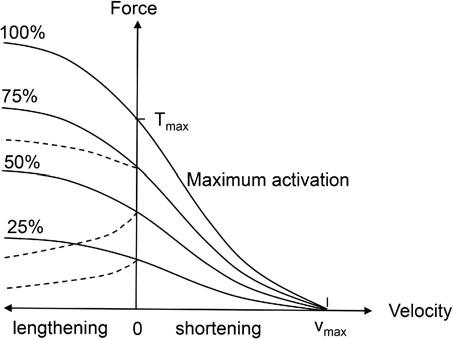
\includegraphics[width=0.55\textwidth]{527.png}
  \caption{Curvas de fuerza-velocidad a diferentes niveles de activación muscular, para una longitud de músculo dada. Todas las curvas de acortamiento siguen las curvas de fuerza-velocidad de Hill, pero para el alargamiento las curvas son diferentes para la actividad isotónica (curvas continuas) y la actividad de isovelocidad (curvas discontinuas). (Basado en \cite{81})}
  \label{fig:527}
\end{SCfigure}



Los modelos simples de movimiento comúnmente asumen que la fuerza muscular depende de la longitud del músculo (y no de la velocidad de contracción, la cual implícitamente se asume que es lenta) o de la velocidad de contracción (y no de la longitud del músculo, la cual implícitamente se asume que permanece cerca de la correspondiente a la fuerza muscular máxima), pero no de ambas (como en la Fig. 5.28). Esto se hace bien porque es más simple de esa manera o porque las condiciones específicas realmente lo justifican. (Ver los Problemas 5.25 y 5.26). Utilizamos estas suposiciones alternativas en el Cap. 3 para modelar el lanzamiento y el salto.

\begin{figure}[htbp]
  \centering
  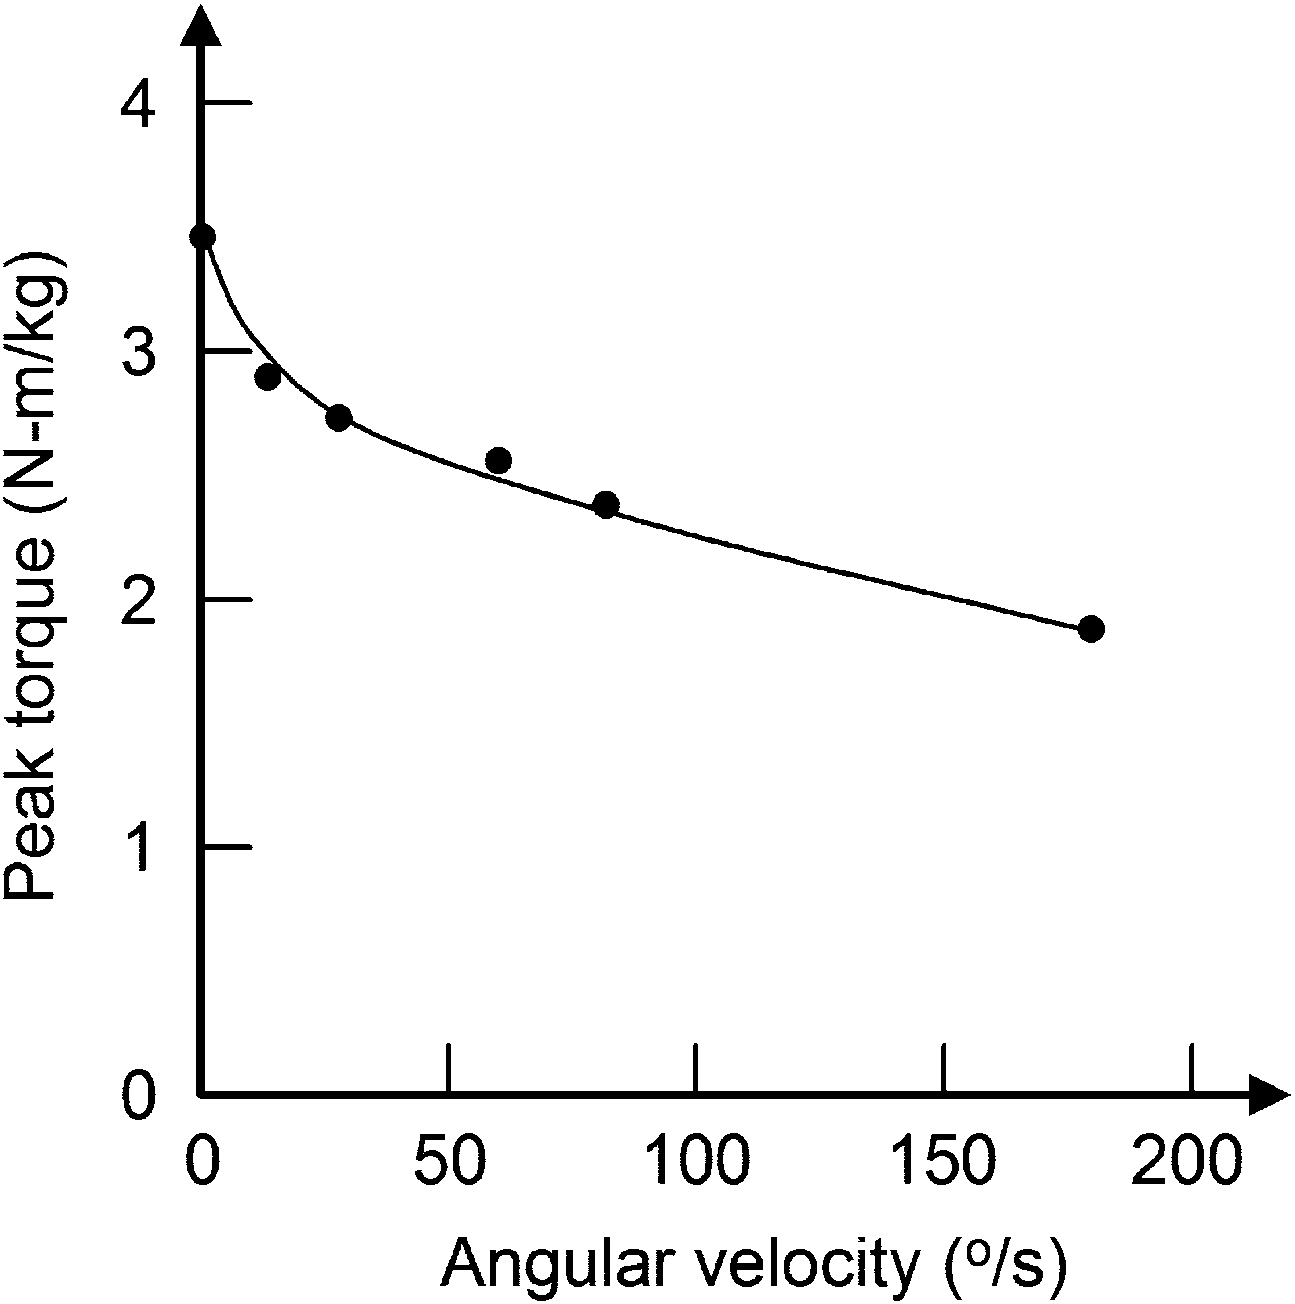
\includegraphics[width=0.55\textwidth]{528.png}
  \caption{Gráfico tridimensional que muestra la tensión de la parte activa de un músculo frente a la velocidad y la longitud. Esto es para la activación máxima del músculo y excluye la respuesta pasiva del músculo. (Basado en \cite{81})}
  \label{fig:528}
\end{figure}



Hasta ahora hemos considerado el acortamiento muscular desde velocidades de $0$ a $v_{\text{max}}$. Esto es importante para realizar trabajo positivo. Sin embargo, se observa que la Fig. 5.26 se extiende a la izquierda de $v = 0$, donde hay alargamiento muscular ($dL/dt > 0$). La tensión que se desarrolla en este régimen de contracción excéntrica es de aproximadamente $1{,}8 T_{\text{max}}$. En este régimen, el músculo se utiliza para el frenado, no para realizar trabajo positivo. Esta aplicación se utiliza para frenar el movimiento (excéntrico), resistir la tracción, actividades isométricas (longitud muscular constante) y mantener el cuerpo estable, como al estar de pie. Recuerde que se pierden $100\text{ J}$ en cada paso al correr. Casi la mitad de esta energía es absorbida por la acción de frenado de los músculos de las piernas. Cuando los músculos no están completamente activados, esta tensión tan grande en el frenado siempre ocurre para movimientos isotónicos, pero no siempre para modos de isovelocidad, como se observa en la Fig. 5.27.

La Figura 5.29 muestra datos experimentales del torque que se puede desarrollar en la extensión de la rodilla frente a la velocidad del cambio angular \cite{21}. En esta figura, las fuerzas generadas son proporcionales a este torque, y la velocidad de cambio de la longitud muscular es proporcional a esta velocidad de cambio angular. Esto es análogo a interrelacionar la fuerza muscular frente a la longitud con el torque de la rodilla frente al ángulo. (Ver el Problema 5.20). La Figura 5.12 muestra que la velocidad angular máxima y el torque dependen de la fracción de fibras FT.

\begin{SCfigure}[0.8][htbp]
  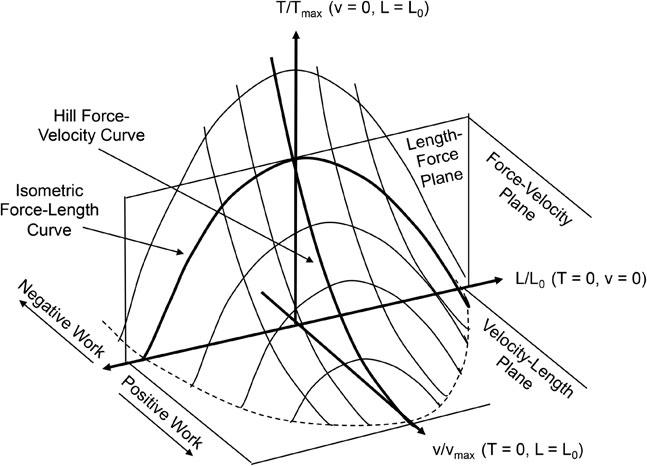
\includegraphics[width=0.55\textwidth]{529.png}
  \caption{Torque (por unidad de masa corporal) frente a la velocidad angular de la rodilla para la extensión de la rodilla. (Basado en \cite{21} y \cite{73})}
  \label{fig:529}
\end{SCfigure}



% Control de Calidad: 10 párrafos origen -> 10 párrafos salida. Mapeo 1:1 verificado. Sin omisiones.

En el levantamiento de pesas, se puede levantar una carga más pesada si se sube rápidamente, es decir, si se realiza un ``envión'' o ``tirón'' (\textit{jerked}), que si se mueve de forma más lenta y fluida. Esto no es realmente contradictorio con la curva de fuerza-velocidad de Hill porque el levantador está aprovechando las mayores fuerzas musculares que son posibles antes de que los filamentos puedan ganar velocidad. Por lo tanto, se pueden levantar pesos más grandes mediante un levantamiento rápido hasta la altura de los hombros y luego un envión hasta la extensión vertical completa ---el ``envión'' o ``dos tiempos'' (\textit{clean-and-jerk})--- que mediante un levantamiento rápido hasta la altura de los hombros y luego un levantamiento lento hasta la extensión vertical completa ---la ``fuerza'' (\textit{press}). (Por cierto, la fuerza ya no es un evento competitivo porque es difícil de distinguir del envión). Un tercer movimiento de levantamiento de pesas es la ``arrancada'' o ``arranque'' (\textit{snatch}), en el cual el peso se levanta en un solo movimiento continuo. Los récords mundiales para la arrancada y el envión son de $151{,}0\text{ kg}$ y $190{,}0\text{ kg}$, respectivamente, para mujeres ($m_{\text{b}} \ge 75\text{ kg}$, a partir de 2014) y de $214{,}0\text{ kg}$ y $263{,}5\text{ kg}$ para hombres ($m_{\text{b}} \ge 105\text{ kg}$). (Para más información sobre esto, ver el Problema 5.7).

\section{El sistema combinado músculo-tendón}

La fuerza desarrollada, la longitud total y la velocidad de contracción del músculo en sí y las del sistema combinado músculo-tendón pueden ser muy diferentes. Acabamos de examinar las propiedades de los músculos y examinamos las de los tendones en el capítulo anterior, y ahora analizaremos el sistema combinado porque esto es lo que realmente importa. Además, en procedimientos quirúrgicos que involucran trasplantes de tendones, comprender y medir las propiedades pasivas y activas de los sistemas combinados de músculo-tendón puede ser muy útil \cite{47, 48}; esto es muy similar a la necesidad de compatibilidad de las propiedades mecánicas al evaluar la idoneidad de los implantes biomédicos que vimos en el Cap. 4.

En el sistema combinado, la fuerza se puede sostener cuando la longitud de la fibra muscular excede $\sim 0{,}7 L_0$, donde $L_0$ es (aún) la longitud óptima de la fibra muscular, y esto ocurre cuando la longitud del sistema total de músculo + tendón excede $L_{\text{T,s}} + 0{,}7 L_0$, donde $L_{\text{T,s}}$ es la longitud libre o relajada del tendón \cite{82}. (Esto es válido para músculos fusiformes y paralelos, y este y otros parámetros que definiremos deben ser modificados para músculos pinnados).

La relación $L_{\text{T,s}}/L_0$ es un parámetro importante para describir el efecto combinado del músculo y el tendón. Cuando esta es grande, digamos $\sim 10$, el sistema general es muy flexible (o complaciente) y el tendón afecta con gran fuerza a las curvas generales de fuerza frente a longitud, y cuando es pequeña, $\sim 1$, el sistema general se considera rígido y el efecto del tendón es relativamente pequeño. En los seres humanos, esta relación es de $\sim 11$ para el sóleo, $\sim 9$ para el gastrocnemio y $\sim 7$ para otros músculos plantarflexores; de $\sim 3$ para los vastos y $\sim 5$ para el recto femoral en el cuádriceps; de $\sim 2$ para el semitendinoso y $\sim 7$ para el semimembranoso/bíceps (largo) en los isquiotibiales; y de $\sim 0{,}2$ para los músculos uniarticulares de la cadera \cite{82}.

La Figura 5.30 muestra cómo cambia la respuesta del músculo solo (incluidas sus partes activa y pasiva, como en la Fig. 5.21) cuando se incluye el tendón. Lo que se grafica es la longitud total menos la del tendón libre, por lo que es realmente la longitud del músculo más el cambio en la longitud del tendón. Para el tendón muy rígido representado en \textbf{a}, la curva se estira lateralmente solo un poco y el cambio en la región ascendente ($L < L_0$), donde la respuesta pasiva del músculo es pequeña, cambia solo un poco. Para el tendón muy flexible (o complaciente) en \textbf{b}, la respuesta es muy diferente, como se observa en los cambios muy grandes en la región ascendente. Esto está muy distorsionado en comparación con la respuesta del músculo solo, siendo la longitud de la parte ascendente de la curva mucho mayor, y ocurriendo el máximo del músculo desarrollado más cerca de $1{,}5 L_0$ que de $L_0$; en el pico de fuerza desarrollada, los tendones se estiran una fracción considerable de la longitud óptima del músculo.

\begin{figure}[htbp]
  \centering
  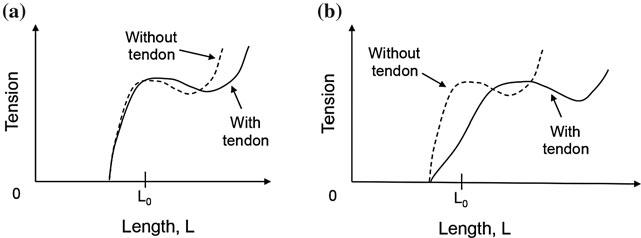
\includegraphics[width=0.8\textwidth]{530.png}
  \caption{Fuerza frente a la longitud para un músculo y tendón combinados, que incluye la respuesta máxima activada y la respuesta pasiva de los músculos para tendones que son o bien \textbf{a} muy rígidos ($L_{\text{T,s}}/L_0 = 3$) o bien \textbf{b} muy flexibles (o complacientes) $L_{\text{T,s}}/L_0 = 15$ para condiciones isométricas. (Basado en \cite{82})}
  \label{fig:530}
\end{figure}



Hasta ahora hemos considerado condiciones isométricas. La longitud relativa de los tendones con respecto al músculo también afecta la velocidad de contracción y la dinámica del sistema total. Para valores muy grandes de $L_{\text{T,s}}/L_0$, como ocurre con el sóleo, los factores limitantes de la tasa de generación de fuerza son la dinámica del sistema músculo-tendón; para relaciones muy pequeñas, como en el caso de los músculos uniarticulares de la cadera, la activación del músculo es el factor limitante de la tasa; y para relaciones intermedias, como para el recto femoral, ambos procesos son importantes \cite{82}.

\section{El modelo de filamentos deslizantes: perspectiva nanoscópica}

El cuerpo tiene varias proteínas motoras que inducen el movimiento dirigido. La miosina (Figs. 5.7, 5.18, 5.19 y 5.31) realiza esto en los músculos \cite{62}. La cinesina (\textit{kai-nee'sin}) y la dineína (\textit{die-nee-in}) dirigen el transporte sobre microtúbulos en el cuerpo (Fig. 5.32) \cite{6, 10, 11, 24, 27, 42, 69, 74}. (Ambas se utilizan en el transporte a larga distancia en el cuerpo. Dentro de la célula, la cinesina se utiliza para el transporte desde el centro de la célula hacia su periferia, mientras que la dineína se utiliza para el transporte desde la periferia celular hacia su centro). Dicho transporte dirigido es preferible a la difusión porque proporciona un movimiento direccionado y un movimiento que es más rápido que la difusión. Como se describe con más detalle en el Cap. 7, en una dimensión la difusión conduce a una propagación lenta, de tipo gaussiana y no dirigida de la especie sobre una distancia $x \sim \sqrt{2 D_{\text{diff}} t}$ en un tiempo $t$, donde $D_{\text{diff}}$ es el coeficiente de difusión. El movimiento dirigido es necesario para el movimiento muscular. La Figura 5.31 muestra la cabeza de una molécula de miosina de un filamento grueso unida a una molécula de actina etiquetada como $x$ en un filamento delgado (Fig. 5.31a). Este acoplamiento único es un puente cruzado. Esta etapa de la interacción se denomina la posición armada o de reposo (\textit{cocked position}). El ATP se hidroliza para formar ADP + fosfato inorgánico + energía (ver el Cap. 6) y esta energía se utiliza para contorsionar la molécula de miosina, que todavía está unida a la misma molécula de actina, hacia una nueva configuración. Este movimiento, junto con la acción simultánea de otros puentes cruzados en los mismos filamentos, hace que el filamento delgado se deslice hacia la izquierda. Esta es la etapa de golpe de fuerza o carrera de potencia (\textit{power stroke}). La molécula de miosina se desprende (la fase de desprendimiento), se relaja y luego se une a la molécula de actina adyacente etiquetada como $x + 1$ (Fig. 5.31d) en el filamento delgado (la fase de unión). ¿Cuántos puentes cruzados hay en un músculo? ¿Cuánta fuerza se genera por puente cruzado? Necesitamos conectar esta perspectiva nanoscópica de los puentes cruzados con la observación macroscópica de que los músculos generan hasta $\sim 30\text{ N/cm}^2$.

\begin{figure}[htbp]
  \centering
  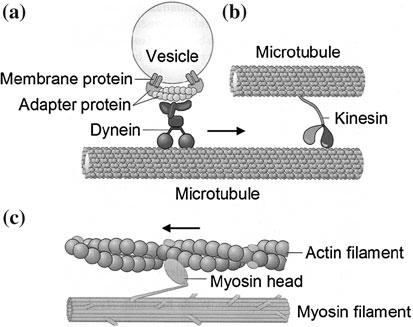
\includegraphics[width=0.7\textwidth]{531.png}
  \caption{Deslizamiento de los miofilamentos, con \textbf{a} unión de la cabeza de miosina a un sitio activo de actina (sitio $x$), \textbf{b} el golpe de fuerza (carrera de potencia) en el cual la cabeza de miosina hidroliza ATP, se deforma y mueve el filamento delgado, \textbf{c} la cabeza de miosina se desprende y se relaja, y \textbf{d} la cabeza de miosina se vuelve a unir a un nuevo sitio de actina ($x + 1$) para un nuevo ciclo. (Basado en \cite{67} y \cite{71})}
  \label{fig:531}
\end{figure}

\begin{SCfigure}[0.9][htbp]
  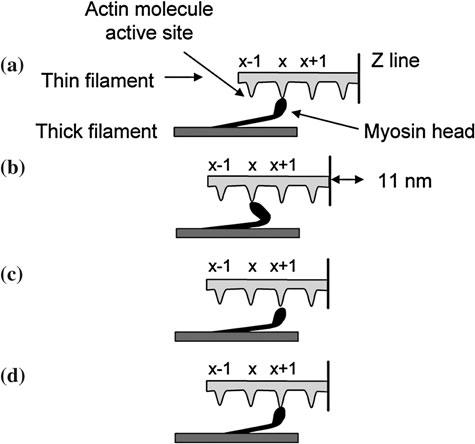
\includegraphics[width=0.5\textwidth]{532.png}
  \caption{Comparación de proteínas motoras, con \textbf{a} transporte de una vesícula a lo largo de una vía de microtúbulo por dineína, \textbf{b} transporte de un microtúbulo sobre una vía de microtúbulo por cinesina, y \textbf{c} movimiento del filamento de actina por un filamento de miosina. (De \cite{68})}
  \label{fig:532}
\end{SCfigure}



Cada músculo tiene entre $10^4$ y $10^6$ fibras. Cada fibra tiene un diámetro de $10\text{--}80\ \mu\text{m}$. Supongamos que $50\ \mu\text{m}$ es un valor típico, de modo que hay $\sim 1/(50\ \mu\text{m})^2 = 4 \times 10^4\text{ fibras/cm}^2$. Cada fibra tiene desde varios cientos hasta varios miles de miofibrillas, y supongamos que hay $2000$ de ellas. Cada miofibrilla tiene unos $1500$ filamentos gruesos de miosina y $3000$ filamentos delgados de actina, y de $\sim 1 \times 10^4$ a $1{,}7 \times 10^5$ sarcómeros. Estos filamentos están dispuestos de manera ordenada como en la Fig. 5.6a, b (inferior). Cada filamento grueso tiene $200$ moléculas de miosina.

En un sarcómero dado, todos los puentes cruzados están en paralelo, por lo que las fuerzas de cada uno se suman para cada filamento. Esto es análogo a muchas personas que tiran de una cuerda en un juego de tracción (tira y afloja) o que reman juntas en una embarcación o galera, donde sus fuerzas combinadas se suman. Todos los filamentos en un sarcómero (miofibrilla) se suman en paralelo, por lo que estas fuerzas se suman. Todas las miofibrillas en una fibra se suman en paralelo, de modo que sus fuerzas se suman. Todas las fibras musculares se suman en paralelo, por lo que sus fuerzas se suman.

Por lo tanto, dentro del ancho de un medio sarcómero hay:
\begin{align*}
& (4 \times 10^4\text{ fibras/cm}^2) \times (2000\text{ miofibrillas/fibra}) \\
& \quad \times (1500\text{ filamentos gruesos/miofibrilla}) \times (200\text{ moléculas de miosina/filamento grueso}) \\
& \quad \simeq 1 \times 10^{13}\text{ moléculas de miosina/cm}^2.
\end{align*}
Esto significa que la fuerza desarrollada a través de cada puente cruzado es
\begin{equation}
\sim \frac{30\text{ N/cm}^2}{1 \times 10^{13}\text{ moléculas de miosina/cm}^2} \sim 3 \times 10^{-12}\text{ N} = 3\text{ pN}.
\label{eq:5.25}
\end{equation}
Esta es también una conclusión del modelo de filamentos deslizantes de Huxley para la curva de fuerza-velocidad de Hill. La medición directa de la interacción de un solo puente cruzado de actina-miosina mediante pinzas ópticas (las cuales son trampas láser enfocadas que se utilizan para confinar estas moléculas) ha demostrado que se generan de $3\text{--}4\text{ pN}$ por puente cruzado, y la distancia del golpe de fuerza (Fig. 5.31b) ---el movimiento relativo de los filamentos por cada hidrólisis de ATP--- es de $11\text{ nm}$ (Fig. 5.33). Esta es verdaderamente una perspectiva nanoscópica de los músculos. (En el Problema 5.30 usted puede calcular el trabajo realizado por este movimiento y caracterizarlo en términos de la fracción de la energía liberada en la hidrólisis del ATP, la cual se describe en el próximo capítulo).

\begin{SCfigure}[0.9][htbp]
  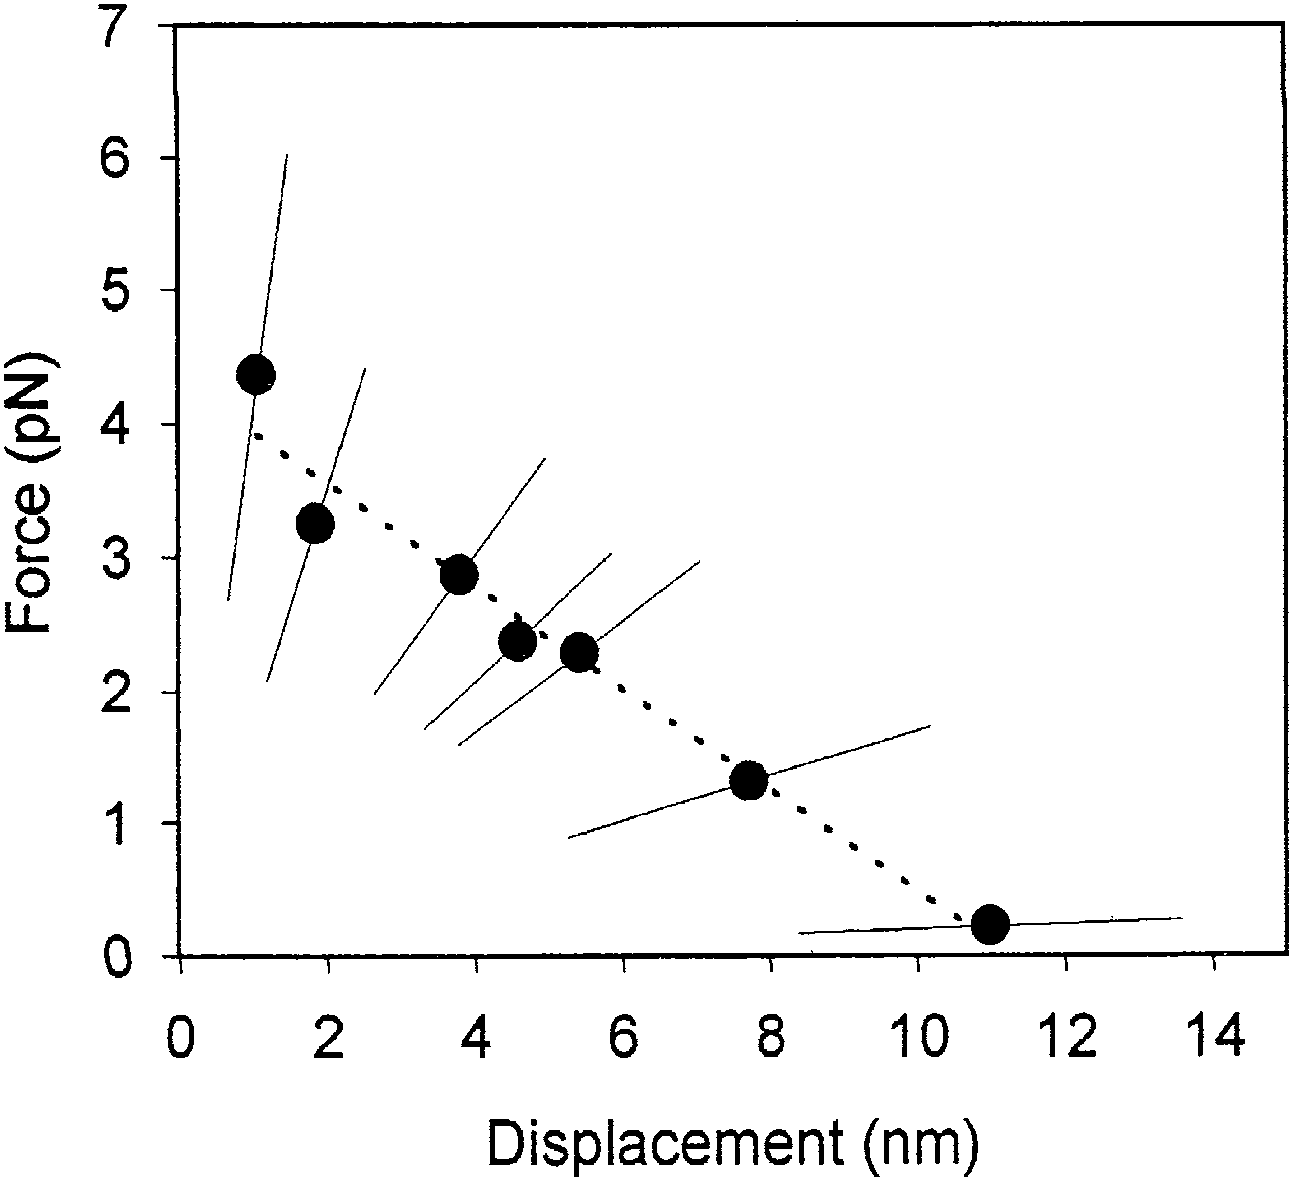
\includegraphics[width=0.5\textwidth]{533.png}
  \caption{Curva de fuerza frente a desplazamiento de una sola molécula de miosina interactuando con una molécula de actina durante un golpe de fuerza (carrera de potencia), según mediciones con ``pinzas ópticas''. (De \cite{17}. Utilizado con autorización de la Biophysical Society)}
  \label{fig:533}
\end{SCfigure}



Al examinar el efecto de los puentes cruzados en los sarcómeros para ejercer fuerzas, consideramos únicamente los puentes cruzados en los sarcómeros de una sección transversal del músculo. Estos se suman para dar la fuerza por área total para el músculo. Sin embargo, hay $\sim 1 \times 10^4\text{--}1{,}7 \times 10^5$ sarcómeros a lo largo de la longitud de cada fibra en el músculo. Estas decenas de miles de sarcómeros no aumentan la fuerza ejercida por el músculo, sino que cumplen una función bastante importante, aunque muy diferente. La cantidad necesaria de rotación alrededor de las articulaciones solo puede ocurrir si hay un cambio suficiente en la longitud del músculo (o en la longitud combinada de tendón más músculo). Debido a que el cambio efectivo en la longitud del sarcómero y del músculo es de solo aproximadamente $\pm 30\%$, el cambio en la longitud total está controlado por la longitud del músculo en reposo, la cual depende del número de sarcómeros a lo largo de la longitud de las fibras. (Esto se relaciona con la segunda ventaja del diseño pinnado de los músculos).

% Control de Calidad: 11 párrafos origen -> 11 párrafos salida. Mapeo 1:1 verificado. Sin omisiones.

Nuestro modelo de puente cruzado y filamentos gruesos/delgados del sarcómero está bien hasta ahora, pero la vida real es un poco más complicada. Por ejemplo, es geométricamente más complejo. Dos filamentos de actina están en realidad entrelazados, produciendo una doble hélice, y una hebra de tropomiosina corre por los surcos de esta estructura. (La tropomiosina es una proteína reguladora, y esta hebra es diferente de la hebra gruesa de miosina). Seis filamentos de actina rodean cada filamento de miosina, y cada filamento de actina está rodeado por tres filamentos de miosina (Fig. 5.6). Además, este ciclo de unión/desprendimiento no ocurre a menos que haya iones de $\text{Ca}^{2+}$ presentes para inducir un cambio topológico que haga que la cabeza de miosina y la actina estén físicamente cerca. Estos iones están presentes durante un tiempo limitado después de que un impulso nervioso llega al músculo. Asimismo, para que se ejerza fuerza para un movimiento útil, debe haber algún punto y mecanismo de anclaje, y esto lo proporciona el anclaje de cada filamento de actina a una estructura transversal mediante una molécula de titina.

Además, el modelo de movimiento concertado en el cual miles de millones o billones de moléculas de miosina se unen todas a la actina, se arman, luego se desprenden y se vuelven a unir en perfecto unísono parece altamente improbable \cite{33, 34}. Parece que, en lugar de esta secuencia concertada y rápida de ciclos de tirar/esperar, tirar/esperar,..., hay moléculas de miosina en diferentes partes del ciclo en un momento dado, pero todas formando puentes cruzados que tiran en la misma dirección. (Esto es como un bote con cuatro remeros y ocho remos, con, digamos, solo dos remos en el agua impulsando el bote en cualquier momento). Existe un tiempo de ciclo, $\tau_{\text{cycle}}$, para un puente cruzado dado, tiempo durante el cual la miosina está unida a la actina durante un tiempo $\tau_{\text{on}}$ y desprendida e inactiva durante un tiempo $\tau_{\text{off}}$, con $\tau_{\text{cycle}} = \tau_{\text{on}} + \tau_{\text{off}}$. Durante el tiempo de actividad (\textit{on-time}), el puente cruzado mueve la fase unida mediante hidrólisis a lo largo de la distancia de golpe de fuerza o distancia de trabajo $\delta$, la cual es de aproximadamente $5{,}3\text{ nm}$ \textit{in vitro} para la miosina II de músculo esquelético. (Aproximaremos esto a $5\text{ nm}$). La relación de trabajo (o fracción de actividad) $r_{\text{duty}}$ es la fracción de tiempo que el puente cruzado permanece unido:
\begin{equation}
r_{\text{duty}} = \frac{\tau_{\text{on}}}{\tau_{\text{on}} + \tau_{\text{off}}} = \frac{\tau_{\text{on}}}{\tau_{\text{cycle}}}.
\label{eq:5.26}
\end{equation}

Para la miosina, $\tau_{\text{on}}$ es $\sim 10^{-3}\text{ s}$ y $r_{\text{duty}}$ es $\sim 0{,}02$, por lo que una molécula de miosina dada está en contacto con un filamento de actina durante una fracción de tiempo relativamente pequeña.

Para que el movimiento de las hebras sea continuo, debe haber un mínimo de $N_{\text{min}}$ cabezas en diferentes fases durante el tiempo del ciclo $\tau_{\text{cycle}}$, donde
\begin{equation}
N_{\text{min}} = \frac{1}{r_{\text{duty}}}.
\label{eq:5.27}
\end{equation}
Con $N_{\text{min}} \sim 1/0{,}02 = 50$, solo unas seis de las cabezas de miosina de los aproximadamente $300$ puentes cruzados de miosina en un medio filamento están unidas y ejerciendo fuerza en cualquier momento dado.

Durante un ciclo completo del puente cruzado, el cual es el tiempo que toma completar un ciclo de hidrólisis de ATP, el motor se mueve una distancia $\Delta$, donde
\begin{equation}
\Delta = \frac{\delta}{r_{\text{duty}}}.
\label{eq:5.28}
\end{equation}
Esta es típicamente $\sim 5\text{ nm} \times 50 = 250\text{ nm}$ (para cargas bajas).

El tiempo de ciclo está relacionado con la constante de velocidad para la hidrólisis de una molécula de ATP, $k_{\text{ATPase}}$, mediante
\begin{equation}
\tau_{\text{cycle}} = \frac{1}{k_{\text{ATPase}}}.
\label{eq:5.29}
\end{equation}
Utilizando $k_{\text{ATPase}} \sim 20\text{/s}$, vemos que $\tau_{\text{cycle}} \sim 0{,}05\text{ s}$ y esto es consistente con $\tau_{\text{cycle}} = \tau_{\text{on}}/r_{\text{duty}} = 10^{-3}\text{ s}/0{,}02$. La velocidad relativa del deslizamiento de los filamentos de actina y miosina viene dada por el desplazamiento total durante el tiempo de ciclo $v$, el cual es
\begin{equation}
v = k_{\text{ATPase}} \Delta = \frac{\Delta}{\tau_{\text{cycle}}} = \frac{\delta}{\tau_{\text{on}}}.
\label{eq:5.30}
\end{equation}
Por lo tanto, vemos que $v = 5\text{ nm}/10^{-3}\text{ s} = 5\ \mu\text{m/s}$.

Además de $\delta$ y $\Delta$, existe una tercera distancia característica, $d$, la cual es la distancia de trayectoria o tamaño del paso entre sitios de unión consecutivos, y es de $\sim 36\text{ nm}$ para este puente cruzado. Esta distancia se relaciona con $\Delta$ mediante $\Delta = nd$, donde $n$ es un número entero. En el esquema de la Fig. 5.34, $\delta \ll d$ y $\Delta = 3d$, por lo que $n = 3$. En el modelo más simple de movimiento concertado de los puentes cruzados de actina-miosina, se asumía implícitamente que estas tres distancias características eran las mismas, y que $r$ era casi $1$. En contraste con la relación de trabajo real de la miosina, la cual es $\ll 1$, en el transporte por cinesina convencional la proteína motora está casi siempre en contacto con el túbulo (y $r$ es casi $1$), siendo $\delta$ de aproximadamente $8\text{ nm}$, $d = 8\text{ nm}$ y $\Delta = 16\text{ nm}$.

\begin{figure}[htbp]
  \centering
  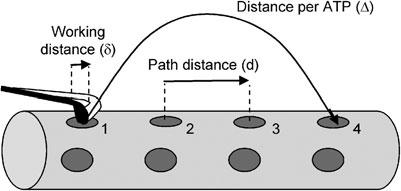
\includegraphics[width=0.8\textwidth]{534.png}
  \caption{Distancias asociadas con un modelo más sofisticado del puente cruzado de actina-miosina. Este puente cruzado se mueve paralelo al eje del filamento y omite dos sitios de unión potenciales durante un ciclo de hidrólisis. La relación de trabajo es baja en este ejemplo. (Basado en \cite{34})}
  \label{fig:534}
\end{figure}



¿Cuál es la potencia mecánica máxima proporcionada por las piernas durante ejercicios como subir escalones rápidamente? ¿Cómo se proporciona esto mediante estos puentes cruzados? Asumamos que los músculos de la pantorrilla y del muslo se contraen ambos una distancia de $3\text{ cm}$ durante un paso y calculemos la energía necesaria para realizar esas contracciones requeridas durante un tiempo de paso de $0{,}25\text{ s}$, y por lo tanto la potencia necesaria. Si ambos músculos tienen un diámetro total promedio de $10\text{ cm}$ y el diámetro efectivo de un filamento de miosina es de $20\text{ nm}$, el número de filamentos de miosina en una sección transversal de cada músculo es de aproximadamente $(10\text{ cm})^2/(20\text{ nm})^2 = 2{,}5 \times 10^{13}$, por lo que hay alrededor de $5{,}0 \times 10^{13}$ filamentos en sección transversal para ambos músculos. Hay seis cadenas de cadenas laterales por filamento de miosina (como se observa en la Fig. 5.6), por lo que hay $3{,}0 \times 10^{14}$ puentes cruzados en sección transversal.

Si la unión/desprendimiento de cada puente cruzado contrae la cadena en $5{,}3\text{ nm}$, debido a que cada músculo se contrae $3\text{ cm}$, el número total de uniones/desprendimientos de puentes cruzados durante el movimiento es de aproximadamente $(3{,}0 \times 10^{14})(3\text{ cm}/5\text{ nm}) = 1{,}8 \times 10^{21}$. Si cada movimiento de puente cruzado requiere la hidrólisis de una molécula de ATP, la cual libera $14\text{ kcal/mol} = 9{,}7 \times 10^{-20}\text{ J}$ (como se discute en el Cap. 6), la cantidad de energía necesaria es de $\sim (1{,}8 \times 10^{21})(9{,}7 \times 10^{-20})\text{ J} = 175\text{ J}$. Si esta energía se utiliza en $0{,}25\text{ s}$, la potencia es de $175\text{ J}/0{,}25\text{ s} = 700\text{ W}$. Esto es consistente con las potencias metabólicas requeridas para actividades vigorosas como subir escalones (Problema 5.39 y Cap. 6). Tenga en cuenta que parte de la incertidumbre en la respuesta final se debe a la estimación muy aproximada de las secciones transversales efectivas de los músculos utilizados.

\subsection{Modelo estadístico de la curva de fuerza-velocidad de Hill (Tema avanzado)}

Un modelo estadístico de los puentes cruzados en el modelo de filamentos deslizantes de la curva de fuerza-velocidad de Hill reproduce dicha curva y concuerda con los estudios experimentales mejor que esta (cuando se adapta para fibras musculares). Aquí y en los problemas daremos una visión general de la derivación de este modelo de Huxley; el análisis detallado supera el nivel de este texto y se puede encontrar en \cite{19, 32, 36, 37, 38, 40, 41, 53}. Este modelo incluye los puntos clave pero no todos los detalles del modelo de filamentos deslizantes.

Considere el puente cruzado en la Fig. 5.31 \cite{41}. Centrémonos en cómo interactúa la cabeza de miosina con una sola molécula de actina, digamos la etiquetada como $x$, pero ahora dejemos que $x$ se refiera a la coordenada de esta molécula de actina, referida a la cabeza de miosina (lateralmente, a lo largo del eje $x$) para una configuración relajada. Durante el deslizamiento, el valor de $x$ disminuye y la velocidad de contracción es $v = -dx/dt$ (o $-\partial x/\partial t$). Llamemos $n(x)$ a la fracción de moléculas de actina con desplazamiento $x$ con puentes cruzados unidos. Se puede formar un nuevo puente cruzado unido solo si no existe un puente cruzado (lo cual tiene probabilidad $1 - n(x)$) y esto puede ocurrir a una tasa $f(x)$. Un puente cruzado unido puede desprenderse si existe (lo cual tiene probabilidad $n(x)$) y esto puede ocurrir a una tasa $g(x)$. Por lo tanto, el cambio total de la densidad de puentes cruzados con el tiempo, $dn/dt$, es $(1 - n(x)) f(x) - n(x) g(x)$. Esto se debe a cambios que dependen del tiempo explícitamente y a cambios que dependen del tiempo implícitamente debido al deslizamiento. Utilizando la regla de la cadena, esto es $dn/dt = \partial n/\partial t + (\partial n/\partial x)(\partial x/\partial t)$, y la combinación de estos componentes conduce al modelo de Huxley:
\begin{equation}
\frac{\partial n(x, t)}{\partial t} - v(t) \frac{\partial n}{\partial x} = (1 - n) f(x) - n g(x).
\label{eq:5.31}
\end{equation}

Si la fuerza de restauración para un desplazamiento dado $x$ es $r(x)$ ($= kx$ para un modelo de resorte), la tensión (o fuerza) ejercida por el músculo es
\begin{equation}
T = N \int_{-\infty}^{\infty} r(x) n(x, t) dx,
\label{eq:5.32}
\end{equation}
donde $N$ es el número total de puentes cruzados (unidos y no unidos).

Hasta ahora la solución es válida para cualquier variación temporal. Para condiciones de estado estacionario con el filamento deslizándose a velocidad constante $v$ y $\partial n/\partial t = 0$, como se debe suponer al utilizar la curva de fuerza-velocidad de Hill, (\ref{eq:5.31}) se reduce a
\begin{equation}
-v \frac{dn(x)}{dx} = (1 - n(x)) f(x) - n(x) g(x).
\label{eq:5.33}
\end{equation}

Para velocidades muy bajas (condiciones isométricas), el lado izquierdo se aproxima a $0$ y se desarrolla la tensión máxima, y utilizando (\ref{eq:5.32}):
\begin{equation}
T_{\text{max}} = N \int_{-\infty}^{\infty} r(x) \frac{f(x)}{f(x) + g(x)} dx.
\label{eq:5.34}
\end{equation}

Esta solución puede producir la curva de fuerza-velocidad de Hill, pero no presenta las deficiencias asociadas con el uso de ese modelo. Un modelo con las funciones de tasa seleccionadas de manera que se pueda resolver analíticamente se analiza en los Problemas 5.32--5.37. Se pueden utilizar opciones más sofisticadas de $f(x)$ y $g(x)$ para modelar músculos utilizando el modelo de tipo Huxley como el elemento contráctil en el modelo muscular de fibra de Hill \cite{41}.

Este modelo de Huxley asume que cada cabeza de miosina se une a un sitio de actina dado, debido a que los otros sitios están lejos. En un modelo de unión mejorado y más generalizado \cite{41}, la miosina se puede unir a cualquier sitio de actina, los cuales están separados en el filamento delgado por $\Delta x$, modificando (\ref{eq:5.31}) para llegar a:
\begin{equation}
\frac{\partial n(x, t)}{\partial t} - v(t) \frac{\partial n}{\partial x} = \left( 1 - \sum_{j=-\infty}^{\infty} n(x + j \Delta x, t) \right) f(x) - n g(x).
\label{eq:5.35}
\end{equation}
La suma se puede convertir en una integral para obtener el modelo continuo de sitios de unión más simple.

\section{Titina}

La molécula de titina es el tercer filamento en el sarcómero, además de los filamentos gruesos y delgados, y es responsable de la respuesta elástica y viscoelástica de los sarcómeros \cite{44, 45, 46, 49, 56}. En ciertos aspectos, es tan importante para la función de los músculos como lo son los dos filamentos activos. La titina es una sola proteína de $\sim 1\ \mu\text{m}$ de largo que se extiende a través del medio sarcómero, formando una estructura similar a una red alrededor de los filamentos gruesos y delgados, anclándose en el disco Z (o línea Z) (Fig. 5.7), extendiéndose como un resorte a través de la banda I y luego uniéndose a lo largo del filamento grueso hasta la banda M. (El esquema que muestra la titina en la Fig. 5.18 es demasiado simple). Cada molécula de titina está unida a la molécula de titina del sarcómero adyacente en el disco Z y a la titina del medio sarcómero opuesto en la banda M para formar un filamento contiguo a lo largo de la miofibrilla. Las propiedades elásticas y viscoelásticas de la titina se deben a esa parte en la banda I.

Solo la sección de la titina en la región I es completamente extensible. Esta sección tiene un dominio PEVK, el cual incluye residuos de aminoácidos de prolina (P), glutamato (E), valina (V) y lisina (K), flanqueado por secciones similares a inmunoglobulina (Ig) (y a veces también por otras secciones), una de las cuales es proximal (al anclaje del disco Z en el borde del sarcómero) y otra que es distal; estas incluyen del orden de $100$ dominios Ig plegados enlazados en serie.

Más generalmente, existen isoformas de titina N2A (tipos de titina) que se encuentran en los sarcómeros del músculo esquelético e isoformas N2B y N2BA en los sarcómeros del músculo cardíaco, siendo estas últimas relativamente más largas y más flexibles (o complacientes) dentro de la banda I. Todas ellas tienen secciones PEVK flanqueadas por secciones Ig, pero también hay secciones N2A en la titina N2A, secciones N2B en la titina N2B, y secciones tanto N2A como N2B en la titina N2BA (Fig. 5.35). Estas cuatro regiones tienen diferentes propiedades mecánicas. Los segmentos N2A/N2B y PEVK son secuencias de tipo ovillo aleatorio flexible (\textit{random-coil}) con diferente flexibilidad, y confieren una respuesta elástica. Los dominios Ig proximales y distales se pueden enderezar y también se pueden desplegar y replegar (siendo mayor la resistencia mecánica a esto en la región distal), y confieren una respuesta viscoelástica, así como una respuesta elástica.

\begin{SCfigure}[0.75][htbp]
  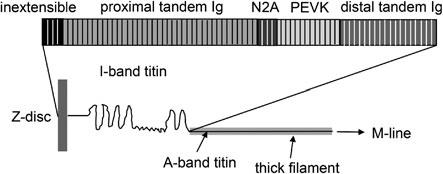
\includegraphics[width=0.6\textwidth]{535.png}
  \caption{Esquema de la región de la banda I en la titina de músculos esqueléticos (para la isoforma esquelética N2A). (Basado en \cite{22})}
  \label{fig:535}
\end{SCfigure}



% Control de Calidad: 19 párrafos origen -> 19 párrafos salida. Mapeo 1:1 verificado. Sin omisiones.

En la titina cardíaca, la tasa característica de despliegue para los dominios Ig es de $\sim 3{,}3 \times 10^{-3}\text{/s}$ y la tasa de repliegue es de $\sim 0{,}3\text{/s}$ \cite{45}. Las energías de plegado/desplegado ($\sim 4\text{ pN}$) y las distancias de un solo dominio Ig en la titina son del mismo orden que las de un puente cruzado de filamento grueso y delgado, como se observa al examinar una sola molécula de titina. Dentro del régimen fisiológico normal, bajo tensión la titina se extiende primero enderezando los enlaces interdominio en las regiones Ig y, a fuerzas más altas, mediante la elongación de los segmentos N2A/N2B y PEVK. Solo para fuerzas mucho mayores, por lo general por encima del rango fisiológico, se extienden los dominios Ig proximales y luego los distales; dicho despliegue puede ser una forma de prevenir el daño muscular a niveles altos de fuerza.

Para cada tipo de titina, las diferentes secciones tienen longitudes distintas en los diferentes tipos específicos de músculos. Esta diferencia en la composición del filamento de titina en diferentes músculos es responsable de las rigideces pasivas variables de distintos músculos, con formas más cortas (isoformas) que conducen a respuestas más rígidas y a una mayor tensión pasiva tras la extensión, y formas más largas que conducen a respuestas más flexibles (o complacientes) y a una menor tensión pasiva. La titina también puede servir como una regla molecular de la longitud del sarcómero.

\section{Coordinación de los músculos}

Muchos músculos están involucrados en la mayoría de los tipos de movimiento \cite{28, 29, 30}. A veces trabajan juntos y son agonistas o protagonistas, o se ayudan mutuamente de otras maneras y son sinergistas (ambos mayormente en fase), y a veces son antagonistas (y fuera de fase). La discusión de los músculos involucrados en el caminar, correr y saltar en el Cap. 3 (Figs. 3.3, 3.4, 3.5, 3.12, 3.13 y 3.31; Tablas 3.1, 3.2, 3.3) y anteriormente en este capítulo proporciona varios ejemplos tanto de protagonistas (por ejemplo, varios flexores de la misma articulación) como de antagonistas (por ejemplo, extensores/flexores de la misma articulación, etc.). La actividad muscular coordinada durante cada fase del ciclo de marcha se muestra para las tres articulaciones sagitales en las Figs. 3.12 y 3.13.

La Figura 5.36 muestra las fuerzas desarrolladas en los músculos sóleo y gastrocnemio en la parte superior de la pantorrilla de un gato que camina como una función del tiempo durante un paso. Ambos están involucrados en este movimiento y necesitan trabajar juntos. Sin embargo, cumplen diferentes funciones: el sóleo (con más fibras musculares ST) para la estabilidad y el gastrocnemio (con más fibras musculares FT) para la fuerza vertical y, como tales, no están exactamente en la misma fase. Esto es evidente en la Fig. 5.37, que grafica cómo evoluciona la fuerza del sóleo en función de la fuerza del gastrocnemio, con el tiempo como una variable implícita. Si trabajaran exactamente en fase, los tres conjuntos de gráficos de fuerza en la Fig. 5.36 verían la misma forma. Sin embargo, la fuerza se desarrolla primero en el gastrocnemio durante un paso y luego, un poco más tarde, se desarrolla la fuerza en el sóleo. Además, a medida que aumenta la velocidad de la marcha, la fuerza desarrollada en el gastrocnemio aumenta en relación con la desarrollada en el sóleo. El gráfico de fuerza en la Fig. 5.38 muestra que el músculo tibial anterior (Fig. 3.5) y el sóleo trabajan fuera de fase durante un paso.

\begin{SCfigure}[1.3][htbp]
  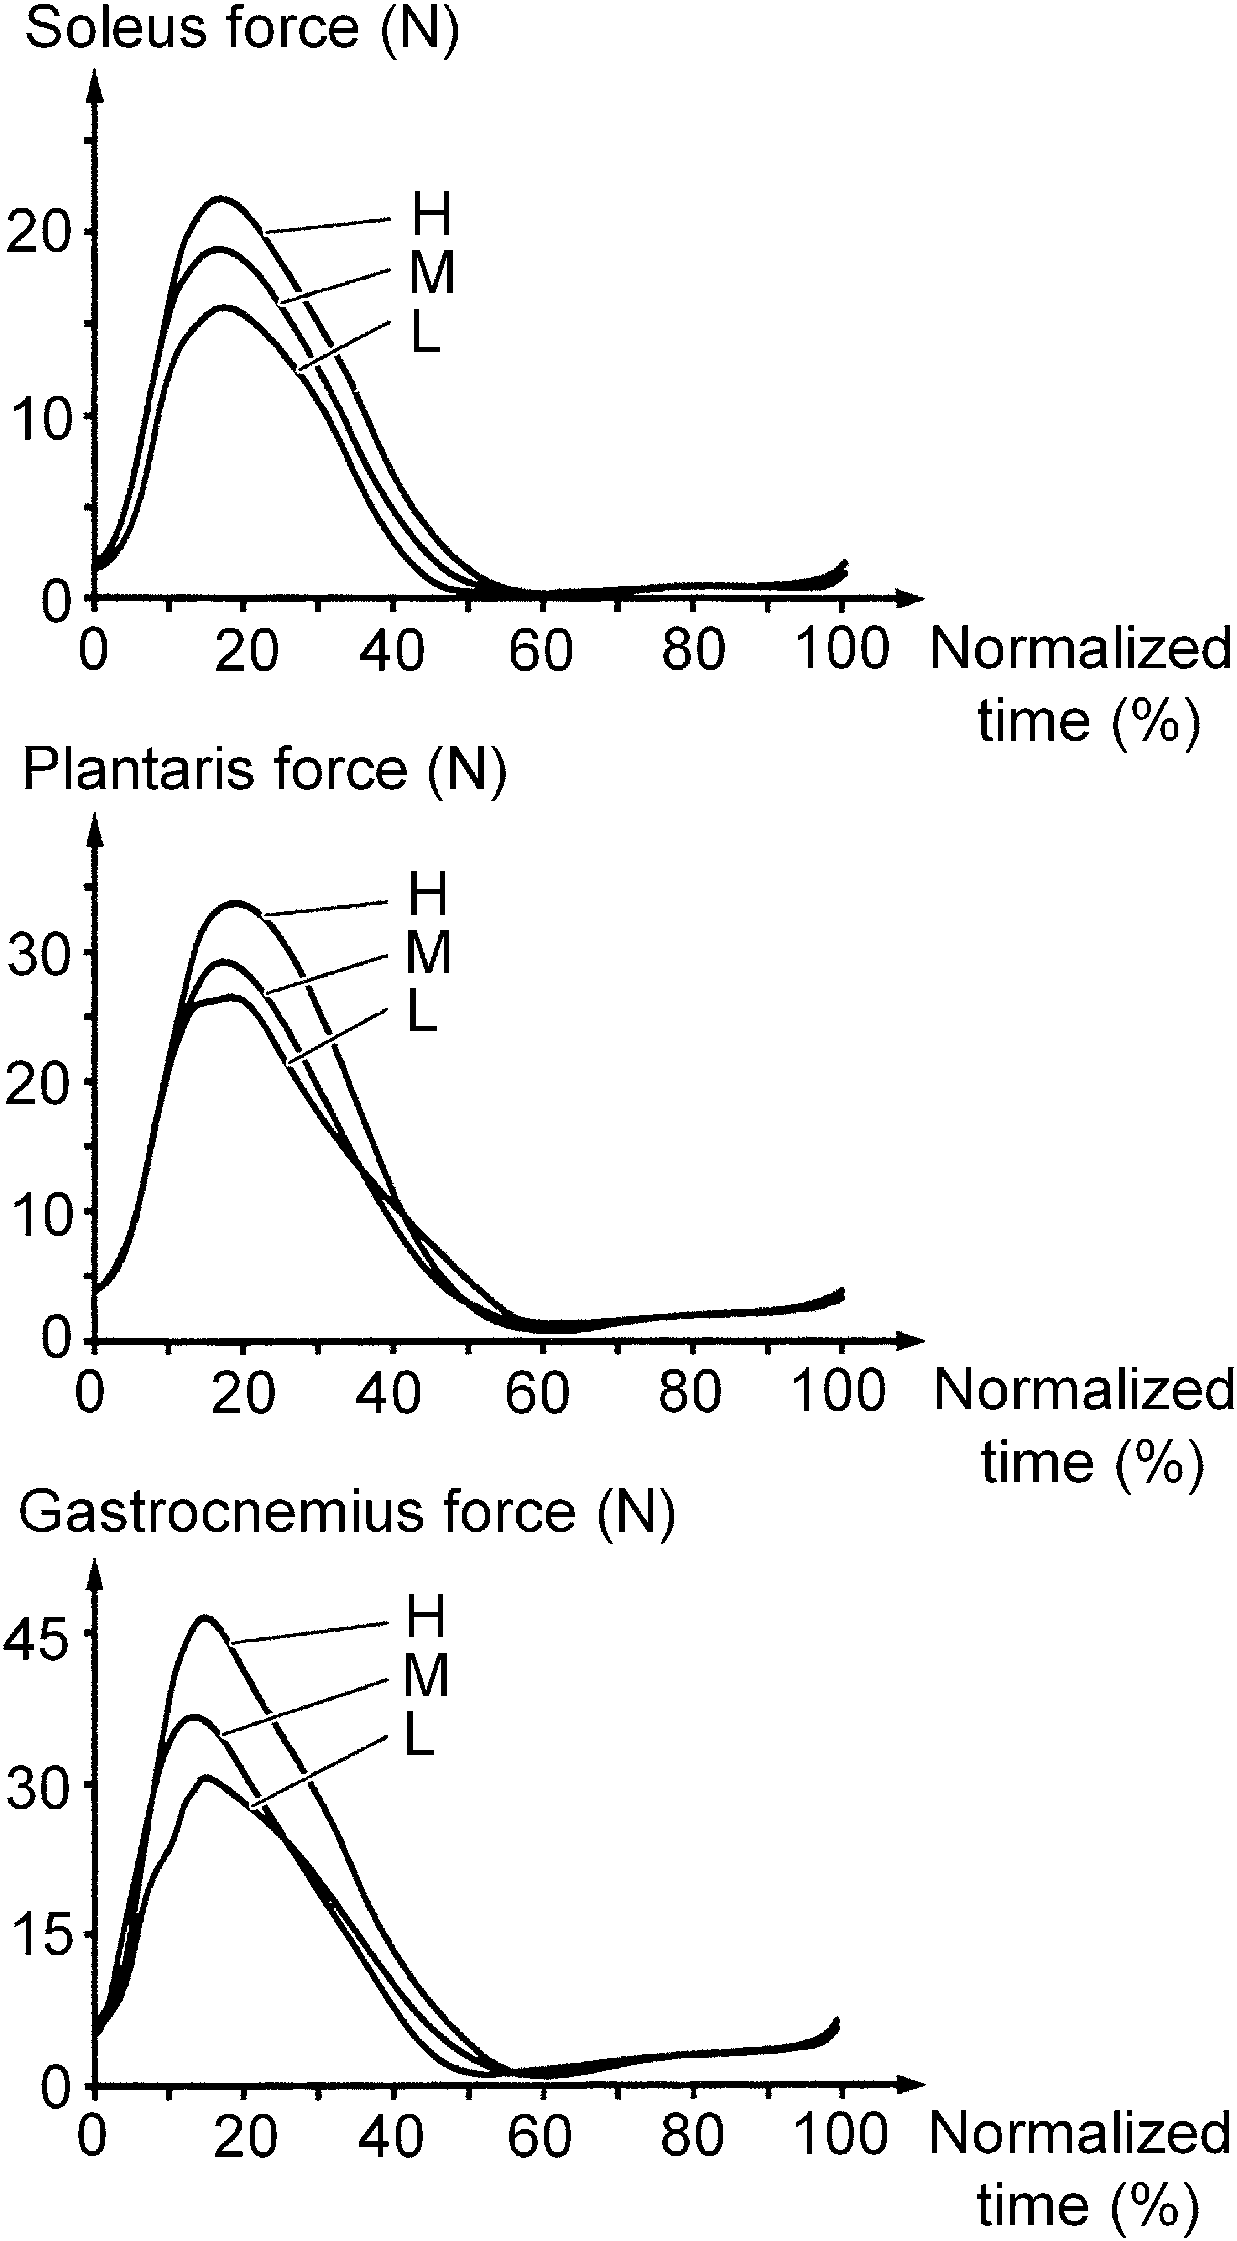
\includegraphics[width=0.35\textwidth]{536.png}
  \caption{Curvas de fuerza frente al tiempo para tres músculos sinergistas en el grupo plantarflexor del tobillo en un gato que camina a $1{,}2\text{ m/s}$, con las fuerzas media (M), más alta (H) y más baja (L) durante 43 ciclos de pasos. (De \cite{59}. Copyright Wiley. Reproducido con autorización. Ver también \cite{30})}
  \label{fig:536}
\end{SCfigure}

\begin{SCfigure}[0.75][htbp]
  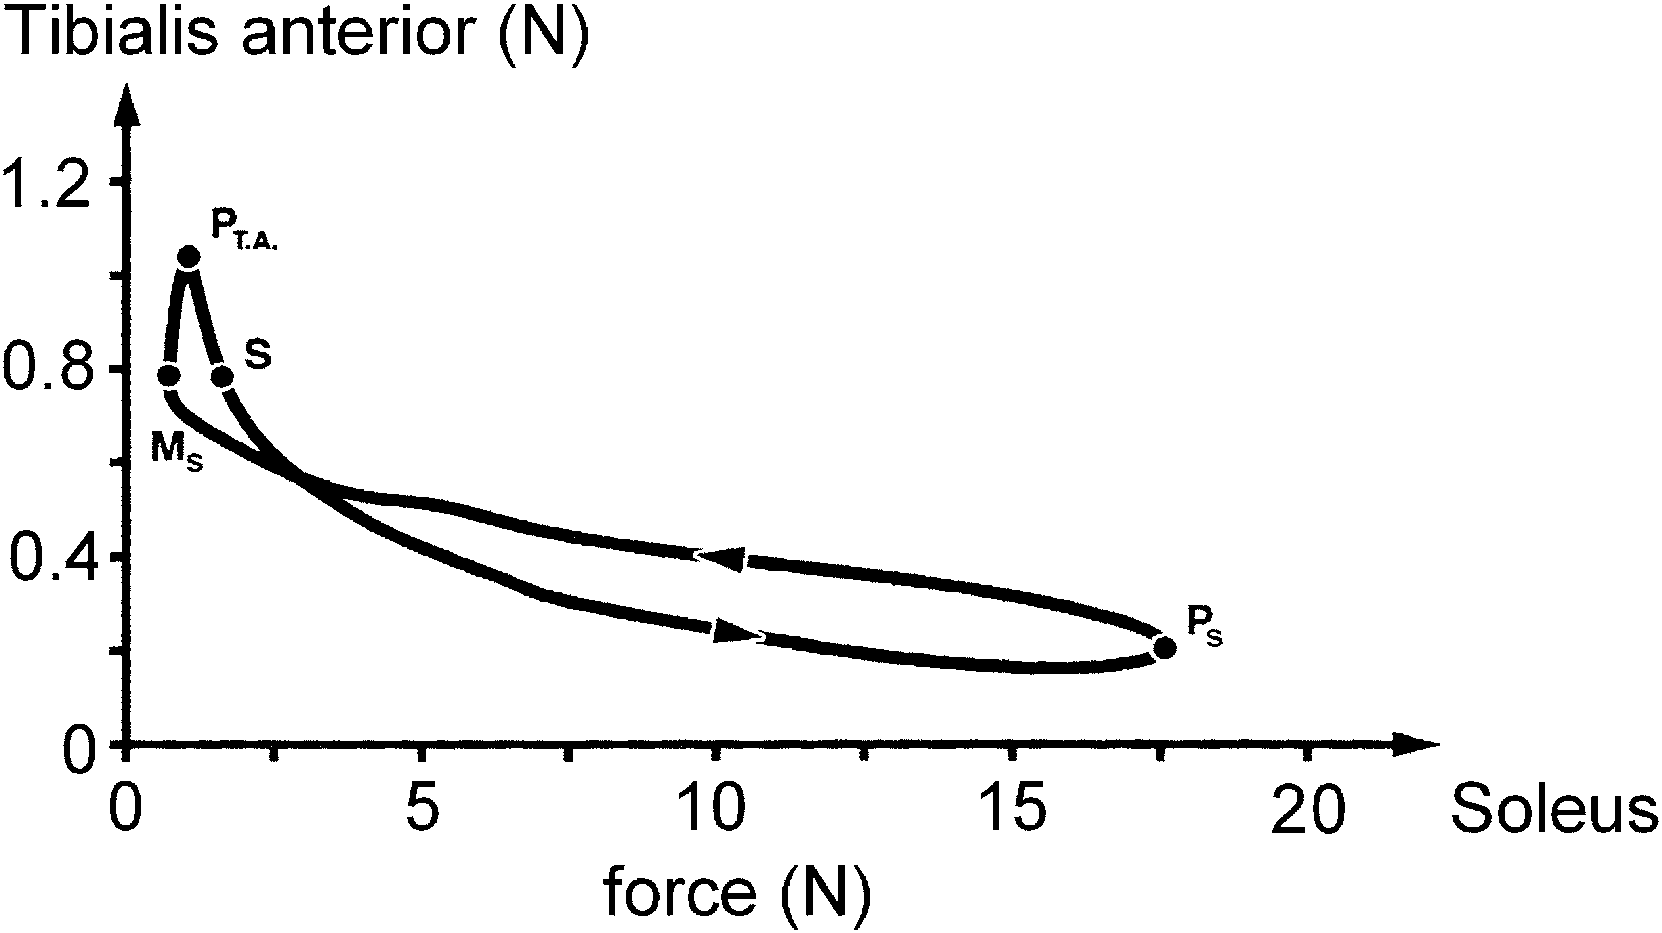
\includegraphics[width=0.6\textwidth]{537.png}
  \caption{Curvas de fuerza frente a fuerza para músculos protagonistas, que muestran la distribución de la fuerza para tres músculos sinergistas en el grupo plantarflexor del tobillo en un gato que camina a $0{,}4$, $0{,}7$ y $1{,}2\text{ m/s}$ y trota a $2{,}4\text{ m/s}$, promediadas sobre 10 ciclos. (De \cite{59}. Copyright Wiley. Reproducido con autorización. Ver también \cite{30})}
  \label{fig:537}
\end{SCfigure}

\begin{SCfigure}[1.0][htbp]
  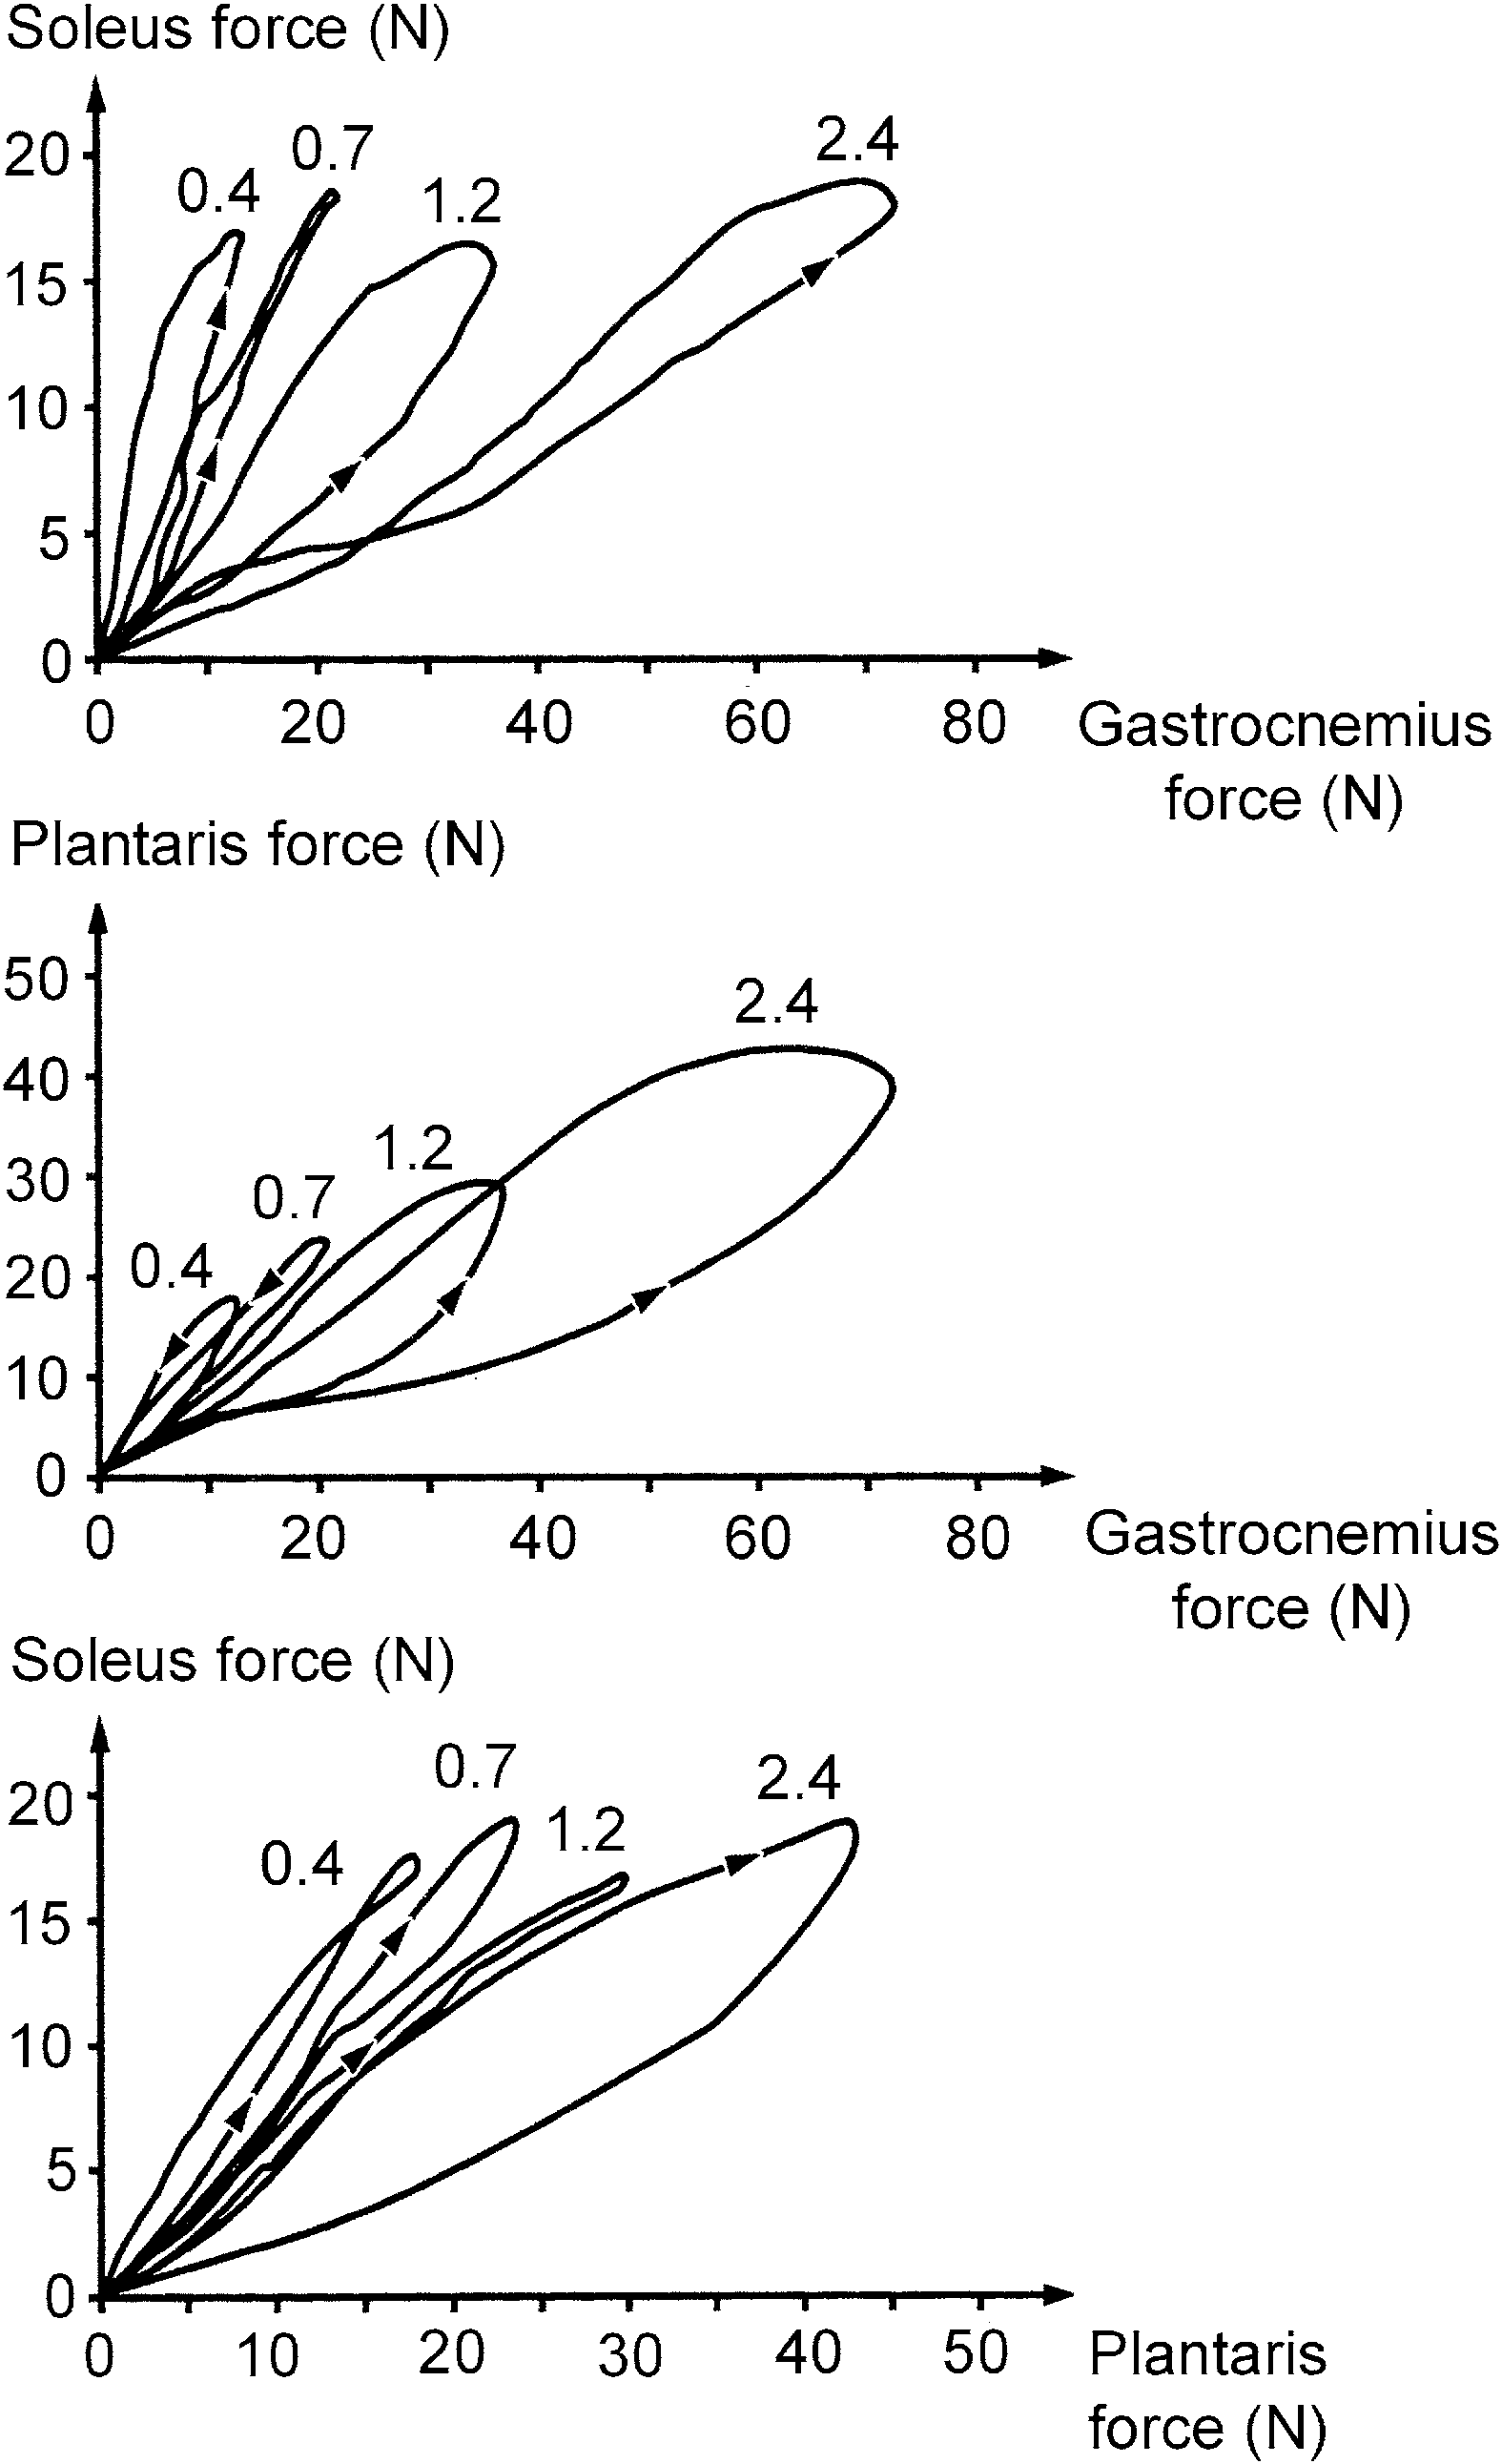
\includegraphics[width=0.45\textwidth]{538.png}
  \caption{Curvas de fuerza frente a fuerza para el par antagonista de los músculos sóleo y tibial anterior en un gato que camina a $0{,}7\text{ m/s}$. (De \cite{59}. Copyright Wiley. Reproducido con autorización)}
  \label{fig:538}
\end{SCfigure}



El ciclismo es otro ejemplo en el que el momento de activación muscular es importante \cite{16}; también es un ejemplo en el que la naturaleza biarticular (de dos articulaciones) de algunos músculos resulta ser muy importante (ver la Fig. 3.2). Al comienzo de la carrera descendente (Fig. 5.39a), la fuerza sobre el pedal debe ser hacia abajo y hacia adelante, para producir torques extensores alrededor de la cadera y la rodilla. El recto femoral biarticular se activa entonces. Este contrarresta parcialmente el efecto de los músculos glúteos mayores activados, para mantener el torque alrededor de la cadera relativamente pequeño, y se suma al efecto de los vastos para hacer que el torque extensor neto alrededor de la rodilla sea grande. (A esto ayuda el brazo de momento mayor del recto femoral alrededor de la rodilla que alrededor de la cadera, como se ve en la figura). A la mitad de la carrera descendente (Fig. 5.39b), la fuerza sobre el pedal debe ser hacia abajo y hacia atrás. La activación de los isquiotibiales biarticulares contribuye al torque extensor positivo neto alrededor de la cadera y al torque flexor neto alrededor de la rodilla, los cuales son necesarios en esta etapa.

\begin{figure}[htbp]
  \centering
  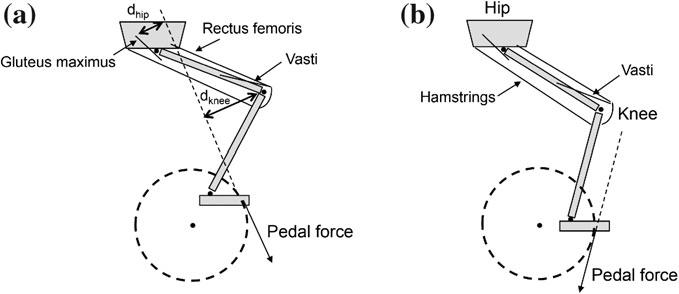
\includegraphics[width=0.8\textwidth]{539.png}
  \caption{Modelo de músculos que cruzan una o dos articulaciones que contribuyen en diferentes etapas del ciclismo. (Basado en \cite{16})}
  \label{fig:539}
\end{figure}



También se requiere coordinación dentro de los músculos complejos. El Problema 5.3 aborda la fuerza resultante sobre el húmero a partir de las diferentes partes del músculo pectoral mayor activadas en fase (Fig. 5.4).

\section{Fuerza muscular y evolución}

La fuerza generalmente se mide de una de tres maneras: (1) la fuerza máxima que se puede ejercer durante una contracción isométrica (la longitud de todo el músculo permanece fija, pero las fibras musculares se acortan), lo cual se denomina contracción voluntaria máxima (MVC, del inglés \textit{maximal voluntary contraction}); (2) la carga máxima que se puede levantar una sola vez, la carga máxima de una repetición (carga 1RM, del inglés \textit{1-repetition maximum}); y (3) el torque de pico durante una contracción isocinética (con acortamiento o alargamiento) \cite{16}. (En tales pruebas y entrenamientos de resistencia, una carga 1RM se define como la carga más alta que se puede mover, y se puede mover solo una vez; una carga 10RM es aquella que se puede mover a lo sumo 10 veces, y así sucesivamente). La Figura 5.40 muestra los ángulos, fuerzas y torques de la rodilla durante ejercicios de rodilla idealizados para estos tres modos. La MVC depende principalmente del tamaño del músculo, mientras que los dos últimos métodos dependen del tamaño del músculo y de la coordinación de la excitación de los músculos. No sorprende que cuantas más repeticiones ($r$) haya en una serie, menor sea la carga máxima ($r\text{RM}$) (Fig. 5.41), aproximadamente como $r\text{RM} = 1\text{RM}(1{,}0278 - 0{,}0278 r)$ \cite{7}.

\begin{figure}[htbp]
  \centering
  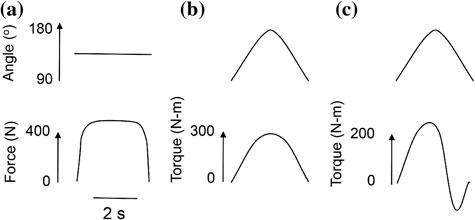
\includegraphics[width=0.8\textwidth]{540.png}
  \caption{Rendimiento idealizado de la medición de la fuerza y el entrenamiento de los músculos extensores de la rodilla para \textbf{a} la contracción voluntaria máxima (MVC), \textbf{b} un levantamiento de una repetición (1RM) y \textbf{c} la contracción isocinética, mostrando el ángulo de la rodilla y la fuerza o torque de la rodilla. La extensión completa de la rodilla es de $180^\circ$. La segunda mitad del movimiento isocinético involucra los músculos flexores de la rodilla. (Basado en \cite{16})}
  \label{fig:540}
\end{figure}

\begin{SCfigure}[0.8][htbp]
  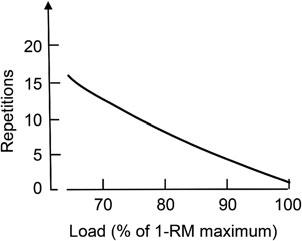
\includegraphics[width=0.55\textwidth]{541.png}
  \caption{La carga máxima que se puede levantar disminuye con un mayor número de repeticiones en la serie. (Basado en \cite{16, 64})}
  \label{fig:541}
\end{SCfigure}



\subsection{Aumento de la fuerza con el entrenamiento}

El $\text{PCA}$ (área de sección transversal fisiológica) de un músculo aumenta con el ejercicio. Este aumento se debe principalmente a incrementos en el área de la sección transversal de las fibras musculares individuales, lo cual se denomina hipertrofia. Alguna vez se pensó que la formación de nuevas fibras, la hiperplasia, no contribuía en absoluto a este aumento, pero ahora unos pocos estudios ---aunque no todos--- han encontrado evidencia de ella en humanos. Con el entrenamiento continuo a una carga dada, la hipertrofia continúa hasta que la fuerza muscular se ajusta a la carga.

Los músculos se pueden fortalecer al vencer cargas mediante la contracción muscular, lo cual es el ejercicio concéntrico, como en el levantamiento de pesas. El movimiento de retorno lento y controlado a dicho ejercicio concéntrico de un músculo dado utiliza la contracción excéntrica del músculo antagonista; este ejercicio excéntrico fortalece estos músculos antagonistas, pero puede provocar daño muscular. Para una carga constante, como la que proporcionan las pesas libres, la carga máxima que se puede utilizar durante el entrenamiento (o levantamiento, etc.) sobre un amplio rango de ángulos articulares corresponde a las fuerzas más bajas alcanzadas por los músculos mucho más cortos y largos que la longitud óptima (Fig. 5.19). Esto no proporciona un entrenamiento muy satisfactorio debido a que la carga está muy por debajo de las cargas que podrían vencerse cerca de la longitud óptima del músculo. Algunos sistemas de entrenamiento varían la carga con el ángulo de la articulación para entrenar el músculo de manera óptima para el rango completo de rotación de la articulación. (¿Puede el entrenamiento mejorarse también ejercitando el músculo cerca de su longitud óptima con menos rotación alrededor de la articulación?)
En el ejercicio isométrico, los músculos intentan contraerse contra una carga inmóvil, por lo que no hay una contracción muscular real; dicho ejercicio no fortalece el músculo a lo largo de su rango de movimiento, afecta solo a las fibras musculares de contracción lenta y no proporciona entrenamiento cardiovascular ni de flexibilidad. El entrenamiento mediante contracciones isométricas no se traduce bien en ganancias de fuerza en actividades donde la longitud del músculo cambia, y se utiliza principalmente para la rehabilitación. El ejercicio bajo condiciones de tensión muscular constante (isotónico) y con una tasa constante de movimiento (isocinético) son menos comunes. Los detalles sobre el entrenamiento se pueden encontrar en \cite{2, 8, 16, 54}.

% Control de Calidad: 10 párrafos origen -> 10 párrafos salida. Mapeo 1:1 verificado. Sin omisiones.

La optimización del desarrollo de la fuerza ocurre con pocas repeticiones a alta resistencia ($6\text{RM}$ o menos). La optimización del desarrollo de la resistencia muscular ocurre con muchas repeticiones a baja resistencia ($20\text{RM}$ o más). La optimización del tamaño muscular ocurre para cargas entre $6\text{RM}$ y $12\text{RM}$, con intervalos cortos ($<90\text{ s}$) entre las series de repeticiones (más de tres). Para más detalles ver \cite{16, 18, 43, 54, 80}.

\subsection{Evolución del músculo con la edad}

En el desarrollo normal, el número de fibras musculares aumenta en el feto y brevemente en el bebé después del nacimiento, duplicándose en los cuatro meses posteriores al parto \cite{2}. Los músculos de contracción lenta y rápida comienzan a diferenciarse en el feto aproximadamente a los siete meses después de la concepción, y al nacer hay aproximadamente el mismo número de fibras de contracción lenta (tipo I) y de contracción rápida (tipo II). Los diámetros de las fibras musculares aumentan durante el crecimiento del niño (Fig. 5.42). Los tiempos de reacción son lentos en niños pequeños y se vuelven más rápidos durante el crecimiento, en parte debido a la toma de decisiones acelerada (Fig. 5.43).

\begin{SCfigure}[0.75][htbp]
  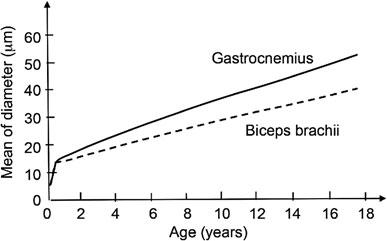
\includegraphics[width=0.6\textwidth]{542.png}
  \caption{Crecimiento del diámetro de la fibra muscular durante la infancia. (Basado en \cite{2})}
  \label{fig:542}
\end{SCfigure}

\begin{SCfigure}[0.8][htbp]
  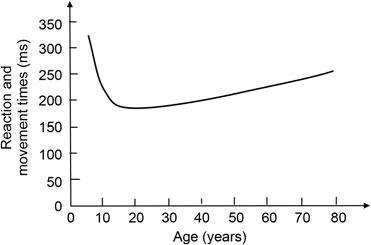
\includegraphics[width=0.55\textwidth]{543.png}
  \caption{Esquema que muestra cómo varían los tiempos de reacción y de movimiento con la edad. (Basado en \cite{2})}
  \label{fig:543}
\end{SCfigure}



Con el avance de la edad se produce una menor fuerza, fatiga más rápida, reacciones más lentas y un peor control de la postura \cite{2, 14, 16}. Para algunos músculos, disminuciones significativas en la fuerza comienzan alrededor de los 60 años (Fig. 5.44a), mientras que para otros comienza a los 20 años y continúa (Fig. 5.44b). En mujeres de 20--89 años, el torque máximo en los músculos extensores de la rodilla (en $\text{N}\cdot\text{m}$) disminuye con la edad (en años) como $224 - 1{,}79(\text{edad})$ y el tiempo de reacción (en $\text{ms}$) aumenta como $153 + 0{,}57(\text{edad})$ \cite{35}. La pérdida de fuerza suele ser mayor que la correspondiente pérdida de masa muscular (por ejemplo, pérdida de fuerza de $\sim 20\text{--}30\%$ para una pérdida de $\sim 15\%$ en la masa muscular del muslo \cite{23}), probablemente debido a la disminución del número de neuronas motoras, la reducción en la tasa máxima a la que se pueden descargar los potenciales de acción (Cap. 12) durante contracciones rápidas, y otros efectos neuronales relacionados con el envejecimiento. Además, la pérdida de área de sección transversal y de masa de las fibras Tipo II es mayor que la de las fibras Tipo I (por ejemplo, $\sim 39\%$ frente a $\sim 19\%$ al comparar el vasto lateral de mujeres de 25 y 67 años \cite{16}), lo que significa que estos músculos más débiles también responden más lento. La Figura 5.43 muestra que los tiempos de reacción y de movimiento se alargan a medida que avanza la edad adulta.

\begin{figure}[htbp]
  \centering
  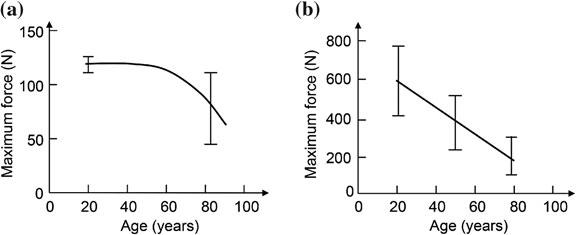
\includegraphics[width=0.8\textwidth]{544.png}
  \caption{Esquema que muestra cómo disminuye con la edad la fuerza muscular promedio MVC para \textbf{a} el músculo de la mano aductor del pulgar y \textbf{b} los músculos cuádriceps femoral, mostrándose también la dispersión de las mediciones individuales. (Basado en \cite{16})}
  \label{fig:544}
\end{figure}



\subsection{Fatiga muscular}

Los análisis de estática y movimiento en los Caps. 2 y 3 asumieron que las fuerzas musculares no cambian con el tiempo, es decir, que nunca hay fatiga muscular. La curva de Rohmert en la Fig. 5.45 caracteriza la disminución hiperbólica en el tiempo de resistencia del control voluntario de un músculo con el nivel de esfuerzo, el cual se expresa como el $\%$ del nivel de fuerza máxima. Aunque no se indica en esta figura, también se espera cierta fatiga por debajo del nivel de esfuerzo del $15\%$. (La Figura 5.41 muestra otro aspecto de la fatiga). Los cambios metabólicos en el músculo y la alteración de la activación contribuyen a la fatiga muscular. La fuerza puede disminuir debido a varios factores metabólicos que dificultan la formación y el desprendimiento de puentes cruzados, incluyendo la formación de ácido láctico, el aumento de fosfato y la disminución de la PCr (fosfocreatina) en las fibras (ver el Cap. 6); el agotamiento de ATP no es dominante. El aumento de la presión intramuscular por encima de la presión arterial máxima (presión sistólica, Cap. 8) restringe el flujo sanguíneo, lo que limita el flujo de oxígeno (es decir, isquemia) al músculo y la eliminación de productos de desecho. En algunos casos, la restricción sanguínea comienza al $10\text{--}20\%$ del nivel de contracción voluntaria máxima; algunos músculos presentan isquemia por encima del $50\%$ de este nivel. La alteración de la activación de los músculos puede deberse a varios factores, como la fatiga central ---la motivación de uno--- y la fatiga periférica ---el fallo del control neuronal de los músculos---. Las fibras musculares Tipo I y IIA resisten la fatiga porque están rodeadas por una rica red de capilares. Los músculos utilizados para mantener la postura, como los músculos sóleo en la pierna inferior, contienen una gran fracción de fibras Tipo I. Los músculos que tienen una ráfaga corta de actividad extrema, como el músculo gastrocnemio, tienen menos necesidad de ser resistentes a la fatiga.

\begin{SCfigure}[0.9][htbp]
  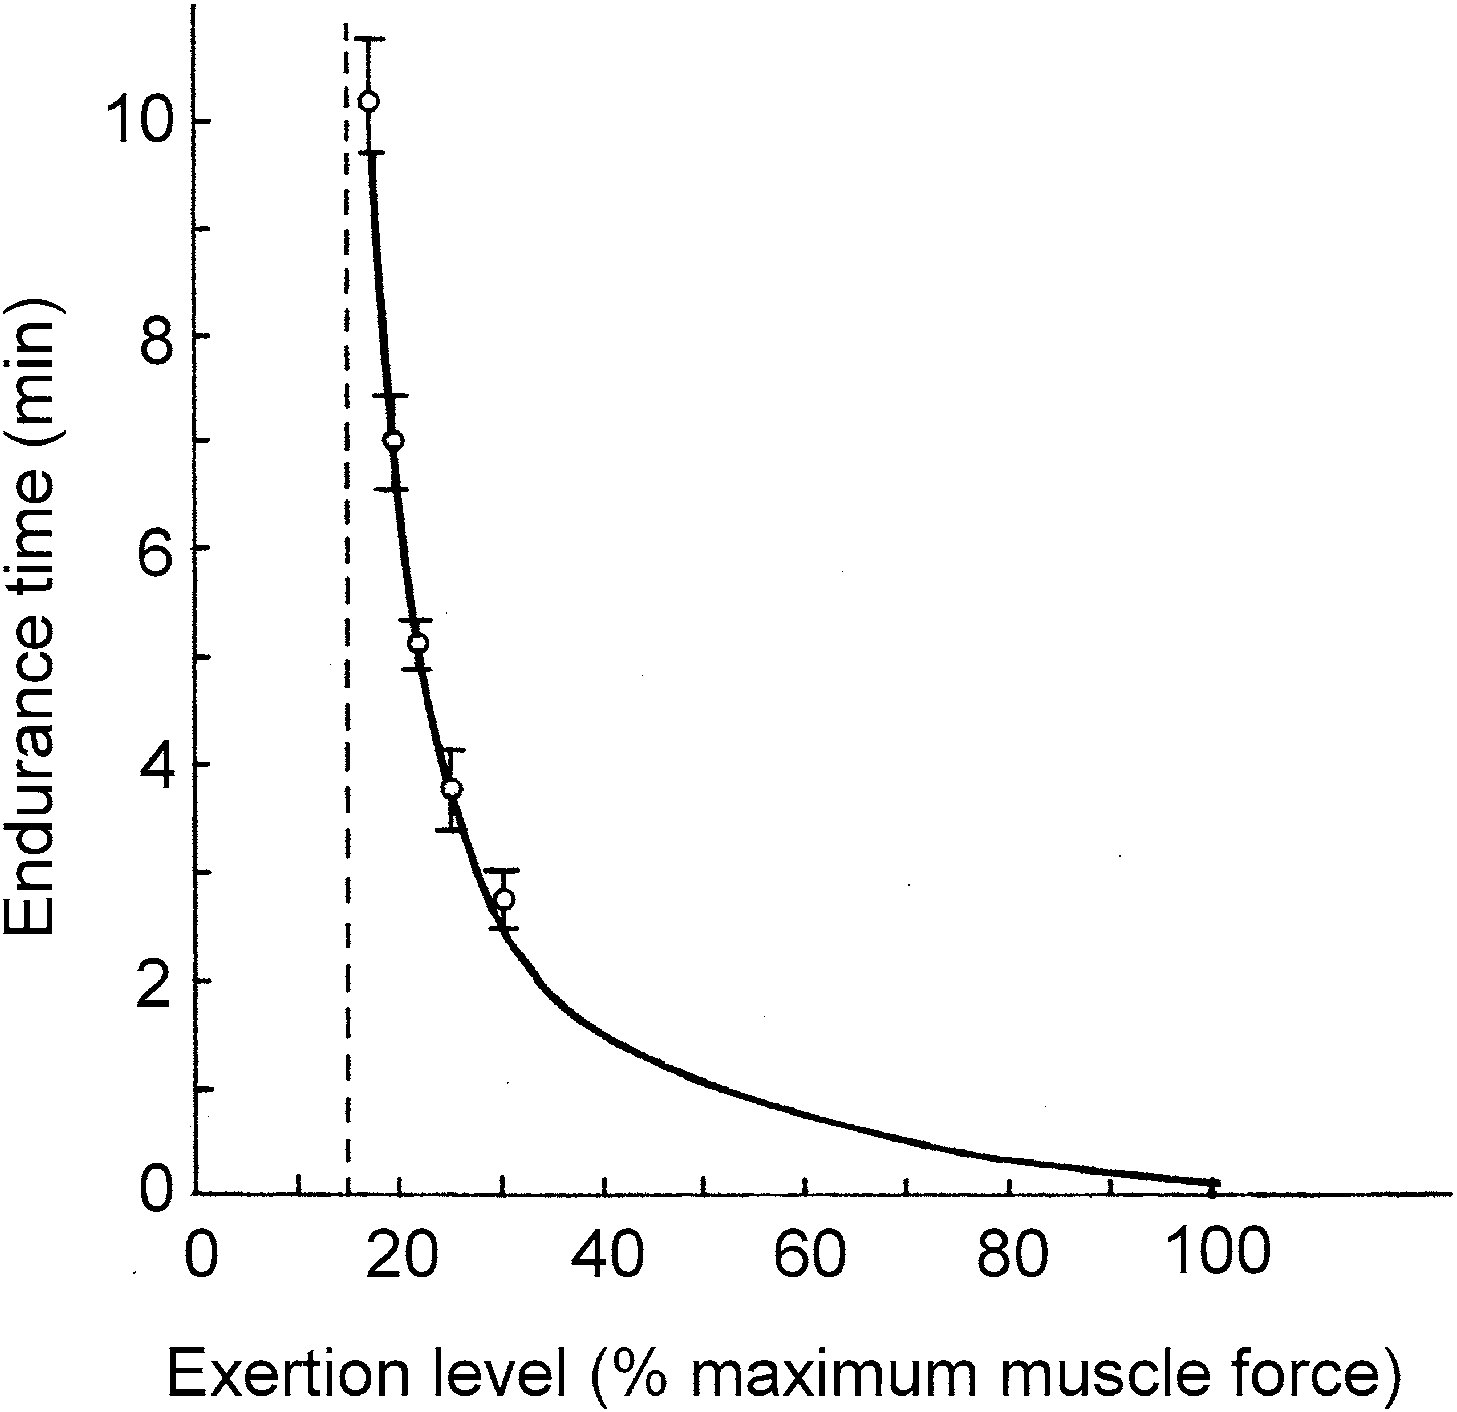
\includegraphics[width=0.5\textwidth]{545.png}
  \caption{Curva de Rohmert para la resistencia muscular estática, mostrándose los puntos de $\pm 1$ DE (desviación estándar). (De \cite{9}, adaptado de \cite{72}. Reimpreso con autorización de Wiley)}
  \label{fig:545}
\end{SCfigure}



\section{Resumen}

La función de los músculos se puede entender analizando su subestructura en términos de fibras, sarcómeros y la estructura de filamentos de los sarcómeros. Las fuerzas desarrolladas por un músculo se pueden modelar como una función de la longitud total del músculo y de la velocidad de contracción. Los modelos mecánicos, similares a los desarrollados en el Cap. 4, se pueden utilizar para examinar las consecuencias de la estimulación eléctrica de los músculos. Sobre una base nanoscópica, las fuerzas desarrolladas por los músculos se pueden entender y modelar en términos de los puentes cruzados entre los filamentos de miosina y actina, y en términos de la respuesta pasiva de la titina.

\section*{Problemas}

\subsection*{Músculos y fuerzas}

\begin{enumerate}

\item[5.1] Existe una fuerza vertical normal promedio de $1710\text{ N}$ ($2{,}7\times$ el peso corporal) en el único pie de un atleta en contacto con el suelo durante la carrera, pero un promedio de solo $715\text{ N}$ en cada pie (y $1430\text{ N}$ de fuerza vertical total con ambos pies $= 2{,}3\times$ el peso corporal) cuando este mismo atleta realiza un salto vertical. ¿Es posible esta diferencia? Cualitativamente, ¿por qué es razonable o irrazonable? (Considere únicamente cómo contribuyen a estas observaciones los rangos de longitud de los músculos en estas actividades. Las Referencias \cite{3} y \cite{4} sugieren que la estimulación de los músculos durante el estiramiento que ocurre inmediatamente antes de la contracción al correr, pero no al saltar, contribuye a esta observación. Esto también es consistente con la observación de que la acción de bajar y subir antes de un salto de altura conduce a saltos más altos).

\item[5.2] (a) ¿Sugieren los datos presentados en la Fig. 5.46 que la fuerza de los músculos varía linealmente con sus áreas de sección transversal, como se asume en el texto? (b) Si es así, ¿cuál es la constante de proporcionalidad? (c) ¿Cómo difiere para hombres y mujeres?

\begin{figure}[htbp]
  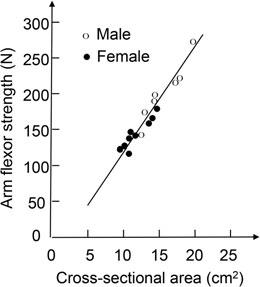
\includegraphics[width=0.55\textwidth]{546.png}
  \caption{La fuerza de los músculos flexores del brazo para hombres y mujeres frente al área de sección transversal del músculo. (Utilizando datos de \cite{39}). Para el Problema 5.2}
  \label{fig:546}
\end{figure}



\item[5.3] Las fibras del músculo pectoral mayor convergen en la parte proximal del húmero. Con el húmero apuntando hacia abajo, las múltiples fibras se pueden modelar como una componente clavicular que ejerce una fuerza de $224\text{ N}$ a un ángulo de $0{,}55\text{ rad}$ por encima de la horizontal y una componente esternal (en el mismo plano y con el mismo momento) que ejerce una fuerza de $251\text{ N}$ a un ángulo de $0{,}35\text{ rad}$ por debajo de la horizontal. Encuentre la fuerza resultante y el ángulo \cite{16}.

\item[5.4] (a) Demuestre que el área de sección transversal fisiológica ($\text{PCA}$) de un músculo para un músculo de fibras paralelas es $\text{PCA} = (m/Ld)\text{ cm}^2$, donde $m$ es la masa de las fibras musculares, $d$ es la densidad de los músculos ($1{,}056\text{ g/cm}^3$) y $L$ es la longitud de las fibras musculares. (b) Repita esto para músculos pinnados, demostrando que $\text{PCA} = (m \cos \theta / Ld)\text{ cm}^2$, donde $\theta$ es el ángulo de pinnación (el ángulo entre el eje largo del músculo y el ángulo de la fibra).

\item[5.5] Verifique si las dos relaciones en el Problema 5.4 son consistentes con los datos musculares proporcionados en la Tabla 5.4.

\item[5.6] Estimemos cuánto peso puede levantar una persona por encima de su cabeza, con los brazos extendidos. (a) Utilice los datos para la persona de $70\text{ kg}$ en el Cap. 1, y específicamente el volumen del músculo esquelético. Supongamos que todos estos músculos están dispuestos como un cilindro circular recto vertical de altura igual a la suma de las longitudes de las piernas, el torso y los brazos de la persona. Utilice el área de sección transversal resultante y asuma que el músculo esquelético puede ejercer una fuerza de $20\text{ N/cm}^2$ para encontrar la masa que la persona puede levantar. (b) ¿Es razonable este valor? Si no es así, describa cómo cada uno de los siguientes factores puede o no contribuir a un resultado irrazonable: (i) Sus brazos son más delgados que sus piernas, por lo que el área de sección transversal del músculo no es uniforme y el factor limitante sería el eslabón más débil (es decir, el más estrecho). (ii) Los músculos no tienen la longitud asumida y debe considerarse que no son más largos que una fraction de la longitud de un segmento de brazo o pierna. En consecuencia, hay varios músculos en serie. (iii) No todo el músculo esquelético del cuerpo está diseñado para contribuir a este levantamiento. (iv) No todos los músculos involucrados son músculos de fibras paralelas. (v) El valor de $20\text{ N/cm}^2$ es inexacto. (c) Ahora vuelva a evaluar el problema para levantadores de pesas de clase mundial, tanto mujeres como hombres, para sus masas levantadas récord mundial. (Utilice los datos proporcionados en el texto). ¿Qué fracción de su área de sección transversal de músculo esquelético (asumida como uniforme aquí) contribuye eficazmente al levantamiento?

\item[5.7] Aquí se presentan algunos datos para los récords mundiales de levantamiento de pesas (en 2014 para envión o dos tiempos, \textit{clean-and-jerk}) para personas de diferentes masas: para hombres, $169\text{ kg}$ levantados (por un hombre de $56\text{ kg}$), $182\text{ kg}$ ($62\text{ kg}$), $198\text{ kg}$ ($69\text{ kg}$), $210\text{ kg}$ ($77\text{ kg}$), $218\text{ kg}$ ($85\text{ kg}$), $233\text{ kg}$ ($94\text{ kg}$) y $238\text{ kg}$ ($105\text{ kg}$); y para mujeres, $121\text{ kg}$ (por una mujer de $48\text{ kg}$), $131\text{ kg}$ ($53\text{ kg}$), $141\text{ kg}$ ($58\text{ kg}$), $143\text{ kg}$ ($63\text{ kg}$), $158\text{ kg}$ ($69\text{ kg}$) y $163\text{ kg}$ ($75\text{ kg}$). ¿Cómo varía el peso levantado con el peso corporal? (Haga esto por separado para hombres y mujeres). ¿Sigue una ley de potencias? ¿Es sublineal? ¿Cómo se puede explicar esta dependencia?

\item[5.8] ¿Cómo se puede realizar una medición de la fuerza frente a la longitud del músculo con el músculo fijo en ambos extremos (condiciones isométricas), como en la Fig. 5.19? ¿Existe una inconsistencia aquí?

\item[5.9] Supongamos que un músculo fusiforme de longitud $L$ y área de sección transversal fisiológica $\text{PCA}$ está unido a los huesos por tendones de longitud $0{,}9 L$ y área de sección transversal $f(\text{PCA})$ ($f \ll 1$) en cada extremo. Esta longitud total de $2{,}8 L$ se mantiene fija mientras el músculo se contrae un $20\%$ y desarrolla una fuerza correspondiente a $15\text{ N/cm}^2$. Utilice los datos de la Tabla 4.2. (a) Encuentre la deformación unitaria en los tendones. ¿Cómo se compara con el $\text{UPE}$ (energía potencial elástica máxima) para los tendones? (b) Relacione $f$ con $Y$ (módulo de Young) para el tendón. (c) Utilizando el valor de $Y$ de la tabla, compare los diámetros del músculo y de los tendones. (d) Encuentre el esfuerzo en los tendones. ¿Cómo se compara con el esfuerzo límite ($\text{UPE}$) para los tendones?

\item[5.10] (Problema avanzado) Demuestre que los dos modelos de la Fig. 5.14 son matemáticamente equivalentes, con $c_1/(k_1 + k_2) = c_2/k_4$; $k_1 k_2/(k_1 + k_2) = k_3$; $k_2 = k_3 + k_4$; y $(k_2/(k_1 + k_2)) T_{\text{G1}} = T_{\text{G2}}$ \cite{53}.

\item[5.11] (a) Se estima que la potencia máxima que se puede obtener de los músculos esqueléticos es de $\sim 250\text{--}500\text{ W/kg}$ para condiciones isotónicas y $1{,}75\times$ esta con preestiramiento \cite{25}. Asuma que durante el lanzamiento de béisbol el trabajo realizado durante la rotación del húmero es de $\sim 132\text{ J}$ en un tiempo de $0{,}034\text{ s}$. Se piensa que los músculos del hombro involucrados en esta rotación tienen una masa de hasta $2{,}16\text{ kg}$ en personas grandes. ¿Cuál es la potencia mecánica asociada con esta rotación del hombro?
(b) Determine esta potencia por unidad de masa de músculo del hombro y compárela con la potencia máxima que se puede obtener de un músculo preestirado.
(c) Si la potencia por unidad de masa disponible del músculo resulta ser menor que este aumento medido de la energía cinética por unidad de tiempo, explique cómo podría ser esto posible \cite{63}.

\item[5.12] Repita el Problema 5.11, incluyendo ahora la dispersión en el rendimiento dada por las desviaciones estándar, siendo el trabajo realizado durante la rotación del húmero de $132 \pm 52\text{ J}$ en $0{,}034 \pm 0{,}013\text{ s}$ \cite{63}.

\item[5.13] Se sabe que las fuerzas musculares máximas son $1{,}75\times$ mayores cuando los músculos se preestiran que bajo condiciones isotónicas. En el texto y en el Problema 5.11, se asumió que este mismo factor se aplica al comparar la potencia específica máxima de los músculos para estas dos condiciones. ¿Qué asume esto?

\subsection*{Tensión muscular frente a la longitud o el tiempo}

\item[5.14] ¿Por qué supone que la Fig. 3.54 representa la longitud total de los músculos y los tendones?

\item[5.15] Utilice los datos de la Fig. 3.54 para determinar si los principales músculos de las piernas utilizados durante el ciclismo están siempre cerca de sus longitudes óptimas (de modo que siempre ejercen fuerzas casi máximas) o si se vuelven mucho más largos o cortos que estas longitudes óptimas durante partes del ciclo (de modo que ejercen fuerzas mucho menores que los máximos). Justifique su respuesta.

\item[5.16] En el ejemplo de lanzar una pelota estudiado en el Cap. 3, asumimos que la fuerza desarrollada por el bíceps braquial no dependía del ángulo entre el brazo y el antebrazo; este ángulo variaba de $180\text{--}0^\circ$ en el primer enunciado del problema y de $135\text{--}45^\circ$ en el segundo. Utilice lo que ahora sabemos sobre cómo varía la fuerza contráctil de un músculo con su longitud para determinar la validez de esa segunda suposición. Asuma que el músculo tiene una longitud de $L_0 = 12\text{ cm}$ en reposo a $90^\circ$, y que la distancia desde la articulación del codo hasta el punto de inserción en el radio es de $4\text{ cm}$ (ver la Fig. 5.47). (Debe basar sus conclusiones en cálculos de la longitud del músculo para varios ángulos; al menos para $0$, $45$, $90$, $135$ y $180^\circ$. Ignore la longitud de los tendones).

\begin{figure}[htbp]
  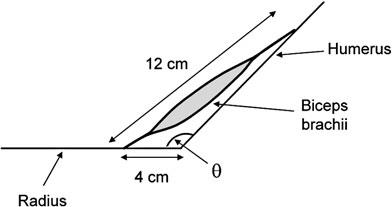
\includegraphics[width=0.8\textwidth]{547.png}
  \caption{Modelo de músculo de fibras paralelas. Para el Problema 5.16}
  \label{fig:547}
\end{figure}



\item[5.17] En los músculos fusiformes (o paralelos), toda la fuerza contráctil del músculo está dirigida a lo largo del eje del tendón y existe una relación entre los cambios en la longitud del músculo y del tendón que depende de las condiciones (contracción isométrica, etc.). En los músculos pinnados y bipinnados, estas relaciones son cualitativamente diferentes. Consulte la Fig. 5.48, que representa un músculo bipinnado en configuraciones relativamente más relajada e inicial (líneas continuas) y relativamente más contraída y final (líneas discontinuas).
(a) En la configuración inicial, la longitud del tendón (hasta el punto donde el músculo se inserta en el tendón, en el punto $B$) es de $8{,}7\text{ cm}$ ($= 2{,}9\text{ cm} + 5{,}8\text{ cm}$ en la figura) y cada fibra muscular tiene $10\text{ cm}$ de longitud y está unida al tendón en un ángulo de $30^\circ$. Supongamos que hay un total de $N$ fibras unidas al tendón cerca de este punto (con un número igual de fibras en ambos lados) y que cada fibra ejerce una fuerza $F_{\text{fibra}}$. Encuentre la fuerza total transmitida al tendón $F_{\text{tendón}}$. (¿Hay fuerza ``desperdiciada'' aquí?)
(b) El músculo se contrae de modo que la longitud del tendón (hasta el punto $C$) es de $2{,}9\text{ cm}$, y el ángulo músculo/tendón es ahora de $60^\circ$. Encuentre la longitud del músculo (ver las líneas discontinuas). Durante esta contracción, ¿qué se ha acortado más, las fibras musculares o el tendón? ¿Es esto bueno o malo para la acción muscular? (¿Contrarresta este efecto, junto con la capacidad de unir más fibras musculares a este tipo de tendón, la fuerza ``desperdiciada'' en la parte (a)?)
(c) Encuentre la fuerza transmitida al tendón después de la contracción en la parte (b) $F_{\text{tendón}}$, asumiendo que la fuerza contráctil de cada fibra muscular sigue siendo $F_{\text{fibra}}$. ¿Cómo ha cambiado la fuerza transmitida al tendón?
(d) Ahora considere el caso más general, en el que reconocemos que la fuerza ejercida por una fibra muscular cambia con la longitud. Supongamos que $F_{\text{fibra}}$ alcanza su máximo a una longitud $L = 8\text{ cm}$, con $F_{\text{fibra}}(L) = F_{\text{máx}}(1 - (L - 8)^2/8)$. Esboce $F_{\text{tendón}}$ a medida que $L$ se contrae desde $10$ hasta $6\text{ cm}$. ¿Alcanza su máximo exactamente a la longitud donde $F_{\text{fibra}}(L)$ alcanza su máximo? ¿Por qué?

\begin{figure}[htbp]
  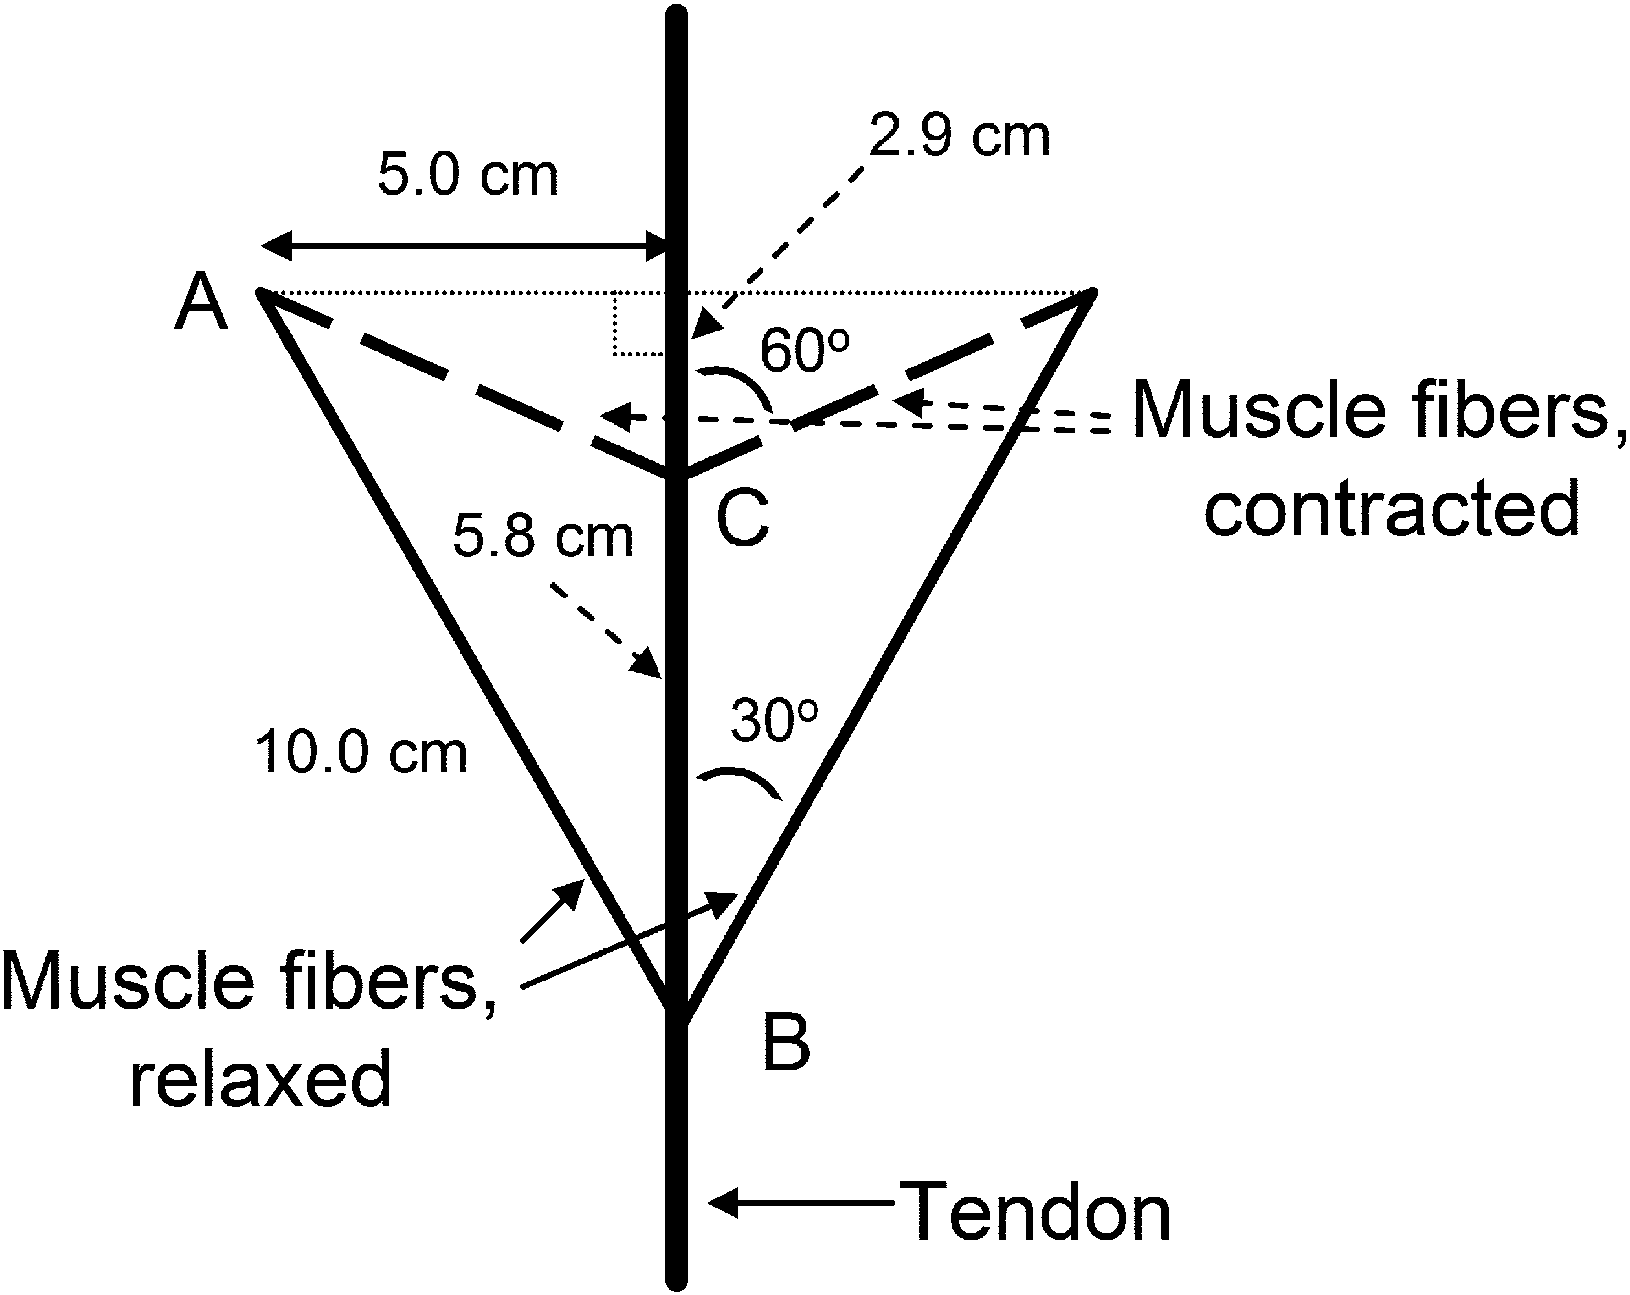
\includegraphics[width=0.7\textwidth]{548.png}
  \caption{Modelo de músculo de fibras bipinnadas. (Basado en \cite{52}). Para el Problema 5.17}
  \label{fig:548}
\end{figure}



\item[5.18] Modelemos la disminución de la fuerza muscular $F$ desde su valor máximo $F_{\text{máx}}$ a una longitud $L_{\text{peak}}$ como una parábola: $F(L) = F_{\text{máx}} - \Delta F((L - L_{\text{peak}})/L_{\text{dec}})^2$. Demuestre que el trabajo realizado por el músculo cuando se contrae desde $L = L_{\text{peak}} + L_{\text{dec}}$ hasta $L = L_{\text{peak}} - L_{\text{dec}}$ es $W = W_0(1 - \Delta F/3F_{\text{máx}})$, donde $W_0 = 2F_{\text{máx}}L_{\text{dec}}$ es el trabajo que el músculo realizaría si la fuerza no cambiara con la longitud \cite{55}.

\item[5.19] Esboce en un solo conjunto de ejes las seis curvas de la Fig. 5.20, cada una como el porcentaje de la fuerza máxima para ese grupo muscular frente al ángulo de tracción (que es el ángulo de la articulación). El eje de ordenadas debe ir de $0$ a $100\%$ (y por supuesto, el $100\%$ representa una fuerza máxima diferente para cada una de las curvas).

\item[5.20] (a) Demuestre que el modelo que utilizamos para el torque que se puede desarrollar en una articulación debido a la contracción muscular, $\tau = \tau_{\text{max}}((\omega_{\text{max}} - \omega)/(\omega_{\text{max}} + G))$, puede derivarse de la curva fuerza-velocidad de Hill (5.21). Esto se expresa en función de la tasa de cambio del ángulo de la articulación durante la flexión, con $\omega = -d\theta/dt$, de modo que $\omega$ es positiva cuando el ángulo se está volviendo más pequeño, y donde $\omega_{\text{max}}$ y $G \sim 3$ son constantes. (Utilizamos esto en los modelos de fuerza de los saltos de altura y de longitud en el Cap. 3).
(b) Explique cómo la relación utilizada para la extensión de la articulación en este modelo del Cap. 3, $\tau = \tau_{\text{max}}$, es un poco diferente de la esperada a partir de la discusión de este capítulo.

\item[5.21] Determine los valores de $T$ y $v$ que maximizan la producción de potencia de un músculo descrito por la ecuación fuerza-velocidad de Hill (5.20) y encuentre la producción de potencia $P_{\text{max}}$ del músculo. Tome $a/T_{\text{max}} = 0{,}25$; recuerde que $P = T v$. (Sugerencia: Debe diferenciar la expresión de la potencia con respecto a $v$ e igualarla a cero. Una forma de hacer esto es resolver primero para $T(v)$ a partir de la ecuación de Hill y expresar $P(v) = T(v)v$. La potencia máxima debería resultar ser aproximadamente $0{,}1 T_{\text{max}} v_{\text{max}}$).

\item[5.22] Utilice el modelo de Hill para una fibra muscular (5.24) para demostrar que $T(t)$ evoluciona como $-T - (T_{\text{max}} + a) \ln((T_{\text{max}} - T)/T_{\text{max}}) = kbt$, para $dL/dt = 0$ (condiciones isométricas), cuando $T(0) = 0$ y $T_{\text{max}}$ es constante \cite{41}. Demuestre que $T$ eventualmente se convierte en $T_{\text{max}}$.

\item[5.23] Utilice el modelo de Hill para una fibra muscular (5.24) para demostrar que $T(t)$ evoluciona como $T_{\text{max}} - T + (T_u + a) \ln((T_{\text{max}} - T_u)/(T - T_u)) = kt(b + u)$, donde $(T_u + a)u = b(T_{\text{max}} - T_u)$, para una fibra muscular inicialmente con $T(0) = T_{\text{max}}$ a la que luego se le permite contraerse a velocidad constante $u = -dL/dt$ \cite{41}. ($T_{\text{max}}$ no cambia). Demuestre que $T$ eventualmente se convierte en $T_u$.

\item[5.24] Utilice el modelo de Hill para una fibra muscular (5.24) para determinar la tensión en una fibra muscular, inicialmente en $T_{\text{max}}$, que se acorta repentinamente desde su valor inicial de $L_0$ en una cantidad $L_1$ en $t = 0$ \cite{41}.
(a) Demuestre que $L(t) = L_0 - L_1(1 - \theta(t))$ y, por lo tanto, $dL/dt = -L_1 \delta(t)$ y (5.24) se convierte en $dT/dt = k(-L_1 \delta(t) + b(T_{\text{max}} - T)/(T + a))$. (Esto utiliza las funciones escalón de Heaviside y delta de Dirac introducidas en el Cap. 4).
(b) Integre esto desde justo antes de $t = 0$ hasta justo después (de $t$ desde $0^-$ hasta $0^+$), para demostrar que $T(0^+) - T(0^-) = -kL_0$, lo que significa que la consecuencia del acortamiento es disminuir la tensión inicial desde $T_{\text{max}}$ hasta $T_{\text{max}} - kL_1$, la cual ahora llamamos $T(0)$.
(c) Demuestre que para $t > 0$, (5.24) se convierte en $dT/dt = kb(T_{\text{max}} - T)/(T + a)$, e intégrelo con $T(0) = T_{\text{max}} - kL_1$ para encontrar $T(t)$. Asuma que $T_{\text{max}}$ no cambia con el tiempo. (Esto da una aproximación a la tensión final de $T_{\text{max}}$ que es más rápida que la observada experimentalmente, incluso con un ajuste de curva óptimo, y esto ilustra una de las limitaciones de la curva fuerza-velocidad de Hill).

\item[5.25] En el ejemplo de lanzar una pelota estudiado en el Cap. 3, asumimos que la fuerza desarrollada por el bíceps braquial no dependía de qué tan rápido varía el ángulo del codo $\theta$ con el tiempo. La Figura 5.28 muestra que esto no es cierto, porque la longitud del músculo y la velocidad de contracción pueden ser importantes y pueden limitar la tensión desarrollada en el músculo. Una forma de abordar esto es volver a analizar el lanzamiento, limitando la tensión del músculo como se indica en esta figura. Explique cómo se puede hacer esto numéricamente.

\item[5.26] En el análisis del lanzamiento de una pelota estudiado en el Cap. 3, asumimos que la fuerza desarrollada por el bíceps braquial puede depender de la longitud del músculo pero no de qué tan rápido varía el ángulo del codo $\theta$ con el tiempo ($d\theta/dt$). Analizamos las limitaciones de ese modelo adoptando un enfoque bastante diferente al utilizado en el Problema 5.25 (y no utilizaremos la Fig. 5.28 explícitamente). Supongamos que $T_{\text{max}} = (20\text{ N/cm}^2)\text{PCA}$, donde $\text{PCA}$ es el área de sección transversal fisiológica de un músculo, y que $v_{\text{max}} = 6 L_0/\text{s}$ para músculos compuestos predominantemente por fibras musculares ST y $v_{\text{max}} = 16 L_0/\text{s}$ para músculos compuestos predominantemente por fibras musculares FT, donde $L_0$ es la longitud de fibra óptima del músculo de interés. (Debido a que los músculos a menudo están compuestos por combinaciones de fibras musculares FT y ST, el $v_{\text{max}}$ apropiado suele estar entre estos valores límite). Suponga también que $a/T_{\text{max}} = b/v_{\text{max}} = 0{,}25$ y utilice los resultados del Problema 5.21. Para cada parte que sigue, considere el caso estudiado en el Cap. 3 de bíceps braquiales de $2\text{ pulgadas}$ de diámetro, para el cual la velocidad de lanzamiento calculada es de $17{,}8\text{ mph}$ (sin gravedad y $\langle \sin \theta \rangle = 1$), y tome $L_0 = 10\text{ cm}$.
(a) Encuentre $a$ y $b$, asumiendo primero músculos FT y luego ST.
(b) Si la pelota sale de la mano a una velocidad de $x\text{ mph}$, la geometría dice que la velocidad de contracción muscular es menor por la proporción de la distancia de inserción del músculo desde el pivote del codo ($4\text{ cm}$) a la distancia de la pelota desde el pivote ($36\text{ cm}$). ¿Cómo se compara esta velocidad de contracción muscular, basada en el cálculo del lanzamiento, con la velocidad máxima de contracción muscular ($v_{\text{max}}$) para músculos FT y ST? Además, ¿cómo se compara con la velocidad de contracción muscular, para ambos tipos de músculos, a la cual se maximiza la potencia generada por el músculo? (Ignore la respuesta de los tendones. ¿Pueden ser importantes?)
(c) Las potencias promedio y de pico necesarias para ser generadas por los músculos para lograr estas velocidades de lanzamiento son de $178\text{ W}$ y $356\text{ W}$, respectivamente, para el bíceps de $2\text{ pulgadas}$ de diámetro utilizando los cálculos cinemáticos realizados en el Cap. 3. Para los músculos FT y ST, calcule la potencia máxima que el músculo puede generar y compare sus respuestas con los valores calculados utilizando la cinemática. Repita esto si asume (incorrectamente) que la fuerza generada por el músculo es $T_{\text{max}}$ independiente de la velocidad de contracción del músculo, de modo que la potencia máxima del músculo sería $T_{\text{max}} v_{\text{max}}$ (lo cual es claramente incorrecto).
(d) ¿Los resultados en (b) y (c) plantean dudas sobre el cálculo en el Cap. 3 (y por qué)? Si es así, ¿invalida esto totalmente el cálculo o significa que después de alcanzar cierta velocidad de contracción muscular se debe incluir la disminución de la fuerza muscular para mejorar el modelo? (Además, note que dado que el bíceps braquial tiene muchas fibras musculares ST, el límite ``FT'' no es muy realista).

\subsection*{Procesos microscópicos y nanoscópicos en los músculos}

\item[5.27] (a) Estime el tiempo que tardan los iones de $\text{Ca}^{2+}$ en difundirse por toda una célula muscular esquelética típica si la célula tiene un diámetro de $200\ \mu\text{m}$ y el coeficiente de difusión de los iones es de $10^{-5}\text{ cm}^2/\text{s}$. Asuma que la liberación de iones ocurre justo fuera de la célula, debido a la llegada de un pulso nervioso allí, y la difusión ocurre en una dimensión transversal de la célula.
(b) ¿Cómo se compara este tiempo con los tiempos de reacción típicos de los músculos?
(c) La señal nerviosa en realidad activa el retículo sarcoplásmico que corre transversalmente a la membrana externa de la célula, en los bordes de la línea Z de cada sarcómero, y los iones de $\text{Ca}^{2+}$ se liberan allí; en consecuencia, la distancia máxima que los iones necesitan recorrer para difundirse por todo el sarcómero es de $2\ \mu\text{m}$. ¿Cuánto tiempo toma esto y parece este tiempo más razonable?

\item[5.28] Estime el número de sarcómeros en su bíceps braquial:
(a) a lo largo de su longitud,
(b) a través de su sección transversal, y
(c) en total.

\item[5.29] Al levantar un peso, un músculo pasa de ser un $25\%$ más corto que su longitud de reposo a un $25\%$ más largo que esta. Si la longitud de reposo del sarcómero es de $2{,}5\ \mu\text{m}$, ¿cuántos golpes de fuerza de puente cruzado de $11\text{ nm}$ ocurren en cada sarcómero durante el levantamiento?

\item[5.30] La Figura 5.33 es la curva de fuerza frente a desplazamiento de una sola molécula de miosina que interactúa con una molécula de actina durante un golpe de fuerza, medida por ``pinzas ópticas''. Dado que el trabajo es la integral de la fuerza sobre la distancia, estime el trabajo realizado por la molécula de miosina durante un golpe de fuerza. (Utilice la línea discontinua y encuentre el área del triángulo). Si la energía disponible a partir de la hidrólisis de ATP en una célula muscular es de $10^{-19}\text{ J}$, calcule la eficiencia de un golpe de fuerza de miosina al utilizar la energía de la hidrólisis de ATP. Esta estimación utiliza la fuerza media. La eficiencia es $\sim 1{,}75\times$ mayor si se realiza una estimación menos conservadora utilizando las fuerzas más altas registradas \cite{17}.

\item[5.31] (a) Si en un solo puente cruzado de actina-miosina se generan $4\text{ pN}$ por puente cruzado y la distancia del golpe de fuerza es de $11\text{ nm}$, como en la Fig. 5.33, demuestre que el trabajo mecánico realizado es de $22\text{ pN}\cdot\text{nm}$. Exprese esto en $\text{J}$ y en $\text{eV}$ ($1\text{ eV}$ (electrón-voltio) $= 1{,}6 \times 10^{-19}\text{ J}$) por puente cruzado, y en $\text{kcal/mol}$ (para un mol de puentes cruzados).
(b) Si la hidrólisis de ATP libera $14\text{ kcal/mol}$ (como se verá en el Cap. 6) y la hidrólisis de una molécula de ATP activa un puente cruzado, ¿qué fracción de la energía disponible se utiliza en trabajo mecánico?

\item[5.32] (Problema avanzado) En el modelo de filamentos deslizantes de Huxley, asuma $f(x) = 0$ para $x < 0$, $f_1 x/h$ para $0 \le x \le h$, y $0$ para $x > h$, y $g(x) = g_2$ para $x \le 0$ y $g_1 x/h$ para $x > 0$. Utilice (5.34) para demostrar que $T_{\text{max}} = Nkh^2 F_1/2$, donde $F_1 = f_1/(f_1 + g_1)$ \cite{41}.

\item[5.33] (Problema avanzado) Utilice el modelo de filamentos deslizantes de Huxley (5.33) en estado estacionario con velocidad de contracción constante $v$, y $f(x)$ y $g(x)$ y la otra notación del Problema 5.32, para demostrar que para estas funciones de tasa $n(x) = F_1(1 - \exp(-V/v)) \exp[(2x/h)G_2(V/v)]$ para $x < 0$, $= F_1[1 - \exp([(x^2/h^2) - 1](V/v))]$ para $0 < x < h$, y $= 0$ para $x > h$, donde la constante $V = (f_1 + g_1)h/2$, la cual tiene unidades de velocidad, y $G_2 = g_2/(f_1 + g_1)$ \cite{41}. (Sugerencia: Haga esto resolviendo por separado la ecuación de Huxley en las tres regiones espaciales, utilizando las formas apropiadas de las funciones de tasa, para llegar a soluciones separadas y luego elija las constantes indeterminadas para hacer que $n(x)$ sea continua en $x = 0$ y $x = h$. Conserve únicamente las soluciones que no tiendan al infinito en la región (es decir, que estén acotadas) dentro de cada rango (y esto significa que la solución para $x > h$ es $n = 0$). Para la región intermedia, utilice una función de prueba $n(x) = A + B \exp(C x^2)$).

\item[5.34] (Problema avanzado) Utilice $n(x)$ y la otra notación de la solución del modelo de filamentos deslizantes de Huxley para las funciones de tasa elegidas en el Problema 5.33 para demostrar que (5.32) se convierte en $T(v) = T_{\text{max}}[1 - (V/v)[1 - \exp(-(V/v))](1 + (v/V)/2G_2^2)]$ \cite{41}. Esta es la ecuación fuerza-velocidad que puede reproducir la curva fuerza-velocidad de Hill.

\item[5.35] (Problema avanzado)
(a) En la predicción del modelo de filamentos deslizantes de Huxley para $T(v)$ del Problema 5.34, $T$ varía desde $T_{\text{max}}$ para $v = 0$ hasta $0$ para una $v = v_{\text{max}}$ dada. Demuestre que si $F_1 = 0{,}812$ y $G_2 = 3{,}919$, entonces $v_{\text{max}} \simeq 4V$.
(b) Dado que $v_{\text{max}} = b T_{\text{max}}/a$ en la curva fuerza-velocidad de Hill, demuestre que con $T_{\text{max}} = 4a$ (el cual es un ajuste común), entonces $V \simeq b$ en esta aplicación del modelo de Huxley \cite{41}. Esto muestra cómo el modelo de filamentos deslizantes de Huxley reproduce los límites de la curva de Hill, y es fácil demostrar que da la misma forma de curva entre estos dos límites.

\item[5.36] (Problema avanzado)
(a) Para $f_1 = 65/\text{s}$, $g_1 = 15/\text{s}$ y $h = 10\text{ nm}$, demuestre que los resultados del modelo de Huxley en el Problema 5.35 predicen una velocidad máxima de acortamiento de $1600\text{ nm/s}$ para cada par de filamentos, lo que significa para cada medio sarcómero, o $3200\text{ nm/s}$ para cada sarcómero \cite{41}.
(b) Si los sarcómeros tienen una longitud de $2{,}5\ \mu\text{m}$ y la longitud del músculo es de $1\text{ cm}$, encuentre qué tan rápido se puede contraer el músculo.

\item[5.37] (Problema avanzado) Grafique los resultados del modelo de Huxley para $T(v)$ del Problema 5.35 en los mismos ejes que la curva fuerza-velocidad de Hill y compárelos.

\subsection*{Energía, potencia, sinergia, entrenamiento y resistencia muscular}

\item[5.38] Utilizando estimaciones razonables de la longitud, velocidad y fuerza por unidad de área del músculo, determine si la estimación de que se generan $\sim 250\text{ W}$ por $\text{kg}$ de músculo activo es razonable.

\item[5.39] Una persona de $75\text{ kg}$ sube escaleras hasta una altura de $50\text{ m}$ en $53\text{ s}$. Determine la tasa metabólica de la persona durante el ascenso, en $\text{W}$ y $\text{kcal/h}$, asumiendo que el proceso tiene una eficiencia del $25\%$. ¿Cómo se relaciona esto con las estimaciones de la energía utilizada en dicho movimiento en el texto? (Ver el Cap. 6 para más información sobre el metabolismo).

\item[5.40] En un gimnasio, usted ejercita su bíceps braquial con un peso constante al intentar levantarlo (es decir, rotando su antebrazo alrededor de su codo). Esboce la tensión máxima frente a la longitud para su bíceps braquial si:
(a) El peso es tan pesado que apenas puede sostenerlo mientras intenta levantarlo.
(b) El peso es tan ligero que puede levantarlo fácilmente.
Para ambos casos, ¿dónde está el peso en su boceto? Describa cuánto cambia la longitud de su músculo durante el ``levantamiento''.

\item[5.41] Durante un ejercicio de curl de antebrazo, el brazo está fijo, digamos a $45^\circ$ respecto a la vertical, y el codo está fijo a medida que rota el antebrazo (y la mano) alrededor del codo (disminuyendo y luego aumentando el ángulo del codo), mientras sostiene un peso en la mano.
(a) Dibuje diagramas que muestren las direcciones y magnitudes de las fuerzas debidas al peso y a su antebrazo, tanto cerca del comienzo de la primera fase del curl (flexión del codo, comenzando con un ángulo del codo de $180^\circ$) como de la segunda fase del curl (extensión del codo, comenzando con $25^\circ$), ignorando primero los músculos que flexionan el codo \cite{16}.
(b) Etiquetando las fuerzas y distancias según sea necesario, encuentre el torque que los músculos de su brazo necesitan suministrar para ambos casos, asumiendo primero únicamente el equilibrio.
(c) Calcule estos dos torques para un humano estándar de $160\text{ lb}$ y $6\text{ pies}$ y un peso de mancuerna de $30\text{ lb}$.
(d) ¿Esperaría que los torques que necesitaría aplicar durante un curl (con movimiento real) sean mayores, iguales o menores que estos valores?

\item[5.42] (a) Dibuje un diagrama de fuerzas para el ejercicio de curl de antebrazo como en el Problema 5.41, con la mano sosteniendo aún un peso como una barra o mancuerna (entrenamiento con carga constante), y determine y esboce el torque alrededor del codo que sus músculos necesitan suministrar para mantener el equilibrio en función del ángulo del codo. En el entrenamiento con carga constante, la magnitud y la dirección de la fuerza debida al peso libre no cambian durante el ciclo del ejercicio.
(b) Repita (a) para una máquina de ejercicio de carga variable en la que se aplica una fuerza (en la mano) normal al antebrazo que puede variar con el ángulo (entrenamiento con carga variable) \cite{16, 54}. ¿Cuál debería ser esa carga variable en función del ángulo para mantener el equilibrio en función del ángulo del codo (y en equilibrio estático)? ¿En qué se diferencia su respuesta de la de (a)?
(c) La cantidad máxima de torque que sus músculos pueden suministrar depende de su longitud y, en consecuencia, del ángulo de la articulación. En el entrenamiento, a menudo se desea llevar los límites de los músculos al extremo hasta cierto punto. ¿Son las características del entrenamiento con carga variable preferibles a las del entrenamiento con carga constante para el entrenamiento de pesas? ¿Por qué?

\item[5.43] La Fig. 5.37 muestra que a medida que un gato camina más rápido, su gastrocnemio desarrolla más y más fuerza, pero su músculo sóleo no. Explique por qué la contribución relativa del músculo gastrocnemio aumenta con la velocidad.

\item[5.44] Usted extiende y luego flexiona repetidamente su brazo (digamos, como para tocar su hombro), con un periodo de $2\text{ s}$. Esboce las fuerzas en su bíceps braquial y tríceps braquial, cada una frente al tiempo, y ambas una frente a la otra (con el tiempo como parámetro implícito).

\item[5.45] Derive una expresión hiperbólica que describa la curva de Rohmert (Fig. 5.45) que relaciona el tiempo de resistencia y el nivel de esfuerzo de un músculo.

\end{enumerate}

\section*{Referencias}

\begin{thebibliography}{99}
  \bibitem{1} H. Abé, K. Hayashi, M. Sato (eds.), \textit{Data Book on Mechanical Properties of Living Cells, Tissues, and Organs} (Springer, Berlín, 1996)
  \bibitem{2} B. Abernethy, V. Kippers, S.J. Hanrahan, M.G. Pandy, A.M. McManus, L. Mackinnon, \textit{Biophysical Foundations of Human Movement}, 3.ª ed. (Human Kinetics, Champaign, 2013)
  \bibitem{3} R. McNeill Alexander, A. Vernon: The dimensions of the knee and ankle muscles and the forces they exert. \textit{J. Hum. Mov. Stud.} 1, 115--123 (1975)
  \bibitem{4} R. McNeill Alexander: \textit{The Human Machine} (Columbia University Press, Nueva York, 1992)
  \bibitem{5} X. Aubert, M.L. Rouquet, J. Van der Elst: The tension-length diagram of the frog's sartorius muscle. \textit{Arch. Int. Physiol.} 59, 239--241 (1951)
  \bibitem{6} S.M. Block, L.S.B. Goldstein, B.J. Schnapp: Bead movement by single kinesin molecules studied with optical tweezers. \textit{Nature} 348, 348--352 (1990)
  \bibitem{7} M. Brzycki: \textit{A Practical Approach To Strength Training}, 2.ª ed. (McGraw-Hill, Nueva York, 1998)
  \bibitem{8} N. Hamilton, W. Weimar, K. Luttgens: \textit{Kinesiology: Scientific Basis of Human Motion}, 12.ª ed. (McGraw-Hill, Nueva York, 2012)
  \bibitem{9} D.B. Chaffin, G.B.J. Andersson: \textit{Occupational Biomechanics} (Wiley, Nueva York, 1984)
  \bibitem{10} D. Chowdhury: Resource letter PBM-1: physics of biomolecular machines. \textit{Am. J. Phys.} 77, 583--594 (2009)
  \bibitem{11} R.M.J. Cotterill: \textit{Biophysics: An Introduction} (Wiley, Nueva York, 2002)
  \bibitem{12} A. Cutts: The range of sarcomere lengths in the muscles of the human lower limb. \textit{J. Anat.} 160, 79--88 (1988)
  \bibitem{13} C.B. Daish: \textit{The Physics of Ball Games} (The English Universities Press, Londres, 1972)
  \bibitem{14} T.J. Doherty: Invited review: aging and sarcopenia. \textit{J. Appl. Physiol.} 95, 1717--1727 (2003)
  \bibitem{15} J. Enderle, S. Blanchard, J. Bronzino: \textit{Introduction to Biomedical Engineering} (Academic, San Diego, 2000)
  \bibitem{16} R.M. Enoka: \textit{Neuromechanics of Human Movement}, 4.ª ed. (Human Kinetics, Champaign, 2008)
  \bibitem{17} J.T. Finer, A.D. Mehta, J.A. Spudich: Characterization of single actin-myosin interactions. \textit{Biophys. J.} 68, 291s--297s (1995)
  \bibitem{18} S.J. Fleck, W.J. Kraemer: \textit{Designing Resistance Training Programs}, 2.ª ed. (Human Kinetics, Champaign, 1997)
  \bibitem{19} L.E. Ford, A.F. Huxley, R.M. Simmons: Tension responses to sudden length change in stimulated frog muscle fibers near slack length. \textit{J. Physiol.} 269, 441--515 (1977)
  \bibitem{20} M.L. Foss, S.J. Keteyian: \textit{Fox's Physiological Basis for Exercise and Sport}, 6.ª ed. (McGraw-Hill, Boston, 1998)
  \bibitem{21} E.L. Fox: \textit{Sports Physiology}, 2.ª ed. (Saunders College, Filadelfia, 1984)
  \bibitem{22} A. Freiburg, K. Trombitas, W. Hell, O. Cazorla, F. Fougerousse, T. Centner, B. Kolmerer, C. Witt, J.S. Beckmann, C.C. Gregorio, H. Granzier, S. Labeit: Series of exon-skipping events in the elastic spring region of titin as the structural basis for myofibrillar elastic diversity. \textit{Circ. Res.} 86, 1114--1121 (2000)
  \bibitem{23} W.R. Frontera, V.A. Hughes, R.A. Fielding, M.A. Fiatarone, W.J. Evans, R. Roubenoff: Aging of skeletal muscle: A 12-yr longitudinal study. \textit{J. Appl. Physiol.} 88, 1321--1326 (2000)
  \bibitem{24} S.C. Gandevia, R.M. Enoka, A.J. McComas, D.G. Stuart, C.K. Thomas: \textit{Fatigue Neural and Muscular Mechanisms}, Advances in Experimental Medicine and Biology, vol. 384 (Plenum, Nueva York, 1995)
  \bibitem{25} B.A. Garner, M.G. Pandy: Estimation of musculotendon properties in the human upper limb. \textit{Ann. Biomed. Eng.} 31, 207--220 (2003)
  \bibitem{26} A.C. Guyton, J.E. Hall: \textit{Human Physiology and Mechanisms of Disease}, 6.ª ed. (Saunders, Filadelfia, 1997)
  \bibitem{27} D.D. Hackney: The kinetic cycles of myosin, kinesin, and dynein. \textit{Ann. Rev. Physiol.} 58, 731--750 (1996)
  \bibitem{28} W. Herzog: Muscle. En \textit{Biomechanics of the Musculo-Skeletal System}, 2.ª ed., editado por B.M. Nigg, W. Herzog (Wiley, Nueva York, 1999), Secc. 2.7, pp. 148--188
  \bibitem{29} W. Herzog, T.R. Leonard: Validation of optimization models that estimate forces exerted by synergistic muscles. \textit{J. Biomech.} 24(S1), 31--39 (1991)
  \bibitem{30} W. Herzog, V. Zatsiorsky, V. Prilutsky, T.R. Leonard: Variations in force-time histories of cat gastrocnemius, soleus, and plantaris muscles for consecutive walking steps. \textit{J. Exp. Biol.} 191, 19--36 (1994)
  \bibitem{31} A.V. Hill: The heat of shortening and the dynamic constants of muscle. \textit{Proc. R. Soc. Lond. Series B, Biol. Sci.} 126, 136--195 (1938)
  \bibitem{32} F.C. Hoppensteadt, C.S. Peskin: \textit{Modeling and Simulation in Medicine and the Life Sciences}, 2.ª ed. (Springer, Berlín, 2002) (La primera edición de 1992 se tituló \textit{Mathematics in Medicine and the Life Sciences})
  \bibitem{33} J. Howard: The movement of kinesin along microtubules. \textit{Ann. Rev. Physiol.} 58, 703--729 (1996)
  \bibitem{34} J. Howard: \textit{Mechanics of Motor Proteins and the Cytoskeleton} (Sinauer, Sunderland, 2001)
  \bibitem{35} S.K. Hunter, M.W. Thompson, R.D. Adams: Reaction time, strength, and physical activity in women aged 20--89 years. \textit{J. Aging Phys. Act.} 9, 32--42 (2001)
  \bibitem{36} H.E. Huxley: Electron microscope studies on the structure of natural and synthetic protein filaments from striated muscle. \textit{J. Mol. Biol.} 7, 281--308 (1963)
  \bibitem{37} H.E. Huxley: The mechanism of muscle contraction. \textit{Science} 164, 1356--1366 (1969)
  \bibitem{38} A.F. Huxley, R.M. Simmons: Proposed mechanism of force generation in striated muscle. \textit{Nature} 233, 533--538 (1971)
  \bibitem{39} M. Ikai, T. Fukunaga: Calculation of muscle strength per unit cross-sectional area of human muscle by means of ultrasonic measurements. \textit{Int. Z. Angew. Physiol.} 26, 26--32 (1968)
  \bibitem{40} J. Keener, J. Sneyd: \textit{Mathematical Physiology} (Springer, Berlín, 1998)
  \bibitem{41} J. Keener, J. Sneyd (eds.): \textit{Mathematical Physiology II: Systems Physiology}, 2.ª ed. (Springer, Berlín, 2009)
  \bibitem{42} K. Kitamura, M. Tokunaga, A.H. Iwane, T. Yanagida: A single myosin head moves along an actin filament with regular steps of $5{,}3\text{ nanómetros}$. \textit{Nature} 397, 129--134 (1999)
  \bibitem{43} W.J. Kraemer, K. Adams, E. Cafarelli, G.A. Dudley, C. Dooly, M.S. Feigenbaum, S.J. Fleck, B. Franklin, A.C. Fry, J.R. Hoffman, R.U. Newton, J. Potteiger, M.H. Stone, N.A. Ratamess, T. Triplett-McBride: ACSM position stand: progression models in resistance training for healthy adults. \textit{Med. Sci. Sports Exerc.} 34, 364--380 (2002)
  \bibitem{44} M.M. LeWinter, H. Granzier: Cardiac titin: a multifunctional giant. \textit{Circulation} 121, 2137--2145 (2010)
  \bibitem{45} H.B. Li, W.A. Linke, A.F. Oberhauser, M. Carrion-Vazquez, J.G. Kerkvliet, H. Lu, P.E. Marszalek, J.M. Fernandez: Reverse engineering of the giant muscle protein titin. \textit{Nature} 418, 998--1002 (2002)
  \bibitem{46} H. Li, J.M. Fernandez: Mechanical design of the first proximal Ig domain of human cardiac titin revealed by single molecule force spectroscopy. \textit{J. Mol. Biol.} 334, 75--86 (2003)
  \bibitem{47} R.L. Lieber, W.M. Murray, D.L. Clark, V.R. Hentz, J. Friden: Biomechanical properties of the brachioradialis muscle: Implications for surgical tendon transfer. \textit{J. Hand Surg.} 30, 273--282 (2005)
  \bibitem{48} R.L. Lieber: Biology and mechanics of skeletal muscle: what hand surgeons need to know when tensioning a tendon transfer. \textit{J. Hand Surg.} 33, 1655--1656 (2008)
  \bibitem{49} W.A. Linke, M. Krüger: The giant protein titin as an integrator of myocyte signaling pathways. \textit{Physiology} 25, 186--198 (2010)
  \bibitem{50} T. Lorenz, M. Campello, M.J. Pitman, L. Peterson: Biomechanics of skeletal muscle. En \textit{Basic Biomechanics of the Musculoskeletal System}, 3.ª ed., editado por M. Nordin, V.H. Frankel (Lippincott Williams \& Wilkins, Filadelfia, 2001), Cap. 6, pp. 148--174
  \bibitem{51} B.R. MacIntosh, R.J. Holash: Power output and force--velocity properties of muscle. En \textit{Biomechanics and Biology of Movement}, editado por B.M. Nigg, B.R. MacIntosh, J. Mester (Human Kinetics, Champaign, 2000), Cap. 11
  \bibitem{52} A.J. McComas: \textit{Skeletal Muscle: Form and Function} (Human Kinetics, Champaign, 1996)
  \bibitem{53} T.A. McMahon: \textit{Muscles, Reflexes and Locomotion} (Princeton University Press, Princeton, 1984)
  \bibitem{54} D.T. McMaster, J. Cronin, M. McGuigan: Forms of variable resistance training. \textit{Strength and Conditioning Journal} 31, número 1, 50--64 (febrero de 2009), \url{http://performancetrainingsystems.net/Resources/FormsofVariableResistanceTraining.pdf}
  \bibitem{55} H.J. Metcalf: \textit{Topics in Classical Biophysics} (Prentice-Hall, Englewood Cliffs, 1980)
  \bibitem{56} A. Minajeva, M. Kulke, J.M. Fernandez, W.A. Linke: Unfolding of titin domains explains the viscoelastic behavior of skeletal myofibrils. \textit{Biophys. J.} 80, 1442--1451 (2001)
  \bibitem{57} K.L. Moore, A.M.R. Agur: \textit{Essential Clinical Anatomy}, 2.ª ed. (Lippincott Williams \& Wilkins, Filadelfia, 2002)
  \bibitem{58} K.L. Moore, A.M.R. Agur: \textit{Essential Clinical Anatomy}, 3.ª ed. (Lippincott Williams \& Wilkins, Filadelfia, 2007)
  \bibitem{59} B.M. Nigg, W. Herzog (eds.): \textit{Biomechanics of the Musculo-Skeletal System}, 2.ª ed. (Wiley, Nueva York, 1999)
  \bibitem{60} M. Nordin, V.H. Frankel (eds.): \textit{Basic Biomechanics of the Musculoskeletal System}, 3.ª ed. (Lippincott Williams \& Wilkins, Filadelfia, 2001)
  \bibitem{61} J.L. Palladino, A. Noordergraaf: Muscle contraction mechanics from ultrastructural dynamics. En \textit{Analysis and Assessment of Cardiovascular Function}, editado por G.M. Drzewiecki, J.K.-J. Li (Springer, Berlín, 1998), Cap. 3, pp. 33--57
  \bibitem{62} T.D. Pollard, S.K. Doberstein, H.G. Zot: Myosin-I. \textit{Annu. Rev. Physiol.} 53, 653--681 (1991)
  \bibitem{63} N.T. Roach, M. Venkadesan, M.J. Rainbow, D.E. Lieberman: Elastic energy storage in the shoulder and the evolution of high-speed throwing in \textit{Homo}. \textit{Nature} 498, 483--486 (2013)
  \bibitem{64} D.G. Sale, D. MacDougall: Specificity in strength training: a review for the coach and athlete. \textit{Can. J. Appl. Sports Sci.} 6, 87--92 (1981)
  \bibitem{65} T.G. Sandercock: Summation of motor unit force in passive and active muscle. \textit{Exerc. Sport Sci. Rev.} 33, 76--83 (2005)
  \bibitem{66} T.G. Sandercock, H. Maas: Force summation between muscles: are muscles independent actuators? \textit{Med. Sci. Sports Exerc.} 41, 184--190 (2009)
  \bibitem{67} T.H. Schiebler: \textit{Anatomie}, 9.ª ed. (Springer, Berlín, 2005)
  \bibitem{68} R.F. Schmidt, F. Lang, G. Thews: \textit{Physiologie des Menschen}, 29.ª ed. (Springer, Berlín, 2005)
  \bibitem{69} T.A. Schroer, M.P. Sheetz: Functions of microtubule-based motors. \textit{Annu. Rev. Physiol.} 53, 629--652 (1991)
  \bibitem{70} J.M. Squire (ed.): \textit{Molecular Mechanisms in Muscular Contraction} (CRC, Boca Raton, 1990)
  \bibitem{71} A. Stalheim-Smith, G.K. Fitch: \textit{Understanding Human Anatomy and Physiology} (West, St. Paul, 1993)
  \bibitem{72} W. von Rohmert: Arbeitsmedizin. Sozial medizin, Arbeitshygiene 22, 118 (1968)
  \bibitem{73} A. Thorstensson, G. Grimby, J. Karlsson: Force-velocity relations and fiber composition in human knee extensor muscles. \textit{J. Appl. Physiol.} 40, 12--16 (1976)
  \bibitem{74} R.D. Vale: The molecular motor toolbox for intracellular transport. \textit{Cell} 112, 467--480 (2003)
  \bibitem{75} P.A. Wahr, J.M. Metzger: Peak power output is maintained in rabbit psoas and rat soleus single muscle fibers when CTP replaces ATP. \textit{J. Appl. Physiol.} 85, 76--83 (1998)
  \bibitem{76} T.L. Wickiewicz, R.R. Roy, P.L. Powel, V.R. Edgerton: Muscle architecture of the human lower limb. \textit{Clin. Orthop. Relat. Res.} 179, 275--283 (1983)
  \bibitem{77} J.J. Widrick, J.G. Romatowski, M. Karhanek, R.H. Fitts: Contractile properties of rat, rhesus monkey, and human type I muscle fibers. \textit{Am. J. Physiol. Regul. Integr. Comp. Physiol.} 272, R34--R42 (1997)
  \bibitem{78} D.R. Wilkie: The relation between force and velocity in human muscle. \textit{J. Physiol.} 110, 249--280 (1950)
  \bibitem{79} D.R. Wilkie: Man as a source of mechanical power. \textit{Ergonomics} 3, 1--8 (1960)
  \bibitem{80} J.H. Wilmore, D.L. Costill: \textit{Physiology of Sport and Exercise}, 3.ª ed. (Human Kinetics, Champaign, 2004)
  \bibitem{81} D.A. Winter: \textit{Biomechanics and Motor Control of Human Movement}, 3.ª ed. (Wiley, Nueva York, 2005)
  \bibitem{82} F.E. Zajac: Muscle and tendon properties, models, scaling, and application to biomechanics and motor control. \textit{Crit. Rev. Biomed. Eng.} 17, 359--411 (1989)
\end{thebibliography}

% Control de Calidad: 105 párrafos origen -> 105 párrafos salida. Mapeo 1:1 verificado. Sin omisiones.

\end{document}

